% Options for packages loaded elsewhere
\PassOptionsToPackage{unicode}{hyperref}
\PassOptionsToPackage{hyphens}{url}
\PassOptionsToPackage{dvipsnames,svgnames,x11names}{xcolor}
%
\documentclass[
  letterpaper,
  onepage,
  openany]{scrreprt}

\usepackage{amsmath,amssymb}
\usepackage{lmodern}
\usepackage{iftex}
\ifPDFTeX
  \usepackage[T1]{fontenc}
  \usepackage[utf8]{inputenc}
  \usepackage{textcomp} % provide euro and other symbols
\else % if luatex or xetex
  \usepackage{unicode-math}
  \defaultfontfeatures{Scale=MatchLowercase}
  \defaultfontfeatures[\rmfamily]{Ligatures=TeX,Scale=1}
\fi
% Use upquote if available, for straight quotes in verbatim environments
\IfFileExists{upquote.sty}{\usepackage{upquote}}{}
\IfFileExists{microtype.sty}{% use microtype if available
  \usepackage[]{microtype}
  \UseMicrotypeSet[protrusion]{basicmath} % disable protrusion for tt fonts
}{}
\makeatletter
\@ifundefined{KOMAClassName}{% if non-KOMA class
  \IfFileExists{parskip.sty}{%
    \usepackage{parskip}
  }{% else
    \setlength{\parindent}{0pt}
    \setlength{\parskip}{6pt plus 2pt minus 1pt}}
}{% if KOMA class
  \KOMAoptions{parskip=half}}
\makeatother
\usepackage{xcolor}
\usepackage[left=.75in,right=.75in,textwidth=4.5in,marginparsep=.25in,marginparwidth=2.25in]{geometry}
\setlength{\emergencystretch}{3em} % prevent overfull lines
\setcounter{secnumdepth}{5}
% Make \paragraph and \subparagraph free-standing
\ifx\paragraph\undefined\else
  \let\oldparagraph\paragraph
  \renewcommand{\paragraph}[1]{\oldparagraph{#1}\mbox{}}
\fi
\ifx\subparagraph\undefined\else
  \let\oldsubparagraph\subparagraph
  \renewcommand{\subparagraph}[1]{\oldsubparagraph{#1}\mbox{}}
\fi


\providecommand{\tightlist}{%
  \setlength{\itemsep}{0pt}\setlength{\parskip}{0pt}}\usepackage{longtable,booktabs,array}
\usepackage{calc} % for calculating minipage widths
% Correct order of tables after \paragraph or \subparagraph
\usepackage{etoolbox}
\makeatletter
\patchcmd\longtable{\par}{\if@noskipsec\mbox{}\fi\par}{}{}
\makeatother
% Allow footnotes in longtable head/foot
\IfFileExists{footnotehyper.sty}{\usepackage{footnotehyper}}{\usepackage{footnote}}
\makesavenoteenv{longtable}
\usepackage{graphicx}
\makeatletter
\def\maxwidth{\ifdim\Gin@nat@width>\linewidth\linewidth\else\Gin@nat@width\fi}
\def\maxheight{\ifdim\Gin@nat@height>\textheight\textheight\else\Gin@nat@height\fi}
\makeatother
% Scale images if necessary, so that they will not overflow the page
% margins by default, and it is still possible to overwrite the defaults
% using explicit options in \includegraphics[width, height, ...]{}
\setkeys{Gin}{width=\maxwidth,height=\maxheight,keepaspectratio}
% Set default figure placement to htbp
\makeatletter
\def\fps@figure{htbp}
\makeatother
\newlength{\cslhangindent}
\setlength{\cslhangindent}{1.5em}
\newlength{\csllabelwidth}
\setlength{\csllabelwidth}{3em}
\newlength{\cslentryspacingunit} % times entry-spacing
\setlength{\cslentryspacingunit}{\parskip}
\newenvironment{CSLReferences}[2] % #1 hanging-ident, #2 entry spacing
 {% don't indent paragraphs
  \setlength{\parindent}{0pt}
  % turn on hanging indent if param 1 is 1
  \ifodd #1
  \let\oldpar\par
  \def\par{\hangindent=\cslhangindent\oldpar}
  \fi
  % set entry spacing
  \setlength{\parskip}{#2\cslentryspacingunit}
 }%
 {}
\usepackage{calc}
\newcommand{\CSLBlock}[1]{#1\hfill\break}
\newcommand{\CSLLeftMargin}[1]{\parbox[t]{\csllabelwidth}{#1}}
\newcommand{\CSLRightInline}[1]{\parbox[t]{\linewidth - \csllabelwidth}{#1}\break}
\newcommand{\CSLIndent}[1]{\hspace{\cslhangindent}#1}


\newcommand*{\plogo}{\fbox{$\mathcal{PL}$}} % Generic dummy publisher logo

\usepackage[utf8x]{inputenc}  % Required for inputting international characters
\usepackage[T1]{fontenc} % Output font encoding for international characters
%\usepackage[spanish]{babel}
\usepackage{float}






\usepackage{booktabs}
\usepackage{longtable}
\usepackage{array}
\usepackage{multirow}
\usepackage{wrapfig}
\usepackage{float}
\usepackage{colortbl}
\usepackage{pdflscape}
\usepackage{tabu}
\usepackage{threeparttable}
\usepackage{threeparttablex}
\usepackage[normalem]{ulem}
\usepackage{makecell}
\usepackage{xcolor}
\makeatletter
\makeatother
\makeatletter
\@ifpackageloaded{bookmark}{}{\usepackage{bookmark}}
\makeatother
\makeatletter
\@ifpackageloaded{caption}{}{\usepackage{caption}}
\AtBeginDocument{%
\ifdefined\contentsname
  \renewcommand*\contentsname{Indice de contenidos}
\else
  \newcommand\contentsname{Indice de contenidos}
\fi
\ifdefined\listfigurename
  \renewcommand*\listfigurename{Listado de Figuras}
\else
  \newcommand\listfigurename{Listado de Figuras}
\fi
\ifdefined\listtablename
  \renewcommand*\listtablename{Listado de Tablas}
\else
  \newcommand\listtablename{Listado de Tablas}
\fi
\ifdefined\figurename
  \renewcommand*\figurename{Figura}
\else
  \newcommand\figurename{Figura}
\fi
\ifdefined\tablename
  \renewcommand*\tablename{Tabla}
\else
  \newcommand\tablename{Tabla}
\fi
}
\@ifpackageloaded{float}{}{\usepackage{float}}
\floatstyle{ruled}
\@ifundefined{c@chapter}{\newfloat{codelisting}{h}{lop}}{\newfloat{codelisting}{h}{lop}[chapter]}
\floatname{codelisting}{Listado}
\newcommand*\listoflistings{\listof{codelisting}{Listado de Listatdos}}
\makeatother
\makeatletter
\@ifpackageloaded{caption}{}{\usepackage{caption}}
\@ifpackageloaded{subcaption}{}{\usepackage{subcaption}}
\makeatother
\makeatletter
\@ifpackageloaded{tcolorbox}{}{\usepackage[many]{tcolorbox}}
\makeatother
\makeatletter
\@ifundefined{shadecolor}{\definecolor{shadecolor}{rgb}{.97, .97, .97}}
\makeatother
\makeatletter
\makeatother
\ifLuaTeX
\usepackage[bidi=basic]{babel}
\else
\usepackage[bidi=default]{babel}
\fi
\babelprovide[main,import]{spanish}
% get rid of language-specific shorthands (see #6817):
\let\LanguageShortHands\languageshorthands
\def\languageshorthands#1{}
\ifLuaTeX
  \usepackage{selnolig}  % disable illegal ligatures
\fi
\IfFileExists{bookmark.sty}{\usepackage{bookmark}}{\usepackage{hyperref}}
\IfFileExists{xurl.sty}{\usepackage{xurl}}{} % add URL line breaks if available
\urlstyle{same} % disable monospaced font for URLs
\hypersetup{
  pdftitle={Not used},
  pdfauthor={Not used},
  pdflang={es},
  colorlinks=true,
  linkcolor={blue},
  filecolor={Maroon},
  citecolor={Blue},
  urlcolor={Blue},
  pdfcreator={LaTeX via pandoc}}

\title{Not used}
\author{Not used}
\date{}

\begin{document}
  \begin{titlepage}
  %%%%%%%%%%%%%%%%%%%%%%%%%%%%%%%%%%%%%%%%%
  % Academic Title Page
  % LaTeX Template
  % Version 2.0 (17/7/17)
  %
  % This template was downloaded from:
  % http://www.LaTeXTemplates.com
  %
  % Original author:
  % WikiBooks (LaTeX - Title Creation) with modifications by:
  % Vel (vel@latextemplates.com)
  %
  % License:
  % CC BY-NC-SA 3.0 (http://creativecommons.org/licenses/by-nc-sa/3.0/)
  % 
  %%%%%%%%%%%%%%%%%%%%%%%%%%%%%%%%%%%%%%%%%


  	\newcommand{\HRule}{\rule{\linewidth}{0.5mm}} % Defines a new command for horizontal lines, change thickness here
  	
  	\center % Centre everything on the page
  	
  	%------------------------------------------------
  	%	Headings
  	%------------------------------------------------
  	
  	\textsc{\LARGE Universidad de Costa Rica}\\[1.5cm] % Main heading such as the name of your university/college
  	
  	\textsc{\Large Distribuciones de Pérdidas}\\[0.5cm] % Major heading such as course name
  	
  	\textsc{\large }\\[0.5cm] % Minor heading such as course title
  	
  	%------------------------------------------------
  	%	Title
  	%------------------------------------------------
  	
  	\HRule\\[0.4cm]
  	
  	{\huge\bfseries Pérdidas ligadas a los daños a la propiedad y a las personas en aeropuertos de Estados Unidos }\\[0.4cm] % Title of your document
  	
  	\HRule\\[1.5cm]
  	
  	%------------------------------------------------
  	%	Author(s)
  	%------------------------------------------------
  	
  	%\begin{minipage}{0.4\textwidth}
  	%	\begin{flushleft}
  	%		\large
  	%		\textit{Authores}\\
  	%		% B.J. \textsc{Blazkowicz}  Your name
  	%		David Zumbado \\
  	%		Ignacio Barrantes \\
  	%		Leonardo Blanco
  	%	\end{flushleft}
  	%\end{minipage}
  	%~
  	%\begin{minipage}{0.4\textwidth}
  	%	\begin{flushright}
  	%		\large
  	%		\textit{Profesor}\\
  	%		 %Dr. Caroline \textsc{Becker}  Supervisor's name
  	%	\end{flushright}
  	%\end{minipage}
  	
  	% If you don't want a supervisor, uncomment the two lines below and comment the code above
  	{\large\textit{Autores}}\\
  	David Zumbado \\ % Your name
  	Leonardo Blanco \\
  	Ignacio Barrantes
  	
  	%------------------------------------------------
  	%	Date
  	%------------------------------------------------
  	
  	\vfill\vfill\vfill % Position the date 3/4 down the remaining page
  	
  	{\large\today} % Date, change the \today to a set date if you want to be precise
  	
  	%------------------------------------------------
  	%	Logo
  	%------------------------------------------------
  	
  	%\vfill\vfill
  	%\includegraphics[width=0.2\textwidth]{placeholder.jpg}\\[1cm] % Include a department/university logo - this will require the graphicx package
  	 
  	%----------------------------------------------------------------------------------------
  	
  	\vfill % Push the date up 1/4 of the remaining page
  	
  	  
  \end{titlepage}
\ifdefined\Shaded\renewenvironment{Shaded}{\begin{tcolorbox}[interior hidden, borderline west={3pt}{0pt}{shadecolor}, breakable, enhanced, sharp corners, boxrule=0pt, frame hidden]}{\end{tcolorbox}}\fi

\renewcommand*\contentsname{Indice de contenidos}
{
\hypersetup{linkcolor=}
\setcounter{tocdepth}{2}
\tableofcontents
}
\listoffigures
\listoftables
\bookmarksetup{startatroot}

\hypertarget{section}{%
\chapter*{}\label{section}}
\addcontentsline{toc}{chapter}{}

\bookmarksetup{startatroot}

\hypertarget{bituxe1cora-1}{%
\chapter{Bitácora 1}\label{bituxe1cora-1}}

\hypertarget{parte-de-planificaciuxf3n}{%
\section{Parte de planificación}\label{parte-de-planificaciuxf3n}}

\hypertarget{secciuxf3n-1.}{%
\subsection{Sección 1.}\label{secciuxf3n-1.}}

Para esta bitácora hemos estado usando rmarkdown y por alguna razón no
está renderizando bien el signo de pregunta invertido. Estamos
concientes del problema y en proceso de solucionarlo.

\hypertarget{nombres-de-los-integrantes}{%
\subsubsection{1- Nombres de los
integrantes}\label{nombres-de-los-integrantes}}

El grupo de trabajo estará integrado por:

\begin{itemize}
\item
  Ignacio Barrantes Valerio, carné B50939
\item
  Leonardo Blanco Villalobos, carné B71139
\item
  David Zumbado Fernández, carné B88751
\end{itemize}

\hypertarget{idea}{%
\subsubsection{2- Idea}\label{idea}}

Se buscará modelar las pérdidas ligadas al extravío de equipajes en
aeropuertos a partir de su frecuencia y severidad.

\hypertarget{reformulaciuxf3n-de-la-idea-de-investigaciuxf3n}{%
\subsubsection{3- Reformulación de la idea de
investigación}\label{reformulaciuxf3n-de-la-idea-de-investigaciuxf3n}}

1.¿Cómo se puede modelar las pérdidas ligadas al extravío de equipajes
en aeropuertos a partir de su frecuencia y severidad?

\textbf{Justificación:}

Las pérdidas se pueden modelar utilizando la base proveniente del
departamento de seguridad nacional de Estados Unidos, quienes manejan la
seguridad en más de 400 aeropuertos del país a través del TSA
(transportation security Administration). De esta manera, los datos
serán obtenidos directamente del aparato gobernamental de los Estados
Unidos. Además, esta base ha sido usada en trabajos similares como los
de Flores (2022) y Chen (2020) (ética). Según Flores (2022), se puede
encontrar las distribuciones marginales de cada tipo de reclamo
utilizando MLE, luego se pueden incorporar en un modelo de cópulas
multivariadas, y finalmente se pueden evaluar utilizando las medidas de
riesgo como el VaR y el TVaR (lógica). La cantidad de personas que se
ven afectadas por extravíos o daños al equipaje durante el chequeo en
los aeropuertos es significante y representan costos que deben ser
previstos para mantener el buen funcionamiento de la empresa y para que
se puedan hacer los pagos correspondientes a los afectados (emocional).

2.¿Cuáles distribuciones probabilísticas permiten modelar las pérdidas
ligadas al extravío de equipajes en aeropuertos a partir de su
frecuencia y severidad?

\textbf{Justificación}:

La base utilizada sería la misma por lo que la justificación ética se
mantiene. Para la parte lógica , se puede seguir una metodología
parecida a la del punto anterior, sin embargo se tendrá que hacer más
énfasis en la escogencia de la distribución para cada variable aleatoria
de pérdida y frecuencia, y también a la hora de escoger la cópula. En
Flores (2022), esto se hace a través de la estimación del MLE para
diferentes distribuciones como la Poisson, Geométrica, binomial y luego
se comparan usando la prueba \(\chi^2\) de bondad de ajuste para la
frecuencia. Un proceso similar se lleva a cabo con la severidad,
comparando Log-Laplace, Johnson SU, Logística generalizada y Lognormal.
Un proceso similar se lleva a cabo con las cópulas al comparar la Frank,
Clayton y Gumbel utilizando la métrica empírica UTDC para compararlas.
Entonces bajo esta pregunta habrá un énfasis más fuerte en la
exploración de estas y otras distribuciones para tratar de hallar la que
mejor se ajusta en cada caso. Se puede comparar y contrastar con los
hallazgos de otras personas que han hecho un trabajo similar (lógica).
La justificación emocional es la misma.

3.¿Por qué es importante modelar las pérdidas ligadas al extravío de
equipajes en aeropuertos?

\textbf{Justificación}:

En general, el modelado de las pérdidas es de vital importancia ya que
permite a las empresas, entidades financieras y aseguradoras a tener
reservas para lograr mitigar el impacto de estas.Tal y como establece
Ondieki et~al. (2018) para las aseguradoras poder liquidar los
siniestros que puedan llegar a producirse es fundamental, por lo que es
imperativo que se modele adecuadamente los datos históricos y actuales
sobre la experiencia de los siniestros, permitiendo de esta forma
proyectar las experiencia de los siniestros futuros esperados y
establecer reservas suficientes.

Los métodos estadísticos ha implementar serían iguales o similares a los
mencionados en las propuestas anteriores de investigación. No obstante,
en esta propuesta el enfoque es el de comparar el impacto positivo
(importancia) en las finanzas del ente responsable de llevar a cabo los
pagos por reclamos al contar con un modelo que le permita poseer
reservas para ser frente a dichos pagos, en contraste con la de no hacer
un estudio de pérdidas (lógico).

Los datos fueron tomados de una base de datos reales, esta proviene de
US Terminal Security Agency (TSA) la cual registra los reclamos
efectuados por los usuarios del transporte aéreo en Estados Unidos. Esta
base de datos ha sido ampliamente usada en diversos estudios entre ellos
los de Flores (2022) y Chen (2020) confirmando así la validez de los
datos. Con el fin de verificar los resultados obtenidos, se aplicaran
medidas y pruebas estadísticas (ética).

En particular, poder contar con un modelo que permita modelar las
pérdidas para hacer frente a los reclamos ligados a extravíos de
equipajes en aeropuertos permitiría al ente responsable hacer frente con
dichos montos de reclamo al contar con la reserva suficiente
(emocional).

4.¿Cuáles métodos no paramétricos pueden emplearse en la modelación de
las pérdidas ligadas al extravío o daños de equipajes en aeropuertos?

\textbf{Justificación:}

En la revisión de la literatura se ubican dos fuentes que emplean la
misma base de datos que la propuesta en la presente investigación y que
persiguen el mismo objetivo, modelar la distribución de los costos de
los reclamos, que son los trabajos de Flores (2022) y Chen (2020). De
esta manera, se comprueba que la fuente de la base de datos ha sido
validada antes en investigaciones de corte académico y estrechamente
relacionadas, además de estar adecuadamente referenciada y poder
consultarse en Kelly \& Wang (2020) (ética). Se encontró que ambos
trabajos utilizan métodos paramétricos; por esta razón, resulta de
interés explorar también métodos no paramétricos alternativos que puedan
llegar a usarse en el contexto de modelación de pérdidas en una
aseguradora, por ejemplo (emocional). Un método no paramétrico que puede
utilizarse es la estimación de densidades por medio de kernels (lógica).
En Pitt et~al. (2011), se advierte que este método suele ser inadecuado
en presencia de asimetría, por lo cual, si se llegase a comprobar dicha
condición, una manera de proceder es aplicar una transformación previa a
los datos, concretamente una perteneciente a la *shifted power
transformation family* y aplicar la estimación por kernels a los datos
transformados, obteniéndose la densidad estimada de los datos originales
mediante un proceso de inversión explicado en el mismo artículo.

\hypertarget{secciuxf3n-5.}{%
\subsubsection{Sección 5.}\label{secciuxf3n-5.}}

\textbf{Fuente de Información:}

Los datos se obtuvieron del Departmento de Seguridad Nacional, un
organismo del gobierno de Estados Unidos y se puede encontrar en
Homeland Security (2015)

\textbf{Contexto temporal y espacial de los datos:}

La base registra la ocurrencia de reclamos entre 2002 y 2015 en 466
aeropuertos alrededor de Estados Unidos.

\textbf{Facilidad de obtener la información:}

La base fue extraída de la página oficial del departamento de seguridad
nacional la cual es accesible por cualquier persona por lo que se
considera fácil de obtener.

\textbf{Población de estudio:}

Los reclamos realizados a aeropuertos de Estados Unidos.

\textbf{Muestra observada:}

Reclamos registrados por el TSA por daños realizados a los pasasjeros
durante los chequeos de seguridad en Aeropuertos estadounidenses.

\textbf{Unidad estadística o individuos:}

La unidad estadística es el registro de una ocurrencia de un reclamo.

\textbf{Descripción de las variables de la tabla:}

Los datos se conforman por 13 variables: claim\_number es el
identificador del reclamo, date\_received es la fecha que se registró el
reclamo, incident\_date es la fecha que ocurrió el incidente que ameritó
el reclamo, airport\_code son las 3 letras que identifican el aeropuerto
donde ocurrión el incidente, y airport\_name es el nombre del
aeropuerto. Claim\_type es el tipo de daño ocasionado (daño a propiedad,
daño a personas, entre otras), claim\_site es el lugar dentro del
aeropuerto donde sucedió el incidente. Item es el ítem que sufrió el
daño, claim\_amount es la cantidad en dólares que la persona pide,
status es el estado del reclamo (se llegó a un acuerdo, se negó,
etc\ldots{} ), y close\_amount fue el monto que efectivamente se pagó.

\hypertarget{uve-heuruxedstica}{%
\subsubsection{6. UVE Heurística}\label{uve-heuruxedstica}}

\textbf{Objeto de estudio:} El mal manejo de los equipajes o las
personas durante el chequeo de seguridad en los aeropuertos es un evento
común y que en casos suele culminar en pagos por reclamos, lo cuales
representan pérdidas las cuales deben ser cuantificadas.

\textbf{conceptos que delimitan la pregunta:}

\begin{enumerate}
\def\labelenumi{\arabic{enumi}.}
\item
  Modelo: Según (\textbf{RAE?}), un modelo es un esquema teórico,
  generalmente en forma matemática, de un sistema o de una realidad
  compleja, (\ldots) que se elabora pra facilitar la compresión y el
  estudio de un comportamiento.
\item
  Frecuencia: Según Feldman \& Brown (2005) es el número de pérdidas que
  se producirán en un periodo determinado. Esta variable aleatoria del
  número de pérdidas se denomina comúnmente frecuencia de pérdidas y su
  distribución de probabilidad se llama distribución de frecuencia.
\item
  Severidad: Según Feldman \& Brown (2005) esta es la variable aleatoria
  del monto de la pérdida, dado que una pérdida ha ocurrido. Este monto
  suele denominarse severidad, y la distribución de probabilidad para el
  monto de la pérdida se denomina distribución de severidad.
\end{enumerate}

\begin{figure}[H]

\caption{Borrador de la UVE Heurística}

{\centering 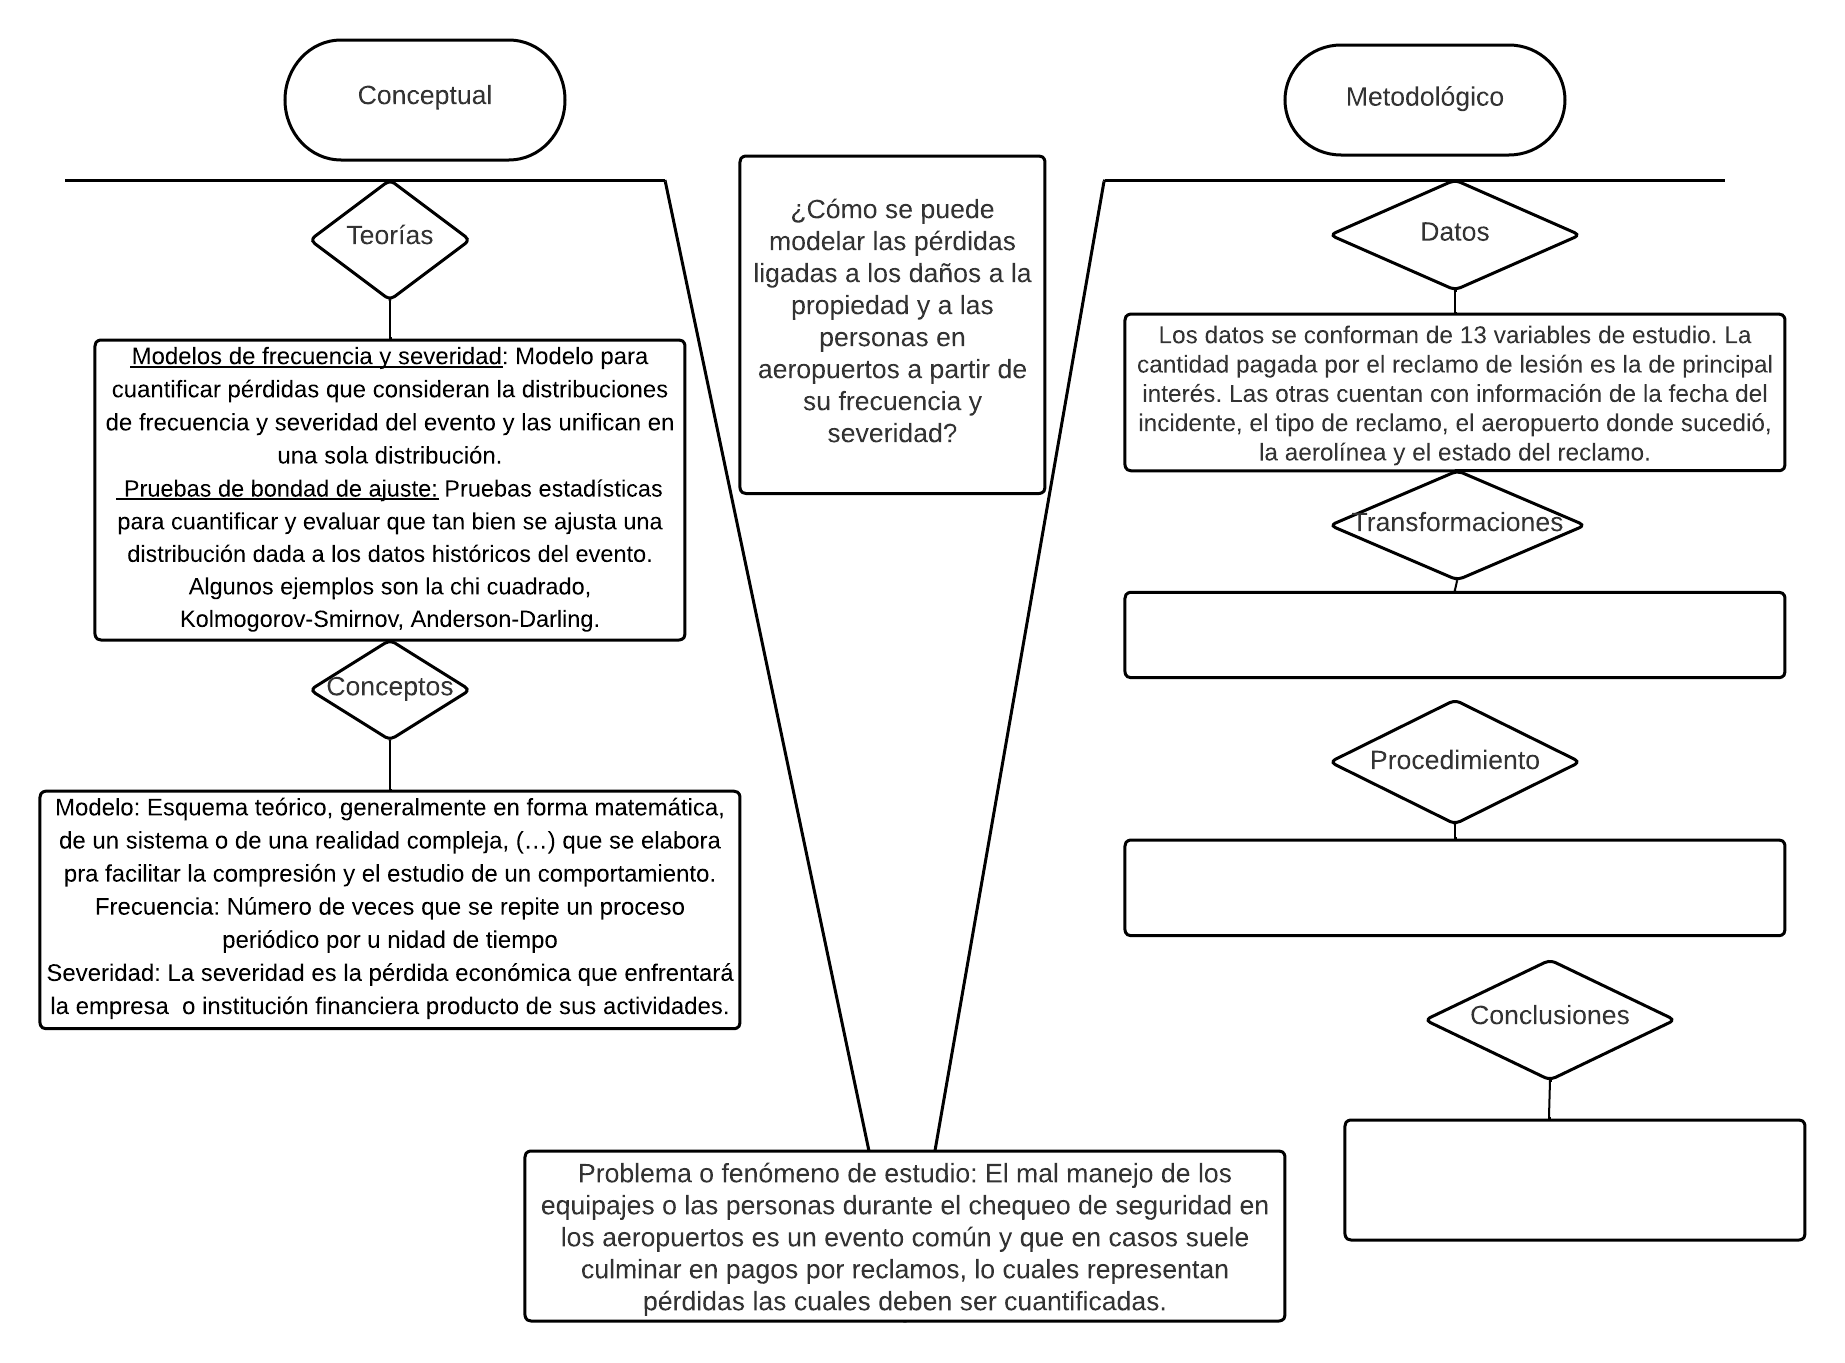
\includegraphics[width=6.25in,height=\textheight]{./Images/UVE Maik.png}

}

\end{figure}

\hypertarget{secciuxf3n-7.-descripciuxf3n-detallada-de-la-tabla-de-datos}{%
\subsubsection{Sección 7. Descripción detallada de la tabla de
datos}\label{secciuxf3n-7.-descripciuxf3n-detallada-de-la-tabla-de-datos}}

\textbf{Claim Number:} Es una variable de tipo \emph{string} que indica
el identificador del reclamo, cada vez que una persona procede a
efectuar un reclamo se le asigna este.

\textbf{Date Received:} Es una variable de tipo caracter, sin embargo
para efectos de estudio debe ser transformada a una variable tipo fecha.
El objetivo de esta variable es registrar el momento donde se realiza el
reclamo en el siguiente formato: día-mes-año.Hay un total de 263 NA , es
decir donde se registro reclamo respectivo pero no así la fecha. Esta
variable es importante para nuestro estudio,ya que se debe tomar en
cuenta el numero de reclamos al modelar las perdidas por frecuencia.

\textbf{Incident Date:} Se observa una diferencia de fechas desde el
momento que se lleva acabo el incidente y el momento de reclamo
correspondiente. Por esta razón se registra a fecha del incidente.

Esta es una variable de tipo caracter , la cual para efectos de estudio
debe ser transformada a una variable tipo fecha. Esta registra el
momento en que se lleva a cabo el incidente siguiendo el siguiente
formato: día/mes/año.Hay un total de 2183 NA , es decir , se llevo a
cabo el registro del reclamo pero no se tiene información de la fecha en
que se llevo a cabo el incidente.

Para efectos del modelado de la perdida por frecuencia la variable de
mayor interés para nuestro estudio es la ya mencionada \emph{Date
Received}.

\textbf{Airport Name:} Esta variable es una variable de tipo
\emph{string} categórica , hay un total de 466 Aeropuertos registrados
en la base de datos, un total de 8524 NA y 441 reclamos donde no se
especifica el nombre del Aeropuerto (se les establece el símbolo : -).

En esta se registra el nombre del aeropuerto donde se lleva acabo el
incidente.Esta variable aleatoria es importante , ya es posible saber
cuales son aquellos aeropuertos donde se presenta mayor número de
reclamos.

\textbf{Airport Code:} Los códigos de aeropuertos están formados por
grupos de tres letras, que designan a cada aeropuerto del mundo y
asignadas por la Asociación Internacional de Transporte Aéreo.

Esta variable es de tipo caracter, y registra dicho código del
aeropuerto donde se lleva a cabo el incidente por lo que aporta la misma
información que la variable aleatoria \emph{Airport Name} , para efectos
del estudio es importante considerar eliminar alguna de estas dos
variables.

\textbf{Airline Name:} Es una variable que registra la aerolínea en la
que viajaba la persona que sufrió el incidente. Es una variable tipo
\emph{string} categórica. Hay un total de 232 aerolíneas registradas en
la base de datos, un total de 34374 NA y 4247 reclamos donde no se
especifica el nombre de la aerolínea (se les establece el símbolo : -).

Esta variable es de interés para el desarrollo de nuestro estudio ya que
es importante saber cuales son las aerolíneas que presentan mayor número
de reclamos, y por ende si tienen una mayor impacto en las pérdidas.

\textbf{Claim type:} Esta variable es de tipo \emph{string} categórica,
la cual registra el tipo de reclamo realizado por la persona. Hay un
total 10 tipos de reclamos registrados en la base de datos:

\begin{itemize}
\item
  \emph{Bus Termina} : Categoría que registra reclamos relacionados a la
  terminal de buses, hay un 1 reclamo.
\item
  \emph{Complaint}: Categoría que registra reclamaciones de forma
  general, hay un total de 49 reclamos.
\item
  \emph{Compliment}: Categoría que registra quejas de forma general, hay
  un total de 3 reclamos.
\item
  \emph{Employee Loss (MPCECA)}: Categoría que registra reclamos por
  pérdidas de empleados (MPCECA).Es decir, reclamos de perdida
  realizados por los mismos empleados. Hay un total de 485.
\item
  \emph{Motor Vehicle}: Categoría que registra reclamos asociados
  vehiculos automotores , hay un total de 369 reclamos.
\item
  \emph{Passenger Property Loss} : Categoría que registra reclamos por
  pérdidas de bienes de los pasajeros. Esta es la categoría con mayor
  número de reclamos con un total de 117868 reclamos.
\item
  \emph{Passenger Theft}: Categoría que registra reclamos asociados
  robos realizados a bienes de los pasajeros , hay un total de 465
  reclamos.
\item
  \emph{Personal Injury} : Categoría que registra reclamos asociados a
  daños personales (siendo este un término legal para una lesión al
  cuerpo, la mente o las emociones, en contraposición a una lesión a la
  propiedad) hay un total de 1465 reclamos.
\item
  \emph{Property Damage}: Categoría que registra reclamos asociados
  daños a la propiedad. Esta es la segunda categoría con mayor cantidad
  de reclamos hay un total de 75364 reclamos.
\item
  \emph{Wrongful Death}: Categoría que registra reclamos asociados a
  muerte por negligencia , es un reclamo contra una persona que puede
  ser considerada responsable de la muerte de otra persona. Hay un total
  de 4 reclamos.
\end{itemize}

Finalmente, para esta variable hay un total de 7913 NA y 282 reclamos
donde no se especifica el tipo de reclamo (se les establece el símbolo :
-).

Esta variable es de interés , puesto que puede existir una relación
directa con el monto de los reclamos , y por ende tener impacto sobre la
perdida por severidad.

\textbf{Claim Site:} Esta variable es de tipo string categórica, la cual
indica el sitio del reclamo. Hay un total de 5 categorías registras para
esta variable: \emph{Bus Station} , \emph{Checked Baggage},
\emph{Checkpoint}, \emph{Motor Vehicle} y otra categoría llamada
\emph{others}.

Se observa que las categorías con mayor número de reclamos son:
\emph{Checked Baggage} con 159753 reclamos , y \emph{Checkpoint} con
40133 reclamos. Además, hay un total de 740 NA y 276 reclamos donde no
se especifica el nombre del Aeropuerto (se les establece el símbolo :
-).

\textbf{Item:} Esta variable es de tipo \emph{string} ,la cual se
encarga de describir el motivo de reclamo (bien material perdido, daño
material sufrido, daño personal).

\textbf{Claim Amount:} Esta variable es de tipo numérico,la cual se
encarga de registar el monto de reclamo.Es decir, el monto solicitado
por la persona que sufrió el incidente. Hay un total de 4043 NA y 12752
reclamos donde no se especifica el monto de reclamo (se les establece el
símbolo : -).

\textbf{Status:} Esta variable indica el estado intermedio del reclamo,
es de tipo \emph{string} categórica. Al no ser el status final del
reclamo cuenta con una cantidad considerable de categorías (14
registradas en la base de datos, 5 NA y 12752 reclamos donde no se
especifica el monto de reclamo donde se les establece el símbolo : -)
las cuales se terminan asignando en alguna de las tres categorías de la
variable \emph{Disposition} que a continuación se describe.

\textbf{Disposition:} Esta variable a diferencia de \emph{Status}
muestra la disposición , es decir el acuerdo final sobre el reclamo. Es
una variable de tipo string categórica , con tres categorías:
\emph{Approve in Full}, \emph{Deny} y \emph{Settle}. A continuación, se
describe cada una de estas:

\begin{itemize}
\item
  \emph{Approve in Full} : Esta categoría registra aquellos reclamos
  cuyo \emph{Claim Amount} (monto reclamado por la persona perjudicada)
  fue aprobado de forma total, es decir, el monto acordado a pagar
  (\emph{Close Amount}) es igual al \emph{Claim Amount}. Hay un total de
  35010 reclamos aprobados de forma completa.
\item
  \emph{Deny}: Esta categoría registra los reclamos denegados, es decir
  aquellos reclamos donde no se paga por el reclamo. Hay un total de
  68382 reclamos denegados.
\item
  \emph{Settle}: En esta categoría se registran aquellos reclamos cuyo
  \emph{Close Amount} (monto a pagar) , es menor al \emph{Claim Amount}
  (Monto de reclamo). Es decir, son aquellos reclamos en cuyo acuerdo
  final se estableció un monto inferior de pago por el incidente.
\end{itemize}

\textbf{Close Amount:} Esta variable es de tipo numérica, y es el monto
final acordado por ambas partes.Es decir, es el monto que debe ser
pagado a la persona como producto del reclamo realizado. Es importante
señalar que este monto es igual o inferior al \emph{Claim Amount} y
depende de la variable disposición que se describió anteriormente. Esta
variable es relevante para nuestro estudio pues esta relacionado de
forma directa con la severidad, y por ende, con la perdida por
severidad.

\hypertarget{secciuxf3n-8.-literatura}{%
\subsubsection{Sección 8. Literatura}\label{secciuxf3n-8.-literatura}}

\begin{enumerate}
\def\labelenumi{\arabic{enumi}.}
\item
  \textbf{Título}: Modelling Dependencies in Airport Passenger Claim
  Data Using Copulas (Flores, 2022) \textbf{Autor:} Roberto Carcache
  Flores

  \textbf{Nombre del tema}: Modelación del riesgo utilizando cópulas

  \textbf{Forma de organizarlo}:

  \begin{itemize}
  \item
    Cronológico: Febrero 2022
  \item
    Metodológico: Cópulas bivariadas y multivariadas y simulaciones
  \item
    Temático: Funciones de distribución y dependencia de variables
    aleatorias
  \item
    Teoría: Probabilidad y estadística
  \end{itemize}

  \textbf{Resumen en una oración}: Se encuentra la mejor distribución
  para la severidad y frecuencia de cada reclamo y luego estas
  distribuciones marginales se incorporan en diferentes modelos de
  cópulas

  \textbf{Argumento central}: En la metodología tradicional del
  modelamiento del riesgo se asume independencia entre frecuencia y
  severidad, lo cual no se hace en esta investigación. Además, se
  utiliza un proceso de eliminación de la tendencia con respecto al
  tiempo para mejorar los resultados.

  \textbf{Problemas con el argumento o el tema:} Las medidas de riesgo
  utilizando cópulas resultan en medidas de riesgo más altas que en los
  datos históricos.

  \textbf{Resumen en un párrafo}: Se eliminan los reclamos que fueron
  negados justificando el hecho de que el punto de la investigación es
  cuantificar los pagos que efectivamente fueron hechos, además del gran
  volumen de los datos. La agregación de los datos se hace por mes y con
  suma para la severidad y por frecuencia de los reclamos. El autor nota
  que hay un tendencia negativa de la frecuencia y severidad con
  respecto al tiempo por lo que procede a eliminar la tendencia. Luego
  determina la mejor marginal para cada variable utilizando MLE. Se
  encuentra que la binomial negativa se ajusta mejor a las frecuencias.
  Por otro lado la Log-Laplace se ajusta mejor a los reclamos por daños
  a la propiedad y la lognormal se ajusta mejor a los reclamos por
  pérdidas de los bienes por lo que se utilizan estas dos para modelar
  la severidad. Luego se procede a hacer algo similar con los resultados
  de eliminar la tendencia. Se encuentra que el proceso de eliminación
  de la tendencia facilita la búsqueda de una distribuciones. Se
  encuentra que todas las variables pares muestran algún tipo de
  dependencia en las colas. Finalmente, las cópulas multivariadas se
  comparan utilizando log verosimilitud y se obtiene que las cópulas
  elípticas (Gaussiana y t-Student) se ajustan mejor que las
  arquimedianas (Clayton y Gumbel).
\item
  \textbf{Título}: Aggregate loss model with Poisson - Tweedie loss
  frequency (Chen, 2020)

  \textbf{Autor:} Si Chen.

  \textbf{Nombre del tema}: Modelado perdidas usando la familia de
  distribuciones Poisson - Tweedie .

  \textbf{Forma de organizarlo}:

  \begin{itemize}
  \item
    Cronológico: Año 2020.
  \item
    Metodológico: Modelado de la frecuencia de perdida a partir de una
    distribución Poisson-Tweedie , simulaciones y modelado de perdida
    agregada.
  \item
    Temático: Modelos de perdida agregada.
  \item
    Teoría: Distribuciones de perdidas.
  \end{itemize}

  \textbf{Resumen en una oración}: Uso de la familia de distribuciones
  Poisson-Tweedie con la finalidad de modelar la frecuencia de las
  perdidas y ver el impacto que tiene este sobre el modelo de perdidas
  agregadas.

  \textbf{Argumento central}: Pese a que el impacto de la perdida por
  severidad en un modelo de perdida agregada ha sido bien estudiado a
  través de los años, se ha prestado menos atención a la influencia de
  la perdida por frecuencia en dichos modelos, esto motiva el estudio de
  un modelo de perdidas por frecuencias no tradicional.

  \textbf{Problemas con el argumento o el tema:} Dado el estudio , no se
  pudo captar por completo las relaciones entre las perdidas por
  severidad , perdida por frecuencia y perdida agregada.

  \textbf{Resumen en un párrafo}: En este estudio, se modela la perdida
  por frecuencia usando la familia de distribuciones Poisson-Tweedie,
  esto bajo el argumento que dichas familias presentan características
  como: el ajuste de la frecuencia de pérdidas es más flexible , reducen
  la posibilidad de una especificación errónea del modelo y dichas
  familias presentan una convolución cerrada. Mediante estudios de
  simulación , se investiga y encuentra el impacto de una mala
  especificación de la distribución perdida de la frecuencia al cuantil
  de perdidas agregadas, así como el sesgo del estimador de máxima
  verosimilitud del índice de la familia de Poisson-Tweedie.
\item
  \textbf{Título}: \emph{Estimation of Parametric and Nonparametric
  Models for Univariate Claim Severity Distributions - an approach using
  R} (Pitt et~al., 2011)

  \textbf{Autores:} David Pitt, Montserrat Guillen y Catalina Bolancé

  \textbf{Nombre del tema}: Comparación de métodos paramétricos y no
  paramétricos apra modelar la severidad de reclamos en una aseguradora

  \textbf{Forma de organizarlo}:

  \begin{itemize}
  \item
    Cronológico: mayo de 2011
  \item
    Metodológico: estimación de densidades por Kernels modificados,
  \item
    Temático: Modelación de reclamos métidos y de seguros de automóviles
  \item
    Teoría: Probabilidad y estadística
  \end{itemize}

  \textbf{Resumen en una oración}: Se encuentra que la estimación por
  kernels modificados es adecuada para modelar la distribución tanto de
  costos médicos como de reclamos en seguros de automóviles.

  \textbf{Argumento central}: Se pueden usar métodos no paramétricos
  para estimar distribuciones de reclamos en seguros de vehículo y de
  costos médicos.

  \textbf{Problemas con el argumento o el tema:} Los métodos clásicos de
  estimación de densidades por kernels suelen ser inadecaudos en
  presencia de asimetría, lo cual es común en datos de montos de
  reclamos en el contexto de seguros.

  \textbf{Resumen en un párrafo}: Se utilizan datos de costos de
  reclamos hechos a una aseguradora española por accidentes ocurridos en
  el año 2000 y recopilados en 2002, que incluye tanto los ligados a
  costos por daños a la propiedad como por costos médicos. El tamaño de
  muestra es de 518 reclamos. Para estimar la densidad para cada uno de
  los costos (daños a la propiedad y médicos) por separado, se utilizan
  métodos paramétricos y no paramétricos. Dentro de los paramétricos, se
  utilizaron aproximaciones normales y log-normales. Dentro de los no
  paramétricos, se utilizó una aproximación por kernels modificada,
  donde la modificación consiste en que primero se aplica una
  transformación a los datos originales para corregir la asimetría, se
  hace una aproximación con un kernel gaussiano a los datos modificados,
  y luego se calcula la aproximación de los datos originales a partir de
  la calculada para los modificados. La transformación aplicada a los
  datos se enmarca en la \emph{shifted power transformation family}.
  Para evaluar la bondad de ajuste de todas las estimaciones propuestas,
  se utilizan distintas versiones log-verosimilitud tanto la versión
  clásica como modificaciones ponderadas, mientras que para evaluar
  solamente los métodos no paramétricos se usan distintas versiones de
  una aproximación a errores cuadráticos integrados ponderados. Se
  concluye que la log-verosimilitud no es una buena medida de bondad de
  ajuste para comparar los ajustes no paramétricos, debido a su relación
  inversa con la magnitud del ancho de banda empleado. En general, de
  las propuestas paramétricas, la log-normal tuvo un mejor desempeño
  mientras que la estimación por kernel modificada tuvo un desempeño
  adecuado y se recomienda para modelar distribuciones con colas
  pesadas.
\item
  \textbf{Título}: \emph{Estimation of Parametric and Nonparametric
  Models for Univariate Claim Severity Distributions - an approach using
  R} (Ondieki et~al., 2018)

  \textbf{Autores:} Cyprian Ondieki, Shalyne Gathoni y Joan Wairimu

  \textbf{Nombre del tema}: Estimación de distribuciones de frecuencia y
  severidad en seguros de automóviles

  \textbf{Forma de organizarlo}:

  \begin{itemize}
  \item
    Cronológico: febrero de 2018
  \item
    Metodológico: Distribuciones continuas para la modelización de la
    severidad y discretas para la modelización de la frecuencia, donde
    los parámetros se estiman por máxima verosimilitud y los ajustes se
    miden con pruebas chi cuadrad, Kolmogorov-Smirnov, Anderson-Darling
    y los modelos se seleccionan de acuerdo a sus medidas de AIC y BIC.
  \item
    Temático: Modelización de la frecuencia y severidad en seguros de
    automóviles
  \item
    Teoría: Probabilidad y estadística, distribuciones probabilísticas,
    pruebas de bondad de ajuste, estimación por máxima verosimilitud
  \end{itemize}

  \textbf{Resumen en una oración}: Se ponen a prueba varias
  distribuciones para estimar la distribución tanto de frecuencia como
  la severidad de reclamos de automóviles de tres bases de datos
  distintas.

  \textbf{Argumento central}: En el contexto de seguros de automóviles,
  la distribución lognormal es apropiada para modelizar la severidad y
  la binomial negativa y geométrica lo son para modelizar la frecuencia.

  \textbf{Problemas con el argumento o el tema:} Se advierte que
  pronósticos realizados con los modelos seleccionados pueden ser
  C:tiles solamente en el corto plazo. Además, no se consideran
  distribuciones de la clase \((a,b,1)\).

  \textbf{Resumen en un párrafo}: Con tres bases de seguros de
  automóviles gratuitas en R (\emph{AutoCollision}, \emph{dataCar},
  \emph{dataOhlsson}) se proponen distribuciones continuas para la
  modelización de la severidad (Exponencial, Gamma, Pareto, Lognormal y
  Weibull) y discretas para la modelización de la frecuencia (Binomial,
  Geométrica, Binomial Negativa, Poisson), donde los parámetros se
  estiman por máxima verosimilitud y los ajustes se miden con pruebas
  chi cuadrado (para la frecuencia) y Kolmogorov-Smirnov y
  Anderson-Darling (para la severidad), así como se usa el Criterio de
  Información de Akaike (AIC) y el Criterio de Información Bayesiano
  (BIC) para determinar el mejor modelo de los no descartados con las
  pruebas anteriores. Se concluye que la distribución que constituye el
  mejor modelo para la severidad es la lognormal, mientras que en cuanto
  a la frecuencia, las más adecuadas son la binomial negativa y la
  geométrica.
\end{enumerate}

\hypertarget{teoruxedas-principios-o-metodologuxedas}{%
\subsection{Teorías, principios o
metodologías}\label{teoruxedas-principios-o-metodologuxedas}}

\textbf{Elección de los modelos de frecuencia y severidad:}

Con la finalidad de modelar la frecuencia con la que ocurren los
reclamos por extravío y la severidad de estos, se desea contar con los
modelos que mejor se ajusten a nuestro estudio en cuestión.

No obstante, existe una serie de distribuciones de probabilidad estándar
que se podrían utilizar para aproximar las distribuciones de las
variables aleatorias de la frecuencia de reclamaciones y la severidad o
monto de estas reclamos. Las distribuciones binomial, geométrica,
binomial negativa y Poisson se consideran para la modelización de la
frecuencia.

Por otro lado, entre las distribuciones estándar para modelar la
severidad se tienen las siguientes distribuciones: exponencial, gamma,
Weibull, Pareto y lognormal.

Tal como lo establece Ondieki et~al. (2018) una forma de abordar la
escogencia de la distribución correcta es ajustando los datos a las
distribuciones estadísticas seleccionadas y los parámetros se estiman
mediante el método de máxima verosimilitud.

Una vez ajustas las distribuciones a los datos y estimados los
parámetros es posible hacer pruebas de bondad de ajuste para ambos
modelos, y pruebas para elegir entre las distribuciones que compiten
entre sí. A continuación se establecen cuales son estas pruebas.

\textbf{Elección de los modelos de frecuencia y severidad:}

Una prueba de bondad de ajuste es ``un procedimiento estadístico que
describe qué tan bien se ajusta una distribución a un conjunto de
observaciones mediante la medición de la compatibilidad cuantificable
entre las distribuciones teóricas estimadas y la distribución empírica
de los datos muestrales'' (Ondieki et~al., 2018). Estas pruebas se
pueden basar en la función de densidad o masa o en la función de
distribución y adoptan la estructura de prueba de hipótesis donde la
hipótesis nula consiste en que los datos siguen una distribución
particular, mientras que la alternativa en que los datos no siguen dicha
distribución particular.

Se presenta ahora una idea general de las tres pruebas de bondad de
ajuste que se proponen para este análisis:

\begin{itemize}
\item
  Prueba Chi-Cuadrado de bondad de ajuste: Esta prueba propone un
  estadístico compuesto de frecuencias observadas y esperadas, calculado
  a partir de una partición de la muestra, el cual presenta bajo la
  hipóstesis nula una distribución Chi-Cuadrado con grados de libertad
  que dependen de la cantidad de datos, la cantidad de intervalos de la
  partición y la cantidad de parámetros de la distribución propuesta
  calculados por medio de los datos muestrales.
\item
  Prueba Kolmogorov-Smirnov: Esta prueba se basa en comparar la función
  de distribución propuesta con la función de distribución empírica de
  los datos para medir el ajuste, partiendo de que la función de
  distribución caracteriza a una distribución de probabilidad. Esta
  comparación se realiza mediante un estadístico que mide la distancia
  entre ambas distribuciones, del cual se conocen ciertos resultados de
  convergencia y distribución que fundamentan la efectividad del método.
\item
  Prueba Anderson-Darling: Esta prueba se asemeja a la de
  Kolmogorov-Smirnov pero mide de una forma distinta la diferencia en
  tre las funciones de distribución empírica y teórica. Además, de
  acuerdo a Klugman et~al. (2019) el estadístico de prueba de
  Anderson-Darling suele priorizar un mejor ajuste en las colas de la
  distribución en comparación con las regiones más centrales.
\end{itemize}

En las bitácoras posteriores se ampliará en los aspectos técnicos de las
pruebas anteriormente mencionadas.

\hypertarget{parte-de-escritura}{%
\section{Parte de escritura}\label{parte-de-escritura}}

\hypertarget{secciuxf3n-1.-escogencia-de-la-pregunta-de-investigaciuxf3n}{%
\subsection{Sección 1. Escogencia de la pregunta de
investigación}\label{secciuxf3n-1.-escogencia-de-la-pregunta-de-investigaciuxf3n}}

La pregunta seleccionada es la primera: \emph{¿Cómo se puede modelar las
pérdidas ligadas a los daños a la propiedad y a las personas en
aeropuertos a partir de su frecuencia y severidad?}

Se cambió ``extravío de equipajes'' por ``daños a la propiedad y a las
personas'' para poder abarcar el resto de eventos que aparecen en la
base de datos.

\hypertarget{secciuxf3n-2.-propuesta-de-argumentaciuxf3n}{%
\subsection{Sección 2. Propuesta de
argumentación}\label{secciuxf3n-2.-propuesta-de-argumentaciuxf3n}}

En general, el modelado de las pérdidas es de vital importancia ya que
permite a las empresas, entidades financieras y aseguradoras tener
reservas para lograr mitigar el impacto de dichas pérdidas. Tal y como
establece Ondieki et~al. (2018), para las aseguradoras poder liquidar
los siniestros que puedan llegar a producirse esto es fundamental, por
lo que es imperativo que se modelice adecuadamente los datos históricos
y actuales sobre la experiencia de los siniestros, permitiendo de esta
forma proyectar las experiencia de los siniestros futuros esperados y
establecer reservas suficientes.

Una forma de realizar este ejercicio de modelación es utilizando una
base proveniente del Departamento de Seguridad Nacional de Estados
Unidos, quienes manejan la seguridad en más de 400 aeropuertos de dicho
país a través de TSA (Transportation Security Administration). En la
revisión de la literatura se ubican dos fuentes que emplean esta base de
datos y que persiguen objetivos similares, que son los trabajos de
Flores (2022) y Chen (2020). De esta manera, se comprueba que la fuente
de la base de datos ha sido validada antes en investigaciones de corte
académico y estrechamente relacionadas con el tema del presente escrito,
además de estar adecuadamente referenciada y poder consultarse en Kelly
\& Wang (2020).

Para contestar la pregunta de investigación, se propone seguir el
procedimiento adoptado en Ondieki et~al. (2018), en el se parte de un
grupo de distribuciones continuas para la modelización de la severidad
(Exponencial, Gamma, Pareto, Lognormal y Weibull) y otro de
distribuciones discretas para la modelización de la frecuencia
(Binomial, Geométrica, Binomial Negativa, Poisson), donde los parámetros
se estiman por máxima verosimilitud y los ajustes se miden con pruebas
Chi-Cuadrado (para la frecuencia) y Kolmogorov-Smirnov y
Anderson-Darling (para la severidad). También, en dicha investigación se
usa el Criterio de Información de Akaike (AIC) y el Criterio de
Información Bayesiano (BIC) para determinar el mejor modelo de los no
descartados con las pruebas anteriores. Adicionalmente, se contempla
incorporar distribuciones truncadas y modificadas en búsqueda de ajustes
superiores.

\hypertarget{secciuxf3n-3.-resumen-del-problema-hasta-el-momento.}{%
\subsection{Sección 3. Resumen del problema hasta el
momento.}\label{secciuxf3n-3.-resumen-del-problema-hasta-el-momento.}}

El TSA (Transportation Security Administration) es la agencia
establecida luego del 2001 que se ocupa del chequeo de los pasajeros y
su equipaje en los aeropuertos de Estados Unidos. Como consecuencia de
sus labores, es común que se causen daños y extravíos de las
pertenencias de los pasajeros lo que resulta en reclamos por parte de
los mismos en la forma de compensación monetario por los daños
ocassionados. Estos pagos han sido registrados en la tabla que se
utilizará para esta investigación, además de otra información pertinente
a cada incidente reclamado. El propósito de este trabajo será el de
modelar estas pérdidas para lograr cuantificarlas. Esto es importante
pues el TSA tiene que tener previsto estos costos para poder continuar
sus operaciones, y los pasajeros que sí son víctimas del mal manejo de
sus pertenencias puedan conseguir su dinero devuelta.

Al consultar la literatura se ha visto que este es un problema que ha
sido tratado por al menos dos trabajos anteriores en los cuales se
basará esta investigación con el fin de expandir y poder comparar y
contrastar los resultados que se obtienen con los de ellos. En general
se han identificados varios pasos que se deberán seguir para poder
lograr el cometido. Primero se busca la densidad apropiada para la
frecuencia y severidad por separado mediante la estimación del parámetro
MLE. Las densidades candidatas para la frecuencia son la binomial
negativa, geométrica, Poisson y binomial. Por otro lado, las candidatas
para la densidad de la severidad son la log-normal, log-laplace, Johnson
SU y la logística generalizada. Sin embargo, a través del trabajo se
investigará otras posibles distribuciones que pueden ser de utilidad. La
bondad de ajuste para comparar las distribuciones anteriores se lleva a
cabo utilizando pruebas como la chi cuadrado, Kolmogorov-Smirnov y
Anderson Darling.

Una vez obtenidas las distribuciones se deben unificar en un modelo
agregada que represente las pérdidas totales utilizando cópulas
bivariadas o multivariadas. Algunos ejemplos de las que sea han
utilizado son la Clayton y la Gumbel. Estas son comparadas mediante la
utilización de medida empírica UTDC para escoger la más apropiada para
el problema en cuestión. Otra observación importante es que algunos
autores noten que existe una tendencia de las pérdidas con respecto al
tiempo por lo que el primer paso en realidad es la eliminación de dicha
tendencia. Este paso puede ser importante pues notan que al comparar el
proceso descrito anteriormente al haber eliminado la tendencia se
lograban mejores resultados. Sin embargo, esta es otra capa de
complejidad que será evaluada durante el proceso si se incluye o no.

Algunos otros hallazgos importantes aparte del impacto positivo que
tiene la elimnación de la tendencia, es que encontró que la binomial
negativa se ajusta mejor a las frecuencias, mientras que la Log-Laplace
se ajusta mejor a la severidad de los daños a la propiedad, y la
Log-lognormal a los extravíos. Luego para las cópulas se encuentra que
cópulas elípticas (Gaussiana y t-Student) se ajustan mejor que las
arquimedianas (Clayton y Gumbel).

\bookmarksetup{startatroot}

\hypertarget{bituxe1cora-2}{%
\chapter{Bitácora 2}\label{bituxe1cora-2}}

Para esta bitácora se decidió mudar el análisis a otra base de datos
(también de reclamos a TSA), pues al revisar con más detalle la
anterior, que comprendía datos del periodo 2002-2015, como parte del
análisis descriptivo se notó que los datos de la variable más importante
para este trabajo, que es \emph{close\_amount} (monto final pagado por
cada reclamo), no estaba presente del todo a partir del año 2010. Esto
marca una inconsistencia ya que al revisar los archivos de TSA para el
periodo 2010-2013 se comprobó que los datos para la mencionada variable
sí estaban disponibles. Por esta razón, se decidió trabajar con esta
segunda base de datos, es decir la que contempla solamente de 2010 a
2013 y en lo sucesivo los análisis se refieren a este periodo de menor
duración.

\hypertarget{ordenamiento-de-la-literatura}{%
\section{Ordenamiento de la
literatura}\label{ordenamiento-de-la-literatura}}

\hypertarget{tbl-ordenamiento}{}
\begin{table}
\caption{\label{tbl-ordenamiento}Ordenamiento de la literatura }\tabularnewline

\centering
\begin{tabu} to \linewidth {>{\raggedright}X>{\raggedright}X>{\raggedright}X>{\raggedright}X>{\raggedleft}X>{\raggedright}X}
\hline
\textbf{Tipo de grupo} & \textbf{Nombre del grupo} & \textbf{Nombre del tema} & \textbf{Título} & \textbf{Año} & \textbf{Autor (es)}\\
\hline
Metodológico & Modelo de cópulas & Modelación de distribuciones de pérdidas & Modelling Dependencies in Airport Passenger Claim Data Using Copulas & 2022 & Roberto Carcache Flores\\
\hline
Metodológico & Modelos de pérdidas agregadas & Modelación paramétrica de distribuciones de pérdidas & Aggregate loss model with Poisson - Tweedie loss frequency & 2020 & Si Chen\\
\hline
Metodológico & Estimación de densidades por kernels & Modelación no paramétrica de distribuciones de pérdidas & Estimation of Parametric and Nonparametric Models for Univariate Claim & 2011 & David Pitt, Montserrat Guillen y Catalina Bolancé\\
\hline
Metodológico & Modelos de frecuencia y severidad & Modelación de las distribuciones de frecuencia y severidad & Severity Distributions - an approach using R & 2018 & Cyprian Ondieki, Shalyne Gathoni y Joan Wairimu\\
\hline
\end{tabu}
\end{table}

\newpage

\hypertarget{enlaces-de-la-literatura}{%
\section{Enlaces de la literatura}\label{enlaces-de-la-literatura}}

En Flores (2022) se establece el procedimiento base para conseguir la
distribución agregada al igual que algunos hallazgos y metodologías que
son de alta utilidad. Primero la agregación de los datos se hace
mensualmente con suma para la severidad y por frecuencia para los
reclamos. El autor nota que hay un tendencia negativa de la frecuencia y
severidad con respecto al tiempo por lo que procede a eliminarla. Luego,
determina la mejor distribución para cada variable utilizando estimación
de máxima verosimilitud (MLE). Se encuentra que la binomial negativa se
ajusta mejor a las frecuencias. Por otro lado, la Log-Laplace se ajusta
mejor a los reclamos por daños a la propiedad y la lognormal se ajusta
mejor a los reclamos por pérdidas de los bienes, por lo que se utilizan
estas dos para modelar la severidad. Durante este proceso el autor nota
que la eliminación de la tendencia facilita el proceso de ajustar una
distribución a la frecuencia y la severidad. Finalmente, las cópulas
multivariadas se comparan utilizando log\_añoverosimilitud y se obtiene
que las cópulas elípticas (Gaussiana y t-Student) se ajustan mejor que
las arquimedianas (Clayton y Gumbel).

En un estudio similar, Pitt et~al. (2011) utilizan datos de costos de
reclamos hechos a una aseguradora española por accidentes ocurridos en
el año 2000 y recopilados en 2002, que incluye tanto los ligados a
costos por daños a la propiedad como por costos médicos. El tamaño de
muestra es de 518 reclamos. Al igual que el estudio anterior, para
estimar la densidad para cada uno de los costos (daños a la propiedad y
médicos) se utilizan métodos paramétricos como las aproximaciones
normales y log-normales. En contraste al estudio pasado también recurren
a estimadores no paramétricos como la aproximación por kernels
modificada, donde la modificación consiste en que primero se aplica una
transformación a los datos originales para corregir la asimetría, se
hace una aproximación con un kernel gaussiano a los datos modificados, y
luego se calcula la aproximación de los datos originales a partir de la
calculada para los modificados. La transformación aplicada a los datos
se enmarca en la \emph{shifted power transformation family}.

Adicionalmente, los mismos autores exponen métodos para evaluar la
bondad de ajuste de las distribuciones encontradas. Para evaluar todas
las estimaciones propuestas se utiliza la log-verosimilitud, tanto la
versión clásica como modificaciones ponderadas, mientras que para
evaluar solamente los métodos no paramétricos se usan distintas
versiones de una aproximación a errores cuadráticos integrados
ponderados. Se concluye que la log-verosimilitud no es una buena medida
de bondad de ajuste para comparar los ajustes no paramétricos, debido a
su relación inversa con la magnitud del ancho de banda empleado. En
general, de las propuestas paramétricas, la log-normal tuvo un mejor
desempeño, el cual es un hallazgo que concuerda con el de Flores (2022),
mientras que la estimación por kernel modificada tuvo un desempeño
adecuado y se recomienda para modelar distribuciones con colas pesadas.

El modelado de pérdidas agregadas es una técnica estadística ampliamente
utilizada en el ámbito actuarial, cuyo objetivo es la obtención de una
función de distribución de perdidas agregadas, a partir de la
distribución de frecuencia de reclamos, y de la distribución de la
severidad de estos.

Un claro ejemplo de la implementación de esta técnica es el estudio
realizado por (Chen, 2020) . La principal motivación de este estudio es
la de modelar la frecuencia de las pérdidas mediante el uso de la
familia de distribuciones Poisson-Tweedie con la finalidad de modelar la
frecuencia de las perdidas y ver el impacto que tiene este sobre el
modelo de pérdidas agregadas.

Esto bajo el argumento que dichas familias presentan características
como: el ajuste de la frecuencia de pérdidas es más flexible , reducen
la posibilidad de una especificación errónea del modelo y dichas
familias presentan una convolución cerrada.

Mediante el uso de la distribución de la familia Poisson-Tweedie y el
estudio de simulación basados en: Percentil de la distribución de
pérdidas agregadas bajo diferentes distribuciones de frecuencia de
pérdidas (diferentes valores del parámetros de la familia ) y la
investigación de estimadores de parámetros para frecuencia de pérdidas
vía simulaciones de Monte Carlo, se investiga y encuentra el impacto de
una mala especificación de la distribución perdida de la frecuencia al
cuantil de pérdida agregadas, así como el sesgo del estimador de máxima
verosimilitud del índice de la familia de Poisson-Tweedie.

Una de las principales diferencias de los métodos implementados en el
estudio realizado por (Chen, 2020) es el uso de máxima verosimilitud y
la implementación de simulaciones vía Monte Carlo. A diferencia de los
métodos empleados por (Pitt et~al., 2011) donde su estudio se centra en
la comparación entre métodos paramétricos tradicionales, y métodos no
paramétricos basados en la estimación de densidades por Kernels
modificados.

No obstante, pese a que según (Pitt et~al., 2011) se logra estimar de
forma adecuada la distribución tanto de costos médicos como de reclamos
en seguros de automóviles, los métodos clásicos de estimación de
densidades por kernels suelen ser inadecuados en presencia de asimetría,
siendo esto habitual en datos de montos de reclamos.

Pese a que el método de estimación de densidades por kernels es
técnicamente más sencillo que la implementación de los métodos
utilizados por (Chen, 2020) , es importante tomar en consideración los
problemas presentes en el estudio realizados por (Pitt et~al., 2011) ,
ya que pueden generar dificultades técnicas importantes.

Además, el uso de máxima verosimitud por parte de (Chen, 2020) para la
escogencia de los parámetros es un método de uso más frecuente, para
resolver problemas de esta índole.

Sin embargo, debido al enfoque de hace uso de una familia particular
para modelar la frecuencia.No obstante, es importante señalar que
existen test y pruebas especificas para escoger las distribuciones más
adecuadas dada la base de datos de un estudio en particular. Estas
técnicas estadísticas para la escogencia de las mejores distribuciones
tanto de a frecuencia como la severidad son empleadas por (Ondieki
et~al., 2018) .

(Ondieki et~al., 2018) hace uso de tres bases de seguros de automóviles
gratuitas en R (AutoCollision, dataCar, dataOhlsson), en su estudio
propone el modelado de la severidad mediante distribuciones continuas
(Exponencial, Gamma, Pareto, Lognormal y Weibull) y discretas (Binomial,
Geométrica, Binomial Negativa, Poisson) para el caso de la frecuencia,
donde los parámetros se estiman vía máxima verosimilitud y los ajustes
se miden con pruebas chi cuadrado (para la frecuencia) ,
Kolmogorov-Smirnov y Anderson-Darling\_año(para la severidad).

Una vez obtenidos los parámetros y realizadas las pruebas de ajuste, se
seleccionan los modelos de acuerdo a sus medidas del Criterio de
Información de Akaike (AIC) AIC y el Criterio de Información Bayesiano
(BIC).

Se concluye que la distribución que constituye el mejor modelo para la
severidad es la lognormal, mientras que en cuanto a la frecuencia, las
más adecuadas son la binomial negativa y la geométrica.

A diferencia del estudio realizado por (Ondieki et~al., 2018) en el cual
usa conjuntamente métodos paramétricos y no paramétricos con el objetivo
de compara estos, en este caso (Ondieki et~al., 2018) se enfoca en
utilizar un método paramétrico ampliamente utilizado como lo es la
estimación de parámetros vía máxima verosimilitud.Sin embargo, se enfoca
en implementar una gran variedad de pruebas, test y métricas para
obtener las mejores distribuciones posibles tanto de la frecuencia como
la severidad.

Es importante señalar que en el estudio de (Ondieki et~al., 2018) no se
realiza ninguna técnica para encontrar una distribución de perdidas
agregadas, a diferencia del estudio de (Chen, 2020) donde si construyen
esta distribución agregada.

Pese a que las técnicas estadísticas implementadas por Ondieki et~al.
(2018) son las tradicionales, a diferencia de los otros estudios
mencionados en este apartado, sí se tiene como objetivo escoger las
mejores distribuciones para la frecuencia y severidad para nuestro
estudio, es prudente seguir una línea de investigación similar a las
empleadas en este estudio. El implementar métodos no paramétricos como
el de densidades por kernels puede traer complejidades técnicas. Además,
el uso de una sola familia en particular como la Poisson-Tweedie tal y
como lo expuesto por (Chen, 2020) puede limitar la escogencia del mejor
modelo que describa de forma apropiada nuestra pregunta de
investigación.

\hypertarget{anuxe1lisis-estaduxedstico}{%
\section{Análisis Estadístico}\label{anuxe1lisis-estaduxedstico}}

\hypertarget{tbl-headDatos}{}
\begin{table}
\caption{\label{tbl-headDatos}Primeras cinco filas de la tabla de datos }\tabularnewline

\centering
\resizebox{\linewidth}{!}{
\begin{tabular}[t]{>{\raggedleft\arraybackslash}p{3cm}>{\raggedleft\arraybackslash}p{3cm}>{\raggedleft\arraybackslash}p{3cm}>{\raggedleft\arraybackslash}p{3cm}>{\raggedleft\arraybackslash}p{3cm}>{\raggedleft\arraybackslash}p{3cm}>{\raggedleft\arraybackslash}p{3cm}>{\raggedleft\arraybackslash}p{3cm}>{\raggedleft\arraybackslash}p{3cm}>{\raggedleft\arraybackslash}p{3cm}>{\raggedleft\arraybackslash}p{3cm}}
\toprule
\textbf{claim\_number} & \textbf{date\_received} & \textbf{incident\_date} & \textbf{airport\_code} & \textbf{airport\_name} & \textbf{airline\_name} & \textbf{claim\_type} & \textbf{claim\_site} & \textbf{item\_category} & \textbf{close\_amount} & \textbf{disposition}\\
\midrule
\cellcolor{gray!6}{2.010011e+12} & \cellcolor{gray!6}{2010-01-04} & \cellcolor{gray!6}{2010-01-03 14:30:00} & \cellcolor{gray!6}{SLC} & \cellcolor{gray!6}{Salt Lake City International Airport} & \cellcolor{gray!6}{Delta Air Lines} & \cellcolor{gray!6}{Property Damage} & \cellcolor{gray!6}{Checked Baggage} & \cellcolor{gray!6}{Cosmetics \& Grooming} & \cellcolor{gray!6}{0} & \cellcolor{gray!6}{Deny}\\
2.010011e+12 & 2010-01-04 & 2010-01-02 00:00:00 & LAX & Los Angeles International Airport & Southwest Airlines & Passenger Property Loss & Checked Baggage & Other & 0 & Deny\\
\cellcolor{gray!6}{2.010011e+12} & \cellcolor{gray!6}{2010-01-04} & \cellcolor{gray!6}{2010-01-02 05:00:00} & \cellcolor{gray!6}{SEA} & \cellcolor{gray!6}{Seattle-Tacoma International} & \cellcolor{gray!6}{Delta Air Lines} & \cellcolor{gray!6}{Passenger Property Loss} & \cellcolor{gray!6}{Checked Baggage} & \cellcolor{gray!6}{Cameras; Cameras} & \cellcolor{gray!6}{0} & \cellcolor{gray!6}{Deny}\\
2.010011e+12 & 2010-01-04 & 2010-01-01 00:00:00 & DEN & Denver International Airport & Southwest Airlines & Passenger Property Loss & Checked Baggage & Clothing & NA & -\\
\cellcolor{gray!6}{2.010011e+12} & \cellcolor{gray!6}{2010-01-04} & \cellcolor{gray!6}{2010-01-02 00:00:00} & \cellcolor{gray!6}{LAS} & \cellcolor{gray!6}{McCarran International} & \cellcolor{gray!6}{American Airlines} & \cellcolor{gray!6}{Passenger Property Loss} & \cellcolor{gray!6}{Checked Baggage} & \cellcolor{gray!6}{Travel Accessories} & \cellcolor{gray!6}{0} & \cellcolor{gray!6}{Deny}\\
\addlinespace
2.010011e+12 & 2010-01-04 & 2010-01-03 00:00:00 & DFW & Dallas-Fort Worth International Airport & American Airlines & Passenger Property Loss & Checked Baggage & Travel Accessories & 0 & Deny\\
\bottomrule
\end{tabular}}
\end{table}

De la Tabla~\ref{tbl-headDatos} se observa que está en formato tidy ya
que cada variable tiene su propia columna (11 variables). Cada fila
representa una instancia de un reclamo por lo que cada observación tiene
su propia fila. Cada Celda tiene un solo valor.

En este punto se observa que la variable de mayor interés es
\emph{close\_amount}, pues corresponde al desembolso efectivo al atender
reclamos. Sin embargo, esta variable no es en sí misma útil para
implementar los modelos sugeridos, sino que se tienen que construir los
datos de frecuencia y severidad de los reclamos a TSA. Siguiendo a
Flores (2022) y Chen (2020) se realizan dos cambios relevantes a este
respecto. El primero consiste en filtrar la base de datos para conservar
solamente aquellas observaciones en que efectivamente hubo un desembolso
al atender el reclamo. Para esto se utiliza la variable
\emph{disposition}, que corresponde al estado de resolución del reclamo
e indica si el reclamo fue denegado, si se pagó por completo el monto
solicitado (aprobado) o si se llegó a un acuerdo (acordado) y se pagó
solamente una fracción del monto del reclamo. En la
Tabla~\ref{tbl-conteo_disposition} se muestra la frecuencia de cada
estado de resolución. Consecuentemente, al filtrar las observaciones se
pasa de 41 598 observaciones a 12 743

\hypertarget{tbl-conteo_disposition}{}
\begin{table}
\caption{\label{tbl-conteo_disposition}Conteo de reclamos por estado de resolución }\tabularnewline

\centering
\begin{tabu} to \linewidth {>{\raggedleft}X>{\raggedleft}X>{\raggedleft}X>{\raggedleft}X}
\hline
\textbf{Desconocido} & \textbf{Aprobado} & \textbf{Denegado} & \textbf{Acordado}\\
\hline
6949 & 8738 & 21905 & 4005\\
\hline
\end{tabu}
\end{table}

El segundo paso se refiere propiamente a la construcción de los datos de
frecuencia y severidad. Esto se realiza agregando los datos ya filtrados
de forma mensual. Para el caso de la frecuencia, esto se traduce en el
conteo de reclamos en cada mes. Como el período de estudio comprende
cuatro años (de 2010 a 2013), entonces se extraen 48 conteos
(\(4\times 12\)). Ahora bien, para el caso de la severidad, esto se hace
de forma similar solo que sumando los montos finales
(\emph{close\_amount}) de los reclamos en cada mes, obteniéndose 48
valores para la severidad; por ejemplo, el primer valor de la severidad
corresponde al monto total pagado por concepto de reclamos a TSA durante
enero de 2010.

En la Figura~\ref{fig-histograma_severidad} se observa la distribución
empírica de la severidad. Se observa que la cola izquierda aparenta
acumular un mayor peso que la derecha y que la mayor concentración
ocurre aproximadamente para los montos pagados entre 50 000 y 60 000
dólares.

\begin{figure}[H]

\caption{\label{fig-histograma_severidad}Histograma de montos pagados
agregados por mes}

{\centering 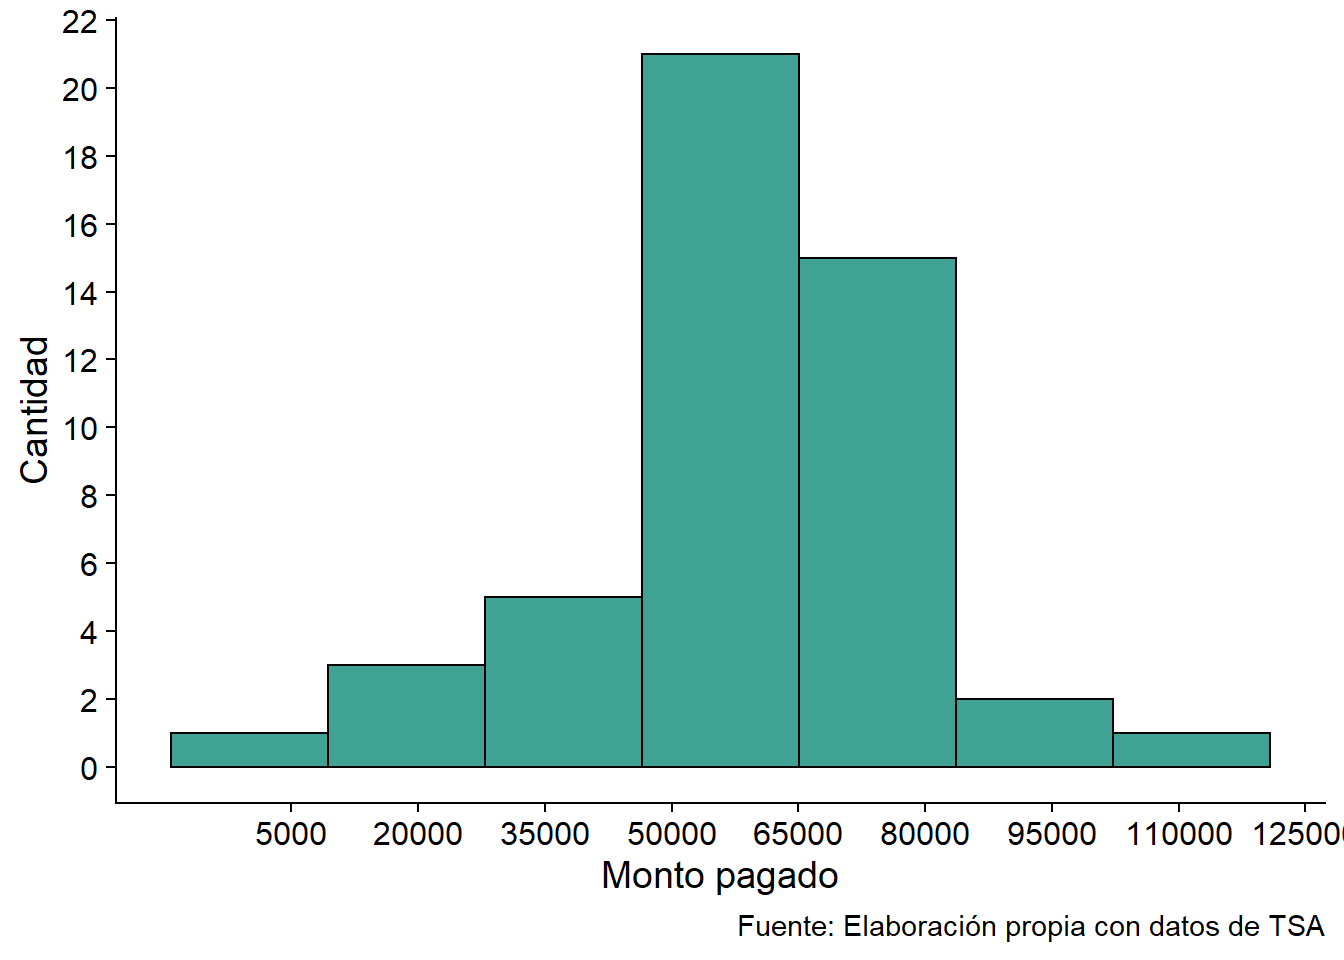
\includegraphics{./Bit2_files/figure-pdf/fig-histograma_severidad-1.pdf}

}

\end{figure}

En la Tabla~\ref{tbl-medidas_severidad_frecuencia} se muestran algunas
estadísticas de los datos de frecuencia y severidad. Sorprende
principalmente la asimetría obtenida para la severidad, que marca una
discrepancia con los resultados obtenidos tanto por Flores (2022) como
por Chen (2020), dado que ambos autores presentan coeficientes de
asimetría positivos, sin embargo, debe tenerse en cuenta que el primero
utiliza datos del período 2003-2015 (desagregados además por sitio y
tipo) y el segundo del período 2008-2012. De la
Figura~\ref{fig-histograma_severidad} ya se observaba que no hay una
asimetría positiva marcada en la severidad.

\hypertarget{tbl-medidas_severidad_frecuencia}{}
\begin{table}
\caption{\label{tbl-medidas_severidad_frecuencia}Medidas estadísticas de resumen para la severidad y la frecuencia }\tabularnewline

\centering
\begin{tabular}[t]{>{}l|>{\raggedleft\arraybackslash}p{2cm}|>{\raggedleft\arraybackslash}p{2cm}}
\hline
\textbf{ } & \textbf{Frecuencia} & \textbf{Severidad}\\
\hline
\textbf{Mínimo} & 44.00 & 9007.07\\
\hline
\textbf{Primer cuartil} & 237.75 & 50883.81\\
\hline
\textbf{Mediana} & 286.00 & 59722.03\\
\hline
\textbf{Media} & 265.48 & 58393.64\\
\hline
\textbf{Tercer cuartil} & 310.00 & 70566.03\\
\hline
\textbf{Máximo} & 396.00 & 120512.60\\
\hline
\textbf{Desviación estándar} & 75.62 & 20787.52\\
\hline
\textbf{Rango intercuartil} & 72.25 & 19682.22\\
\hline
\textbf{Asimetría} & -1.35 & -0.21\\
\hline
\textbf{Curtosis} & 1.73 & 1.21\\
\hline
\end{tabular}
\end{table}

En la tabla Tabla~\ref{tbl-severidadpromedio} se observa la severidad
promedio por mes codificado como 1 para enero y 12 para diciembre. Se
nota que la severidad la relaciona cercanamente con las temporadas
altas: severidades más altas en verano del hemisferio norte y Enero.
Aparte de eso, la severidad es aproximadamente uniforme en el resto de
los meses. 6

\hypertarget{tbl-severidadpromedio}{}
\begin{table}
\caption{\label{tbl-severidadpromedio}Severidad promedio mensual }\tabularnewline

\centering
\begin{tabular}{r|r}
\hline
Mes & Severidad promedio\\
\hline
1 & 72304.02\\
\hline
2 & 50842.60\\
\hline
3 & 66050.08\\
\hline
4 & 58276.72\\
\hline
5 & 59759.59\\
\hline
6 & 62022.79\\
\hline
7 & 62882.68\\
\hline
8 & 65855.69\\
\hline
9 & 52256.92\\
\hline
10 & 55727.93\\
\hline
11 & 49131.62\\
\hline
12 & 45612.98\\
\hline
\end{tabular}
\end{table}

En la Tabla~\ref{tbl-tiporeclamo} se observa que los dos reclamos
desproporcionalmente más frecuentes son los de pérdidas y daños a la
propiedad de los pasajeros.

\hypertarget{tbl-tiporeclamo}{}
\begin{table}
\caption{\label{tbl-tiporeclamo}Frecuencia por tipo de reclamo }\tabularnewline

\centering
\begin{tabular}{l|r}
\hline
Tipo de reclamo & Ocurrencias\\
\hline
- & 212\\
\hline
Bus Terminal & 1\\
\hline
Complaint & 11\\
\hline
Employee Loss (MPCECA) & 18\\
\hline
Motor Vehicle & 143\\
\hline
Passenger Property Loss & 25898\\
\hline
Personal Injury & 383\\
\hline
Property Damage & 14927\\
\hline
Wrongful Death & 4\\
\hline
NA & 1\\
\hline
\end{tabular}
\end{table}

En Tabla~\ref{tbl-aerolinea} Se observa el número de ocurrencias por
aerolínea, esto es, el cantidad de reclamos según la aerolínea en la que
viajaba la persona que realizó el reclamo. Se tiene que la \emph{Delta
Air Lines} es la presenta mayor cantidad de reclamos reportados,
seguidas de \emph{Southwest Airlines} y \emph{American Airlines}, esto
es un comportamiento esperable ya que son aerolíneas líderes de mercado
y por ende presentan mayor cantidad de viajeros y esto influye en la
cantidad de reclamos.

\hypertarget{tbl-aerolinea}{}
\begin{table}
\caption{\label{tbl-aerolinea}Frecuencia de reclamos por aerolínea }\tabularnewline

\centering
\begin{tabular}{l|r}
\hline
Aerolínea  & Ocurrencias\\
\hline
Delta Air Lines & 7029\\
\hline
Southwest Airlines & 5953\\
\hline
American Airlines & 5228\\
\hline
UAL & 4636\\
\hline
USAir & 3055\\
\hline
Jet Blue & 1970\\
\hline
Continental Airlines & 1713\\
\hline
Alaska Airlines & 1505\\
\hline
AirTran Airlines & 1020\\
\hline
British Airways & 596\\
\hline
\end{tabular}
\end{table}

La Figura~\ref{fig-reclamosmensuales} muestra el conteo de incidencias
menusales entre 2010 y finales del 2013. Se Muestra una tendencia fuerte
de incrementeo hasta el mes 40. Esto se puede explicar a partir de que
el TSA fue creado en el 2002 y durante su período inicial de
funcionamiento se implementaron nuevas prácticas de seguridad en el
aeropuerto por lo que los pasajeros y las autoridades tuvieron un
período de aprendizaje. Luego del mes 40 se observa una fuerte tendencia
de decremento posiblemente porque la población a este punto ya se
acostumbró a las nuevas medidas implementadas. Esta tendencia es
importante notarla pues Flores (2022) comenta que puede dificultar el
proceso de ajustarle una distribución.

\begin{figure}[H]

\caption{\label{fig-reclamosmensuales}Número de reclamos mensuales del
2010 al 2013}

{\centering 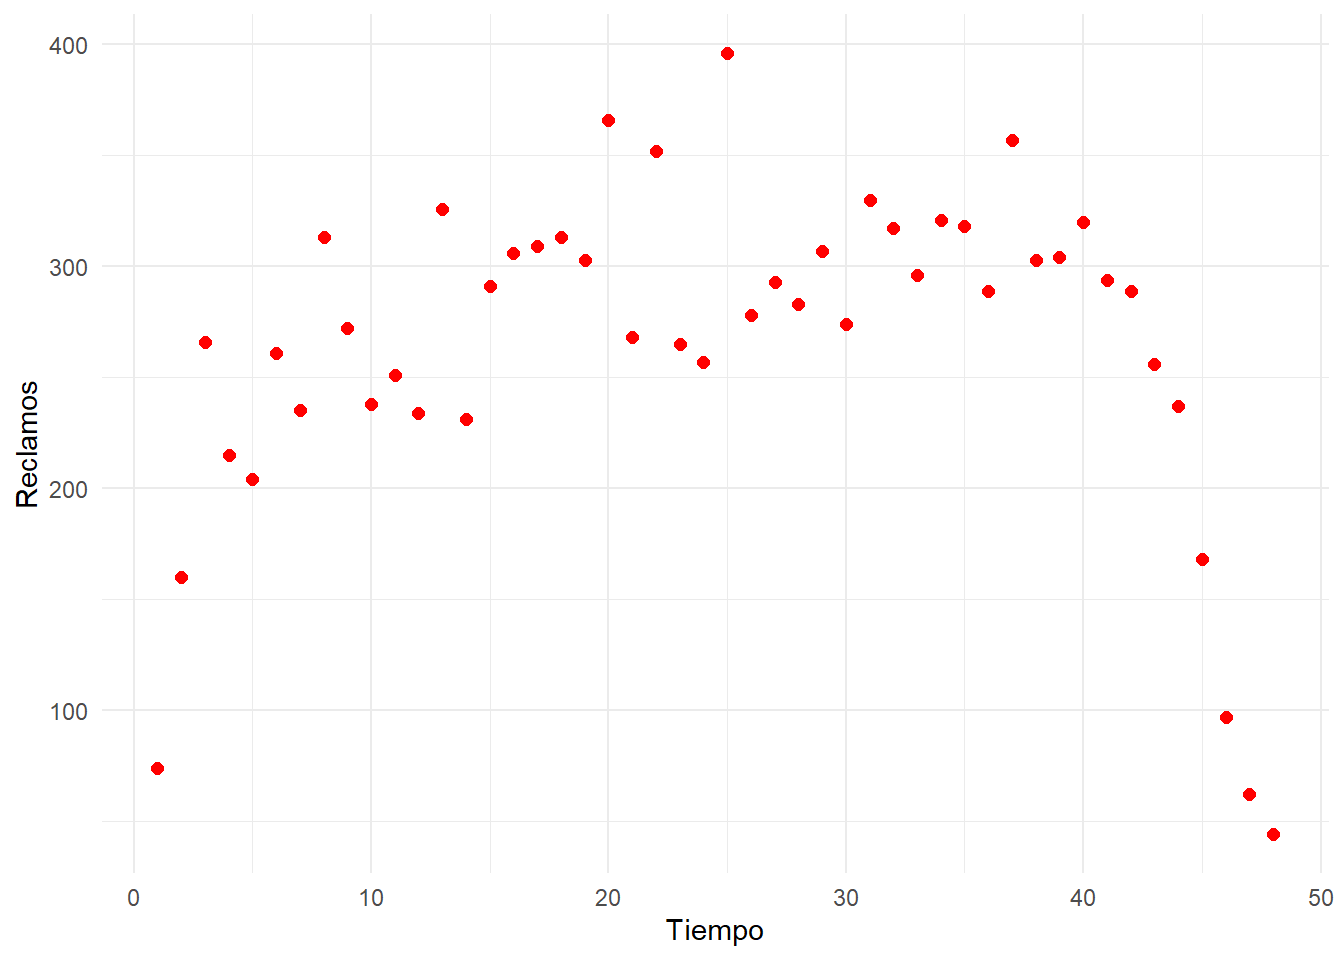
\includegraphics{./Bit2_files/figure-pdf/fig-reclamosmensuales-1.pdf}

}

\end{figure}

\begin{figure}[H]

\caption{\label{fig-mayormontoaerolineas}Aerolíneas con mayor monto
promedio pagado}

{\centering 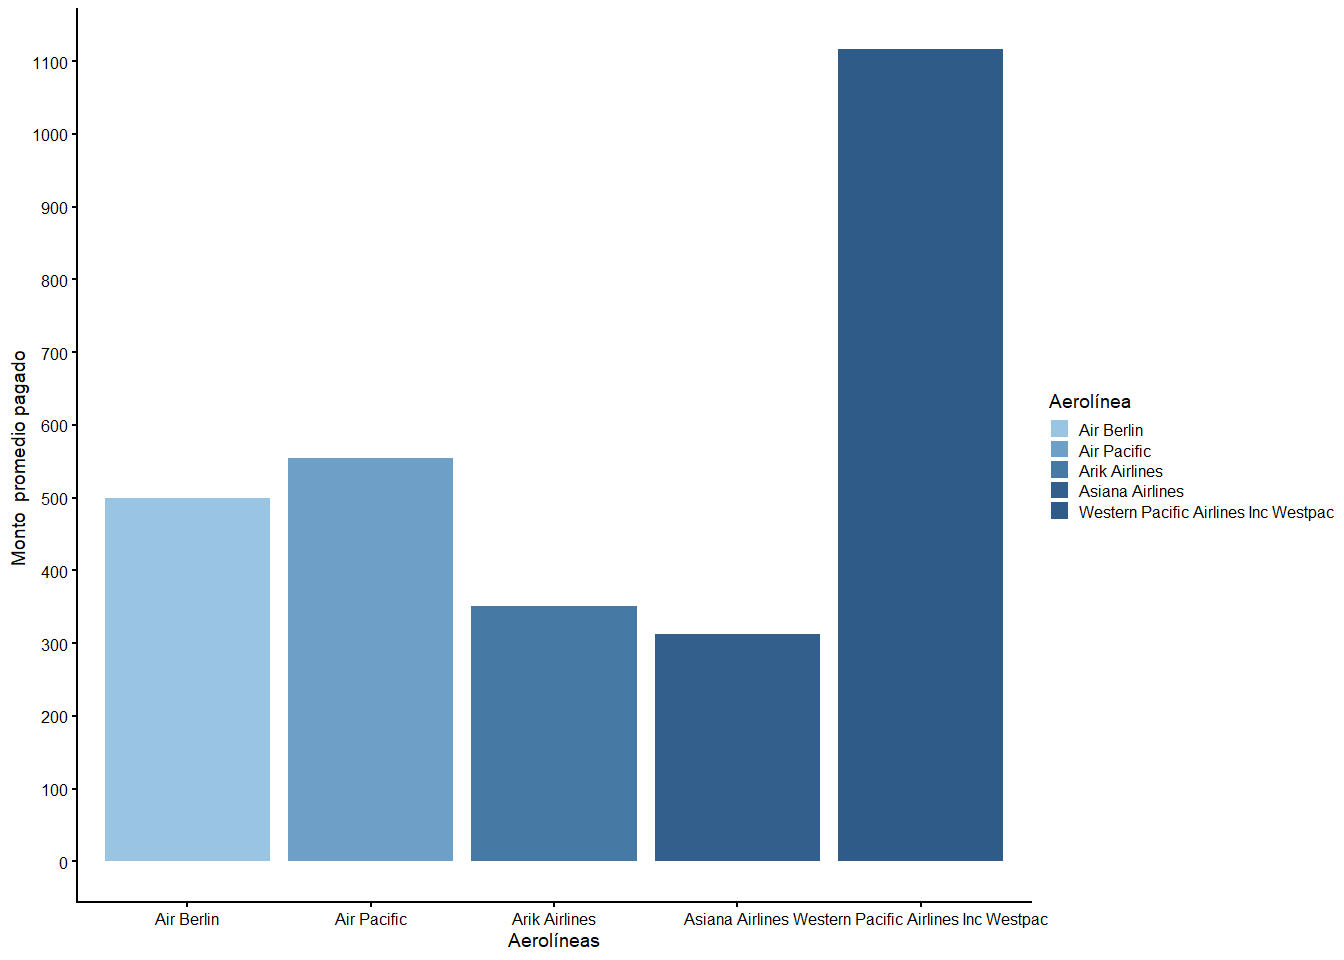
\includegraphics{./Bit2_files/figure-pdf/fig-mayormontoaerolineas-1.pdf}

}

\end{figure}

\begin{verbatim}
Warning: Using `size` aesthetic for lines was deprecated in ggplot2 3.4.0.
i Please use `linewidth` instead.
\end{verbatim}

\begin{figure}[H]

\caption{\label{fig-tiporeclamos}Tipos de reclamos con mayor monto
promedio pagado}

{\centering 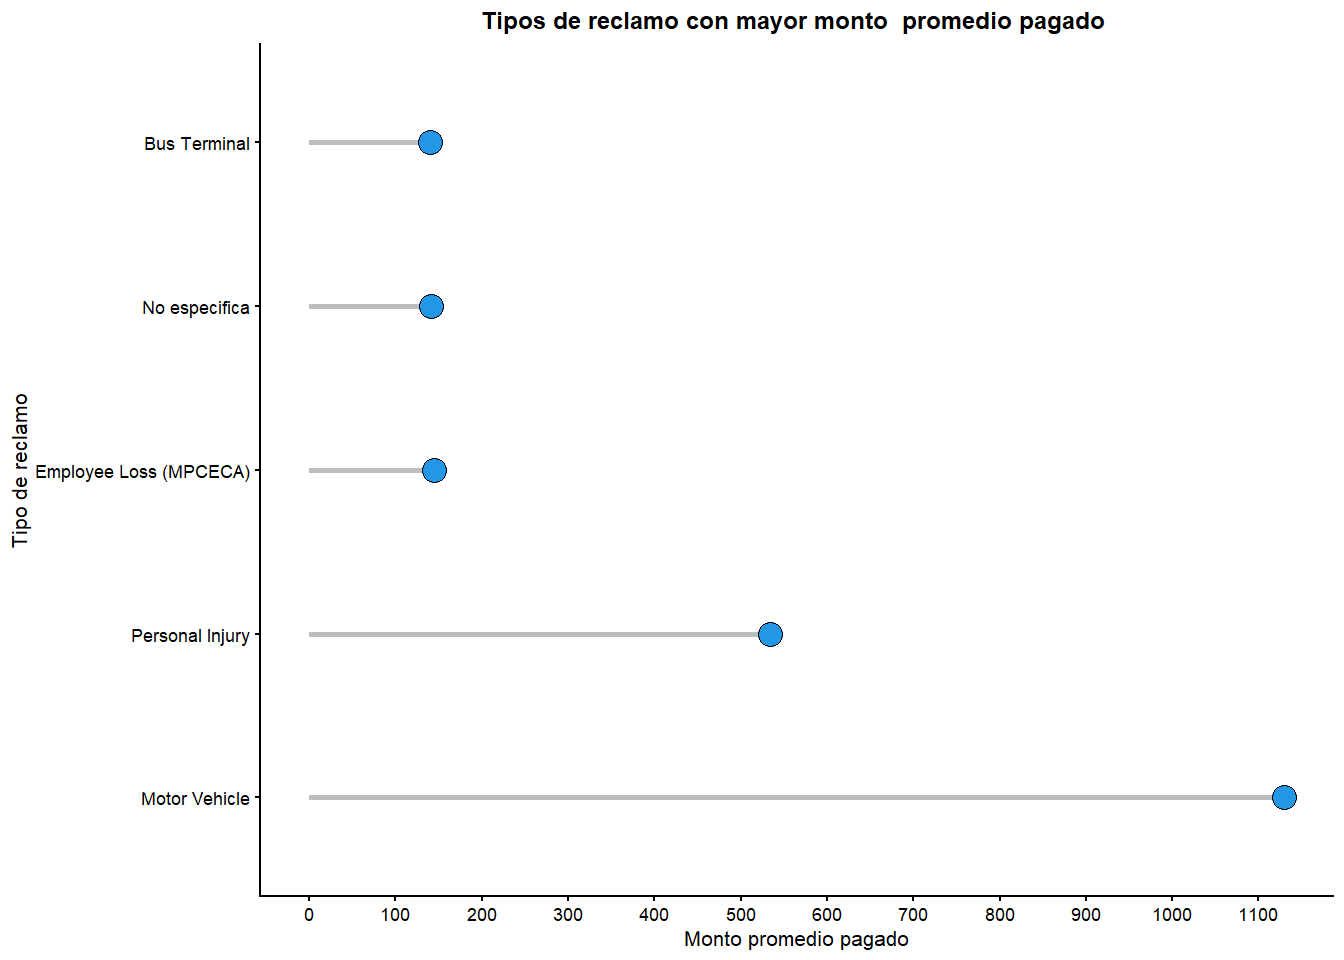
\includegraphics{./Bit2_files/figure-pdf/fig-tiporeclamos-1.pdf}

}

\end{figure}

La Figura~\ref{fig-descdistSeveridad} muestra la relación entre curtosis
y asimetría de severidad agregadas mensualemente. Se observa que
preliminarmente se aproxima a una logística.

\begin{verbatim}
summary statistics
------
min:  9007.07   max:  120512.6 
median:  59722.03 
mean:  58393.64 
estimated sd:  20787.52 
estimated skewness:  -0.2145234 
estimated kurtosis:  4.483542 
\end{verbatim}

\begin{figure}[H]

\caption{\label{fig-descdistSeveridad}Comparación de la curtosis y
asimetría de la severidad}

{\centering 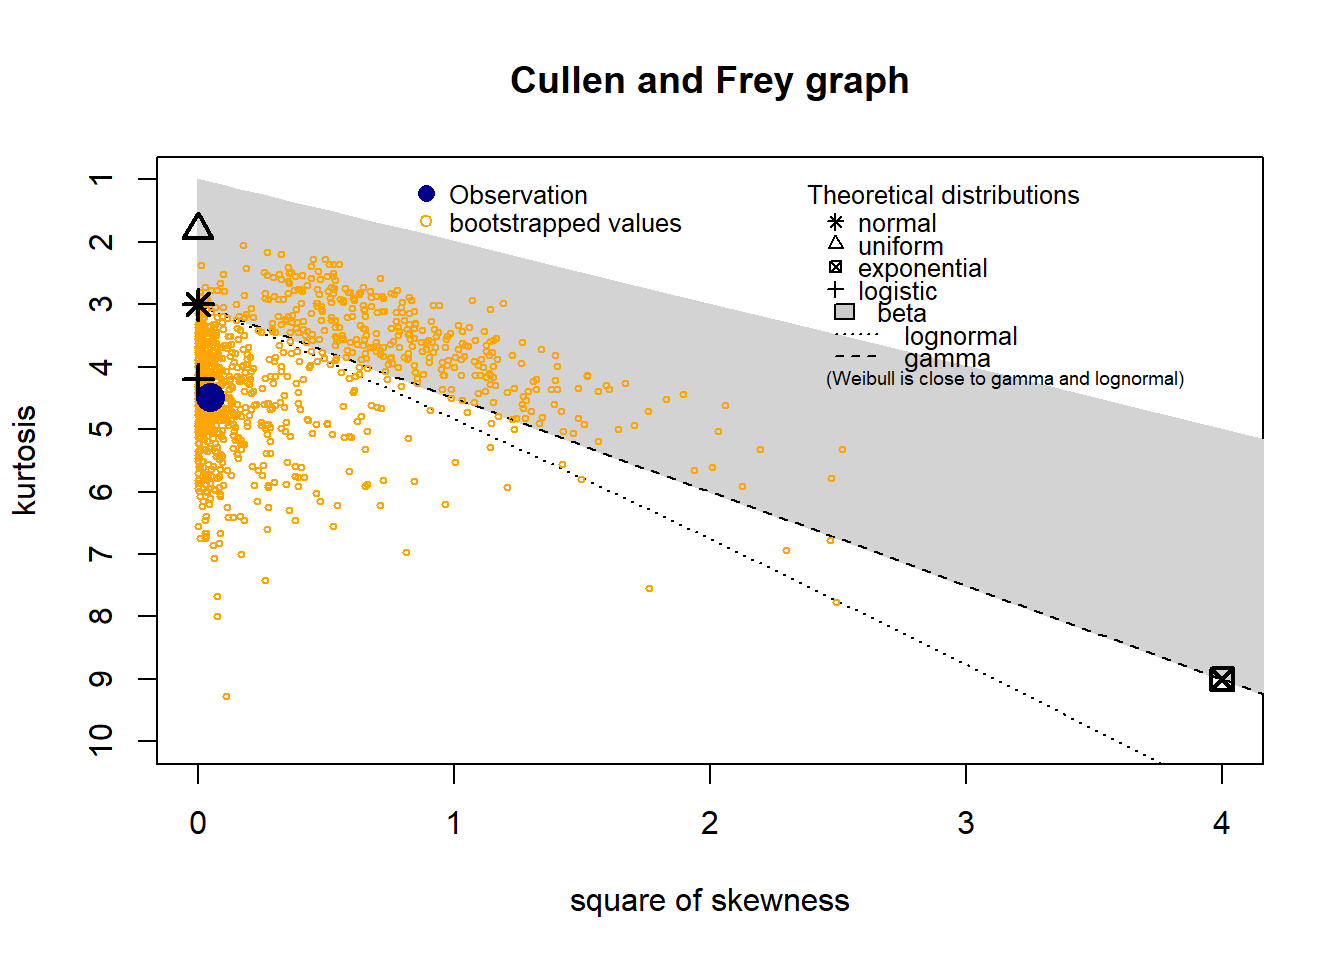
\includegraphics{./Bit2_files/figure-pdf/fig-descdistSeveridad-1.pdf}

}

\end{figure}

\hypertarget{fichas-bibliogruxe1ficas}{%
\section{Fichas Bibliográficas:}\label{fichas-bibliogruxe1ficas}}

1).

\begin{itemize}
\item
  Nombre de su hallazgo/resultado: Tendencia en la ocurrencia de
  reclamos
\item
  Resumen en una oración: El número de reclamos mensuales incrementa con
  respecto al tiempo en los primeros 40 meses hasta alcanzar un máximo y
  desde entonces se ha mostrado un comportamiento a la baja en la
  cantidad de reclamos hechos.
\item
  Principal característica: Tendencia aparente
\item
  Problemas o posibles desafíos: En Flores (2022), se comenta que la
  existencia de una tendencia en los reclamos puede causar problemas al
  momento de buscar las distribuciones que se ajusten a los datos.
\item
  Resumen en un párrafo: El número de reclamos mensuales parece
  incrementar rápidamente en los primeros 40 meses del período
  estudiado. Esto se podría explicar por la poca experiencia en materia
  de chequeos y procedimientos por parte de los pasajeros y las
  autoridades. Luego del mes 40 se observa una tendencia a la baja en la
  cantidad de reclamos, posiblemente porque a este punto ya se habían
  interiorizado las nuevas prácticas de seguridad. Esta tendencia puede
  ser un problema porque en la literatura se expresó que puede complicar
  el proceso de ajustar una distribución a los reclamos, notando que al
  eliminar esta tendencia se facilitaba esta búsqueda.
\end{itemize}

2).

\begin{itemize}
\item
  Nombre de su hallazgo/resultado: Asimetría negativa de la severidad
\item
  Resumen en una oración: La distribución de la severidad está
  ligeramente sesgada hacia la derecha, según lo indica un valor
  negativo del coeficiente de asimetría.
\item
  Principal característica: El coeficiente de asimetría es negativo.
\item
  Problemas o posibles desafíos: Esta característica es contrastante
  respecto de los resultados obtenidos por autores que han utilizado
  datos de reclamos a TSA, donde la asimetría positiva era muy marcada
  tanto numérica como visualmente y probalemente signifique que las
  distribuciones a emplear en el presente trabajo para ajustar la
  severidad sean muy distintas de las ya estudiadas.
\item
  Resumen en un párrafo: La distribución de la severidad está
  ligeramente sesgada hacia la derecha, según lo indica un valor bajo
  pero negativo del coeficiente de asimetría en la
  Tabla~\ref{tbl-medidas_severidad_frecuencia}. Del histograma en la
  Figura~\ref{fig-histograma_severidad} ya se observaba que la
  distribución de la severidad agregada por mes no es claramente sesgada
  hacia la izquierda. Esta característica sorprende y marca una
  diferencia notable respecto de los resultados obtenidos por autores
  que han utilizado datos de reclamos a TSA, como en los trabajos de
  Flores (2022) y Chen (2020), donde la asimetría positiva era muy
  marcada tanto numérica como visualmente y probalemente signifique que
  las distribuciones a emplear en el presente trabajo para ajustar la
  severidad sean muy distintas de las ya estudiadas.
\end{itemize}

3).

\begin{itemize}
\item
  Nombre de su hallazgo/resultado: Variables de estudio secundarias con
  mayor monto promedio pagado.
\item
  Resumen en una oración: Existen variables secundarias de nuestros
  estudio que tienen alto impacto implícito en la severidad de los
  montos promedio pagados, estas son:tipo de reclamo y aerolíneas. Donde
  el tipo de reclamo con mayor monto promedio es \emph{motor vehicule} y
  para el caso de la aerolínea es \emph{Western Pacific Airlines Inc
  Westpac}.
\item
  Principal característica:Pese a que las variables principales para
  nuestro estudio son la frecuencia de reclamos y la severidad de estos.
  Existen variables secundarias que implícitamente tienen alto impacto
  en las mencionadas variables principales.
\item
  Problemas o posibles desafíos:Existen observaciones donde no se
  reporta tanto la aerolínea como el tipo de reclamo por lo que solo se
  contemplan para el monto promedio de pago aquellas observaciones donde
  si se registran la información de las variables tipo de reclamo y
  aerolínea.
\item
  Resumen en un párrafo:
\end{itemize}

Hay en particular dos variables secundarias altamente ligadas a la
severidad para nuestro estudio, estas variables son: Tipo de reclamo y
la aerolínea en la que viajaba la persona.

Es importante saber cuales son aquellos tipos de reclamo con mayor monto
promedio pagado, como se observa en el Figura~\ref{fig-tiporeclamos}, el
reclamo por \emph{motor vehicule} y \emph{personal injury} son aquellos
que presentan mayor severidad, seguido de un subgrupo donde el monto de
reclamo es menor como lo son: \emph{employee loss} y \emph{bus
terminal}.

Análogamente, para el caso de las aerolíneas a las que pertenecen las
personas que reportan mayor monto promedio pagado, se observa en el
Figura~\ref{fig-mayormontoaerolineas} que \emph{Western Pacific Airlines
Inc Westpac} es la que presenta mayor monto promedio, seguido de
\emph{Air Pacific}.

\hypertarget{parte-de-reflexiuxf3n}{%
\section{Parte de reflexión}\label{parte-de-reflexiuxf3n}}

En la Figura~\ref{fig-UVE2} se muestra la UVE heurística actualizada,
donde se incluyen las transformaciones sobre los datos para obtener los
datos mensuales de frecuencia y severidad.

\begin{figure}[H]

\caption{\label{fig-UVE2}Actualización de de la UVE Heurística}

{\centering 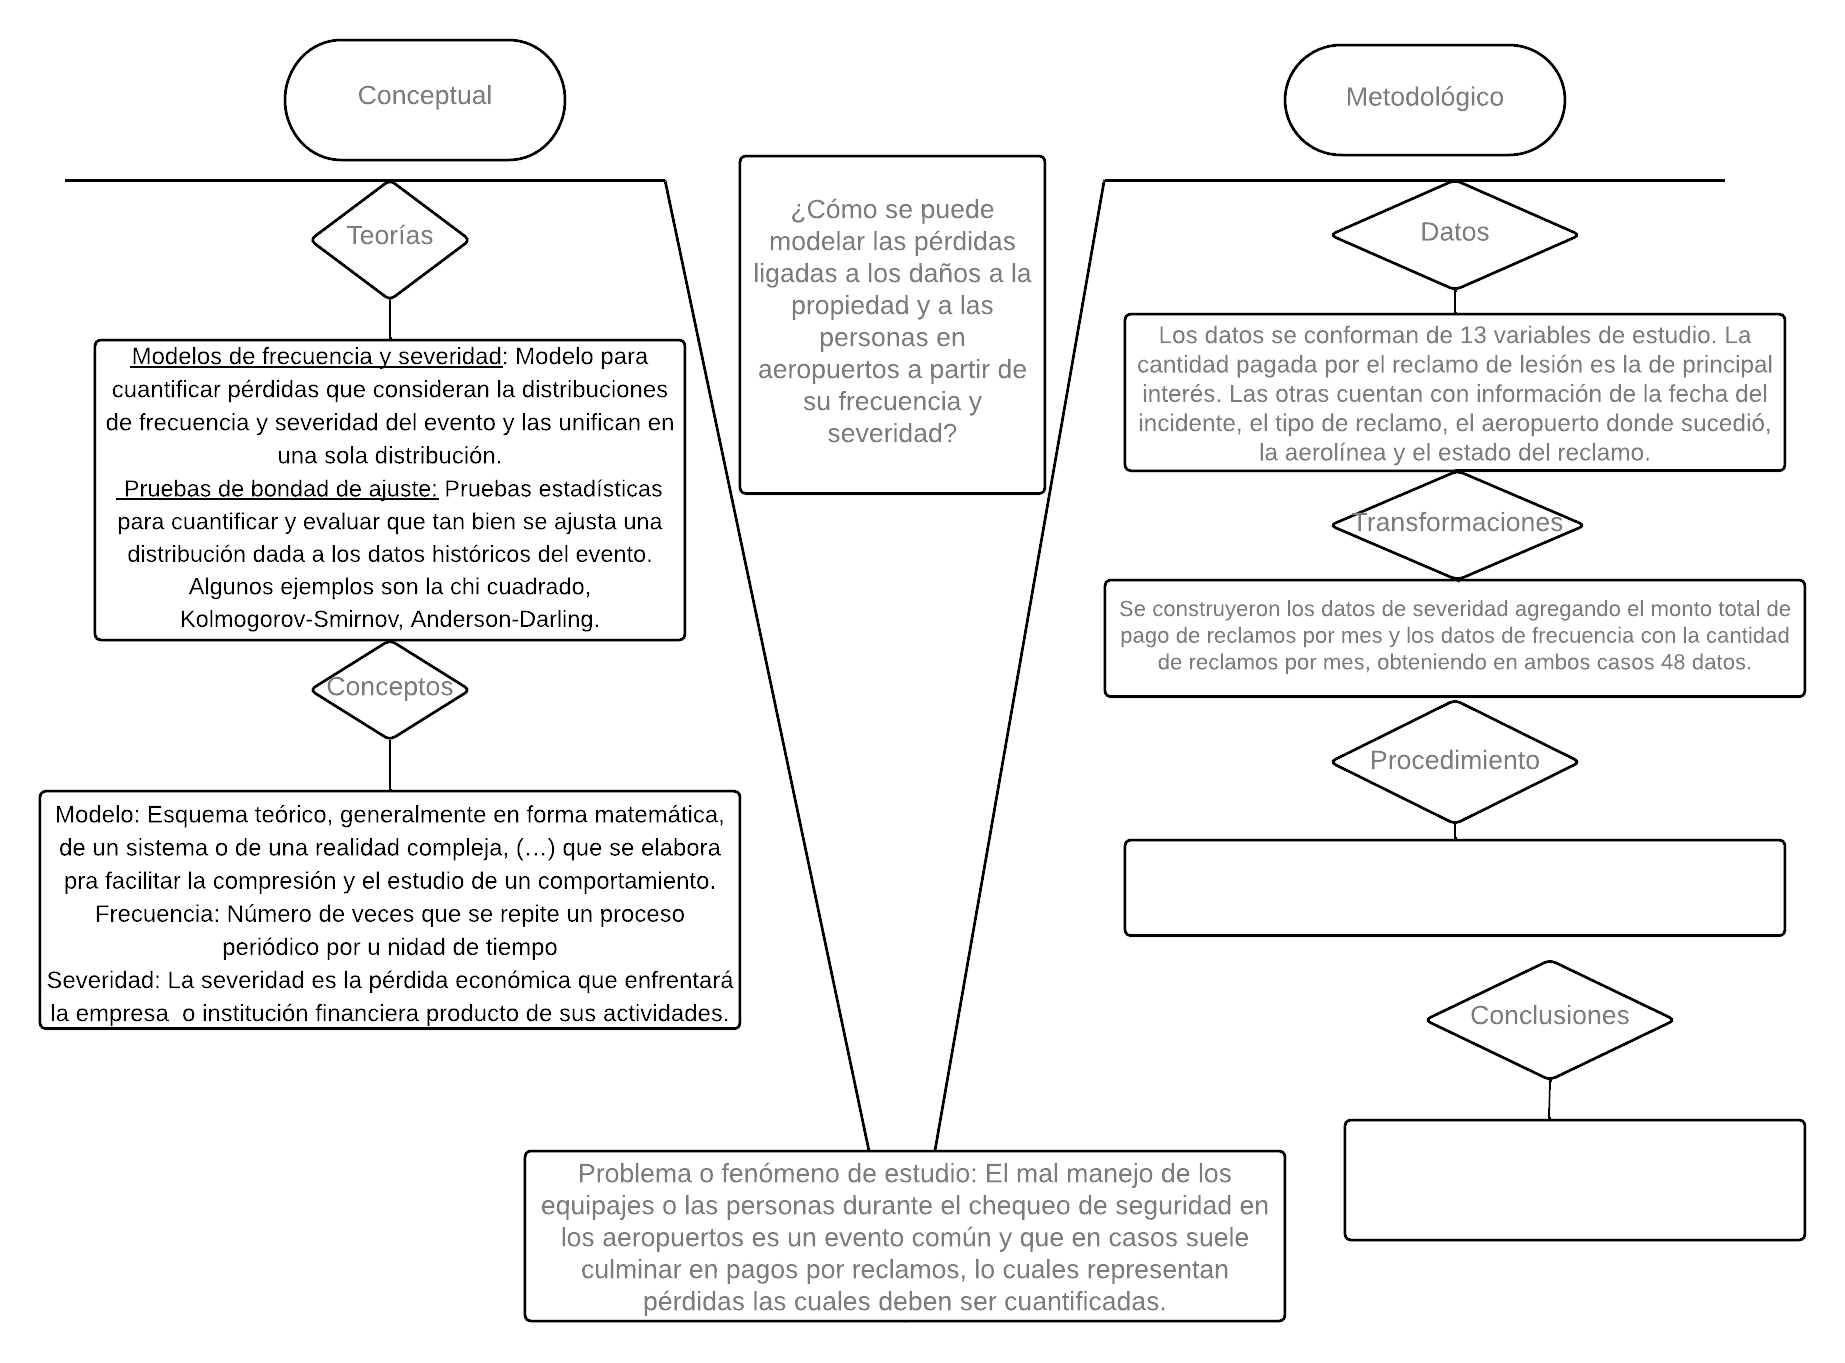
\includegraphics[width=6.25in,height=\textheight]{./Images/UVE Maik 2.png}

}

\end{figure}

En cuanto a las preguntas surgidas, sin duda el punto más sorpresivo
consiste en la discordancia de la asimetría hallada para la distribución
empírica de la severidad en contraste con los resultados expuestos por
Flores (2022) y Chen (2020), quienes realizaron la agregación de la
severidad de forma mensual y trabajaron con datos de reclamos a TSA pero
para periodos distintos, hallando una marcada asimetría positiva. De
esta manera, surge la duda de a qué puede obedecer esta diferencia,
aunque debe tenerse en cuenta que contestar esta pregunta no es el
objetivo de la presente investigación.

\bookmarksetup{startatroot}

\hypertarget{bituxe1cora-3}{%
\chapter{Bitácora 3}\label{bituxe1cora-3}}

\hypertarget{parte-de-planificaciuxf3n-1}{%
\section{Parte de Planificación}\label{parte-de-planificaciuxf3n-1}}

\hypertarget{ajuste-de-la-frecuencia}{%
\subsection{Ajuste de la frecuencia}\label{ajuste-de-la-frecuencia}}

En la Figura~\ref{fig-ajustePoisson} se muestra el ajuste de la
distribución Poisson, y su versión truncada y modificada en cero, donde
se comprueba que estas no difieren mucho entre sí, aparte de que se
observa que el ajuste no es bueno.

\begin{figure}[H]

\caption{\label{fig-ajustePoisson}Ajustes distribución Poisson}

{\centering 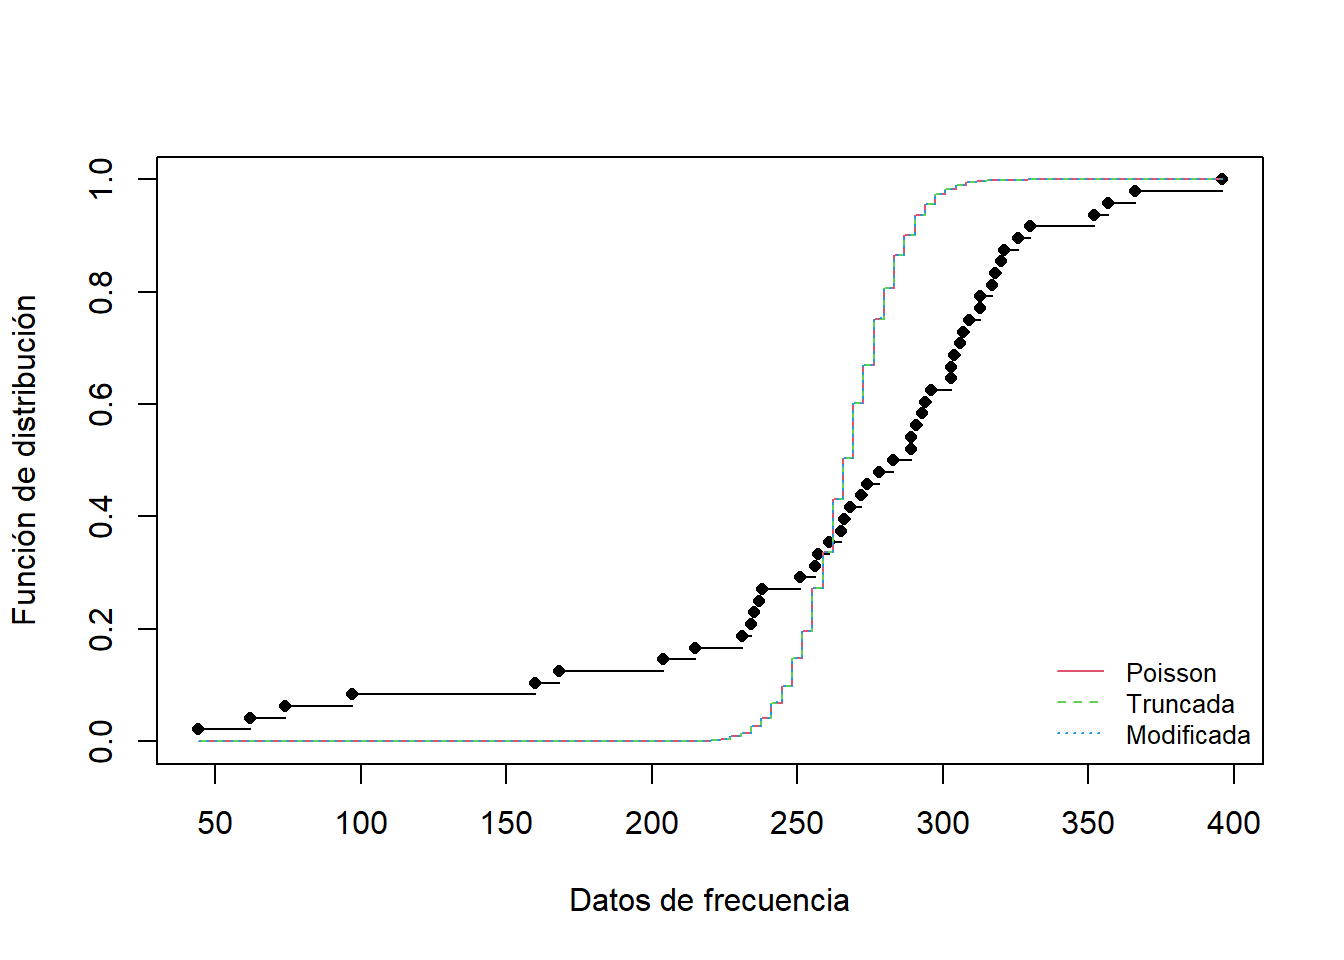
\includegraphics{./Bit3_files/figure-pdf/fig-ajustePoisson-1.pdf}

}

\end{figure}

En la Figura~\ref{fig-ajustebinneg} se muestra el ajuste de la
distribución binomial negativa, y su versión truncada y modificada en
cero, donde se comprueba que estas no difieren mucho entre sí, aparte de
que se observa que el ajuste es un poco mejor que el de la Poisson, sin
llegar a ser satisfactorio.

\begin{figure}[H]

\caption{\label{fig-ajustebinneg}Ajustes distribución binomial negativa}

{\centering 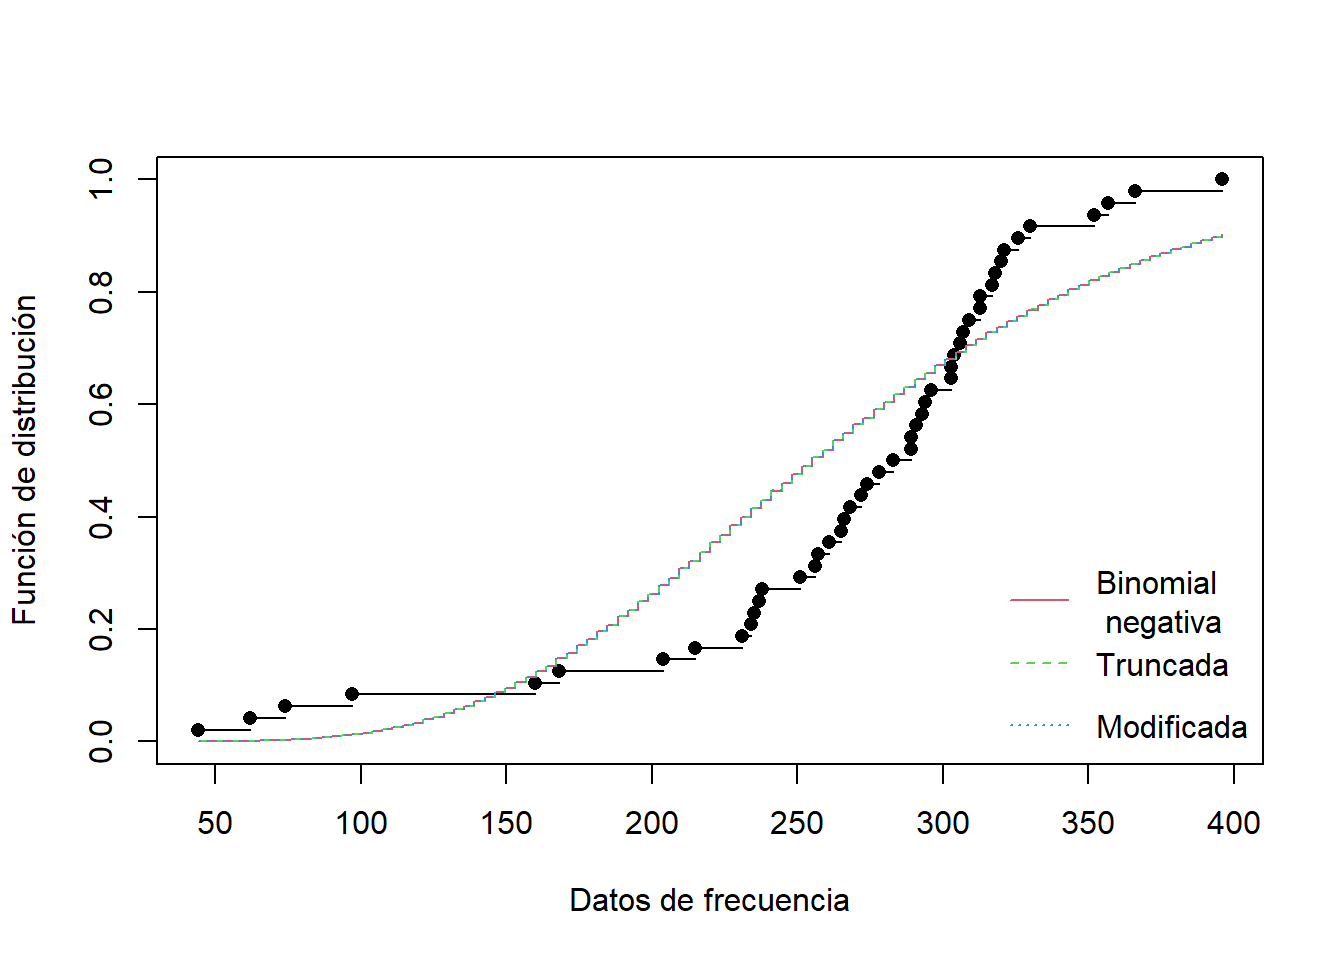
\includegraphics{./Bit3_files/figure-pdf/fig-ajustebinneg-1.pdf}

}

\end{figure}

En la Figura~\ref{fig-ajustegeom} se muestra el ajuste de la
distribución geométrica, y su versión truncada y modificada en cero,
donde se comprueba que estas no se diferencian mucho. Siendo esta
distribución un caso particular de la binomial negativa, se ve que el
ajuste es muy inferior al del caso general. No es claro si el ajuste de
la geométrica es mejor al de la Poisson.

\begin{figure}[H]

\caption{\label{fig-ajustegeom}Ajustes distribución geométrica}

{\centering 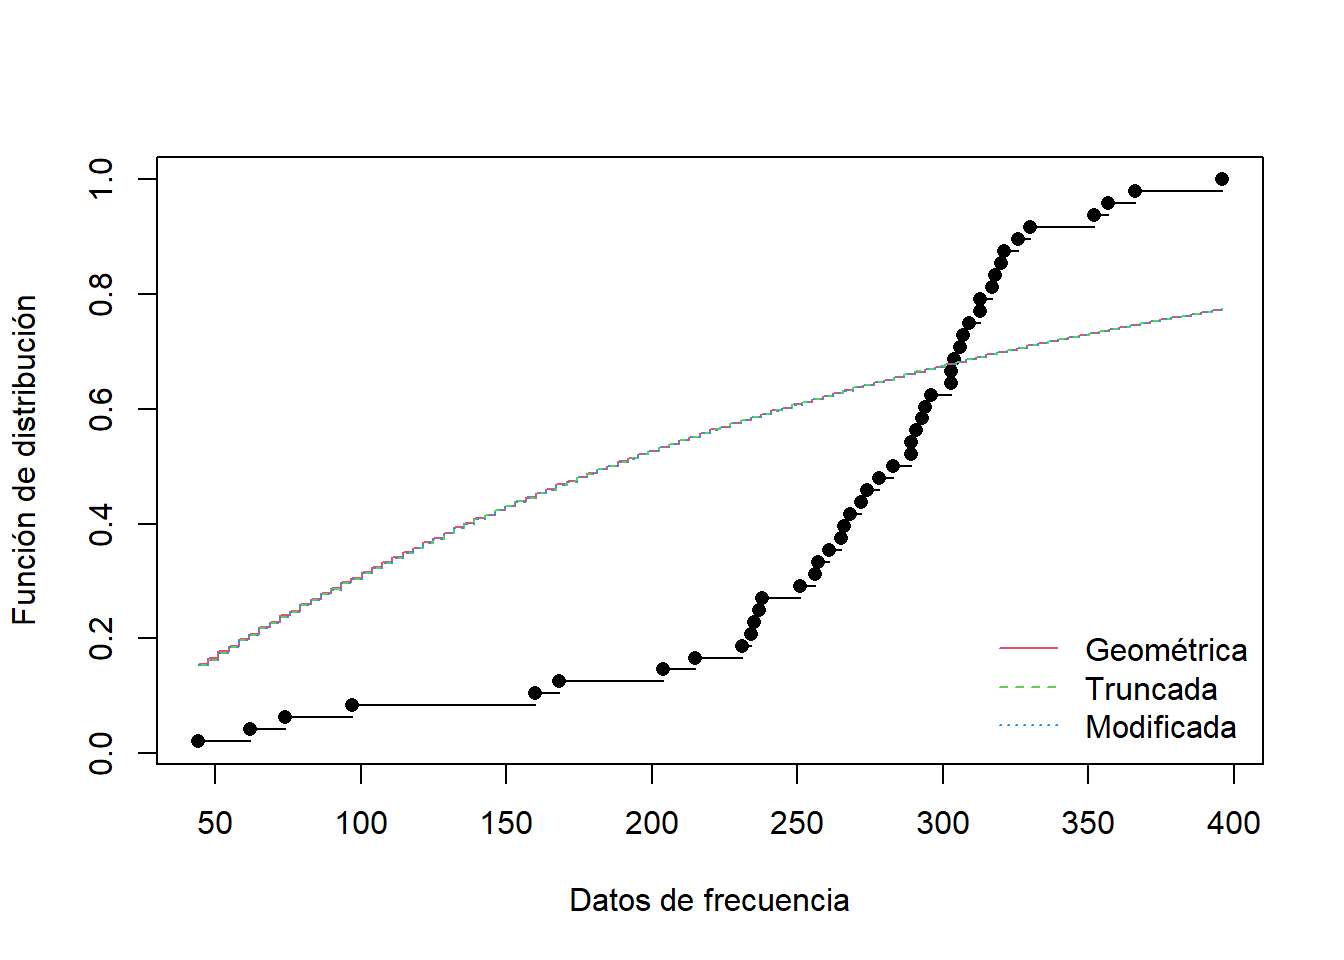
\includegraphics{./Bit3_files/figure-pdf/fig-ajustegeom-1.pdf}

}

\end{figure}

A continuación, en la Figura~\ref{fig-ajustebinom}, se presenta el
ajuste de la distribución binomial, el cual luce similar al de la
Poisson y se ve que no es muy bueno.

\begin{figure}[H]

\caption{\label{fig-ajustebinom}Ajustes distribución binomial}

{\centering 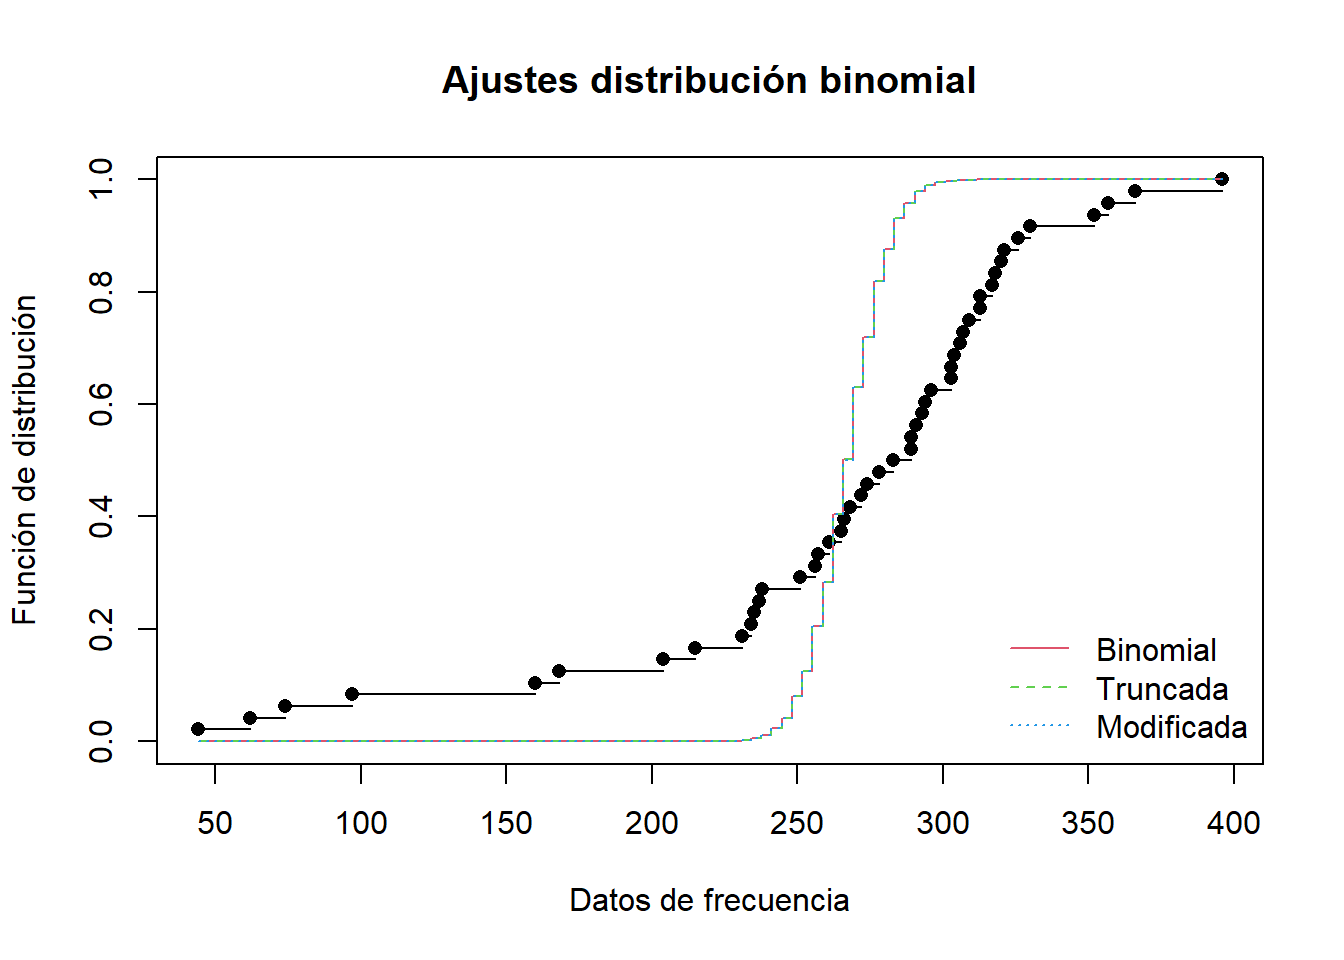
\includegraphics{./Bit3_files/figure-pdf/fig-ajustebinom-1.pdf}

}

\end{figure}

En la Figura~\ref{fig-ajusteab0} se muestran todos los ajustes de las
distribuciones de la clase \((a,b,0)\), lo que permite comparar y ver
que la binomial negativa es la que mejor emula el comportamiento de la
dsitribución empírica de los datos, estado, sin embargo, lejos de ser
adecuado.

\begin{figure}[H]

\caption{\label{fig-ajusteab0}Ajustes con distribuciones de la clase
(a,b,0)}

{\centering 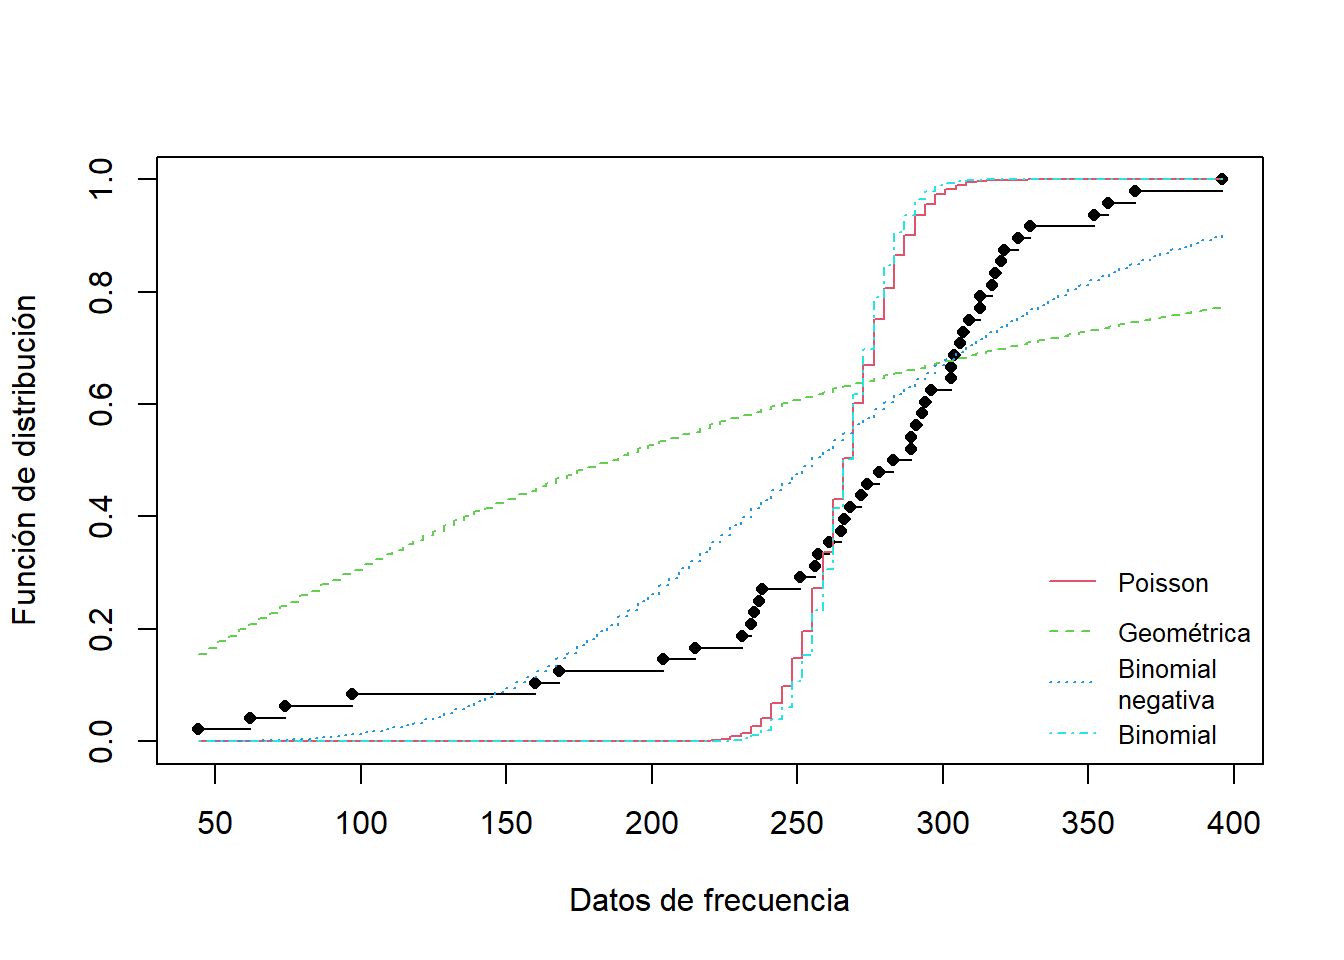
\includegraphics{./Bit3_files/figure-pdf/fig-ajusteab0-1.pdf}

}

\end{figure}

A su vez, en la Figura~\ref{fig-ajusteab1trunc} están los miembros de la
clase \((a,b,1)\) truncadas en cero, los cuáles no muestran ser mejores
que sus distribuciones originales en la clase \((a,b,0)\).

\begin{figure}[H]

\caption{\label{fig-ajusteab1trunc}Ajustes con distribuciones de la
clase (a,b,1) truncadas en cero}

{\centering 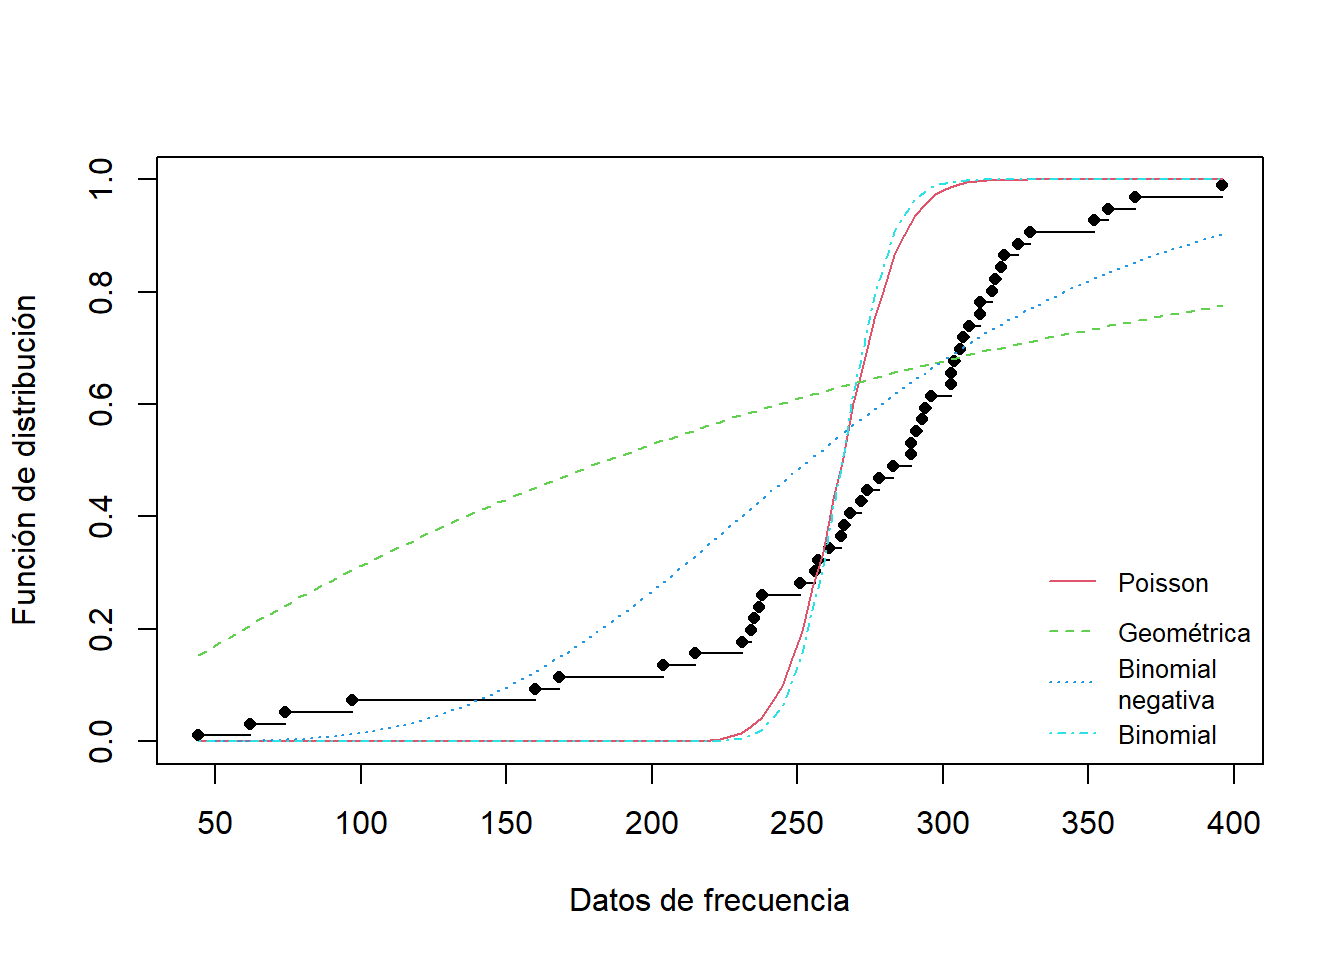
\includegraphics{./Bit3_files/figure-pdf/fig-ajusteab1trunc-1.pdf}

}

\end{figure}

A su vez, en la Figura~\ref{fig-ajusteab1mod} están los miembros de la
clase \((a,b,1)\) modificadas en cero, los cuáles tampoco son
visiblemente mejores que sus distribuciones originales en la clase
\((a,b,0)\).

\begin{figure}[H]

\caption{\label{fig-ajusteab1mod}Ajustes con distribuciones de la clase
(a,b,1) modificadas en cero}

{\centering 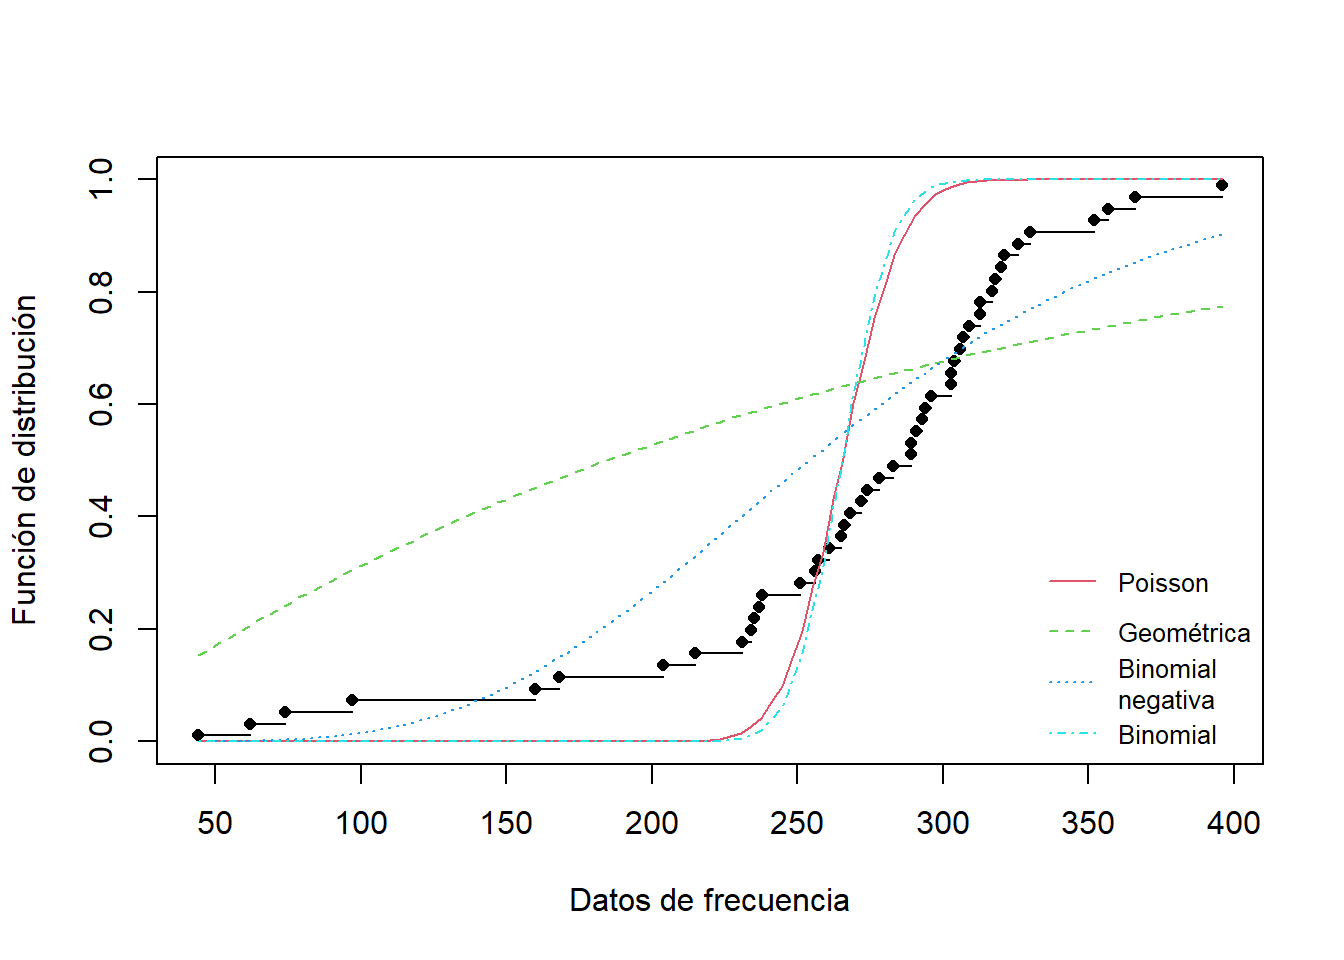
\includegraphics{./Bit3_files/figure-pdf/fig-ajusteab1mod-1.pdf}

}

\end{figure}

\hypertarget{tbl-parametrosFrecuencia}{}
\begin{table}
\caption{\label{tbl-parametrosFrecuencia}Parámetros de los modelos ajustados para la frecuencia }\tabularnewline

\centering
\begin{tabular}{l|l}
\hline
\textbf{$\textbf{Distribución}$} & \textbf{$\textbf{Parámetros en } \texttt{R}$}\\
\hline
\cellcolor{gray!6}{Poisson} & \cellcolor{gray!6}{$\texttt{ lambda }$ = 265.479167}\\
\hline
ZT-Poisson & $\texttt{ lambda }$ = 265.479326\\
\hline
\cellcolor{gray!6}{ZM-Poisson} & \cellcolor{gray!6}{$\texttt{ lambda }$ = 265.473341 , $\texttt{ p0 }$ = 0}\\
\hline
Binomial negativa & $\texttt{ size }$ = 7.764187 , $\texttt{ mu }$ = 265.491586\\
\hline
\cellcolor{gray!6}{ZT-Binomial negativa} & \cellcolor{gray!6}{$\texttt{ size }$ = 7.762927 , $\texttt{ prob }$ = 0.028412}\\
\hline
ZM-Binomial negativa & $\texttt{ size }$ = 7.759127 , $\texttt{ prob }$ = 0.028396 , $\texttt{ p0 }$ = 0\\
\hline
\cellcolor{gray!6}{Geométrica} & \cellcolor{gray!6}{$\texttt{ prob }$ = 0.003753}\\
\hline
ZT-Geométrica & $\texttt{ prob }$ = 0.003768\\
\hline
\cellcolor{gray!6}{ZM-Geométrica} & \cellcolor{gray!6}{$\texttt{ prob }$ = 0.003766 , $\texttt{ p0 }$ = 0}\\
\hline
Binomial & $\texttt{ prob }$ = 0.29629 , $\texttt{ size }$ = 896\\
\hline
\cellcolor{gray!6}{ZT-Binomial} & \cellcolor{gray!6}{$\texttt{ prob }$ = 0.29629 , $\texttt{ size }$ = 896}\\
\hline
ZM-Binomial & $\texttt{ prob }$ = 0.296296 , $\texttt{ size }$ = 896 , $\texttt{ p0 }$ = 0\\
\hline
\end{tabular}
\end{table}

\hypertarget{tbl-metricasFrecuencia}{}
\begin{table}
\caption{\label{tbl-metricasFrecuencia}Métricas de los modelos ajustados para la frecuencia }\tabularnewline

\centering
\begin{tabular}{l|l|l|l}
\hline
\textbf{Distribución} & \textbf{AIC} & \textbf{BIC} & \textbf{Valor $p$}\\
\hline
\cellcolor{gray!6}{Poisson} & \cellcolor{gray!6}{1617.17955289} & \cellcolor{gray!6}{1619.0507539} & \cellcolor{gray!6}{0}\\
\hline
ZT-Poisson & 1617.1795529 & 1619.05075391 & 0\\
\hline
\cellcolor{gray!6}{ZM-Poisson} & \cellcolor{gray!6}{1619.17955922} & \cellcolor{gray!6}{1622.92196124} & \cellcolor{gray!6}{0}\\
\hline
Binomial negativa & 575.35774711 & 579.10014913 & 3.5478e-06\\
\hline
\cellcolor{gray!6}{ZT-Binomial negativa} & \cellcolor{gray!6}{575.35774432} & \cellcolor{gray!6}{579.10014634} & \cellcolor{gray!6}{3.5344e-06}\\
\hline
ZM-Binomial negativa & 577.35774424 & 582.97134727 & 1.1145e-06\\
\hline
\cellcolor{gray!6}{Geométrica} & \cellcolor{gray!6}{634.00807001} & \cellcolor{gray!6}{635.87927102} & \cellcolor{gray!6}{0}\\
\hline
ZT-Geométrica & 633.64646075 & 635.51766176 & 0\\
\hline
\cellcolor{gray!6}{ZM-Geométrica} & \cellcolor{gray!6}{635.64646629} & \cellcolor{gray!6}{639.38886831} & \cellcolor{gray!6}{0}\\
\hline
Binomial & 2009.5128356 & 2013.25523762 & 0\\
\hline
\cellcolor{gray!6}{ZT-Binomial} & \cellcolor{gray!6}{2009.5128356} & \cellcolor{gray!6}{2013.25523762} & \cellcolor{gray!6}{0}\\
\hline
ZM-Binomial & 2011.51283388 & 2017.12643691 & 0\\
\hline
\end{tabular}
\end{table}

\hypertarget{ajuste-de-la-severidad}{%
\subsection{Ajuste de la severidad}\label{ajuste-de-la-severidad}}

\begin{figure}[H]

\caption{\label{fig-denscompSeveridad}Densidad de las distribuciones
ajustadas con MLE}

{\centering 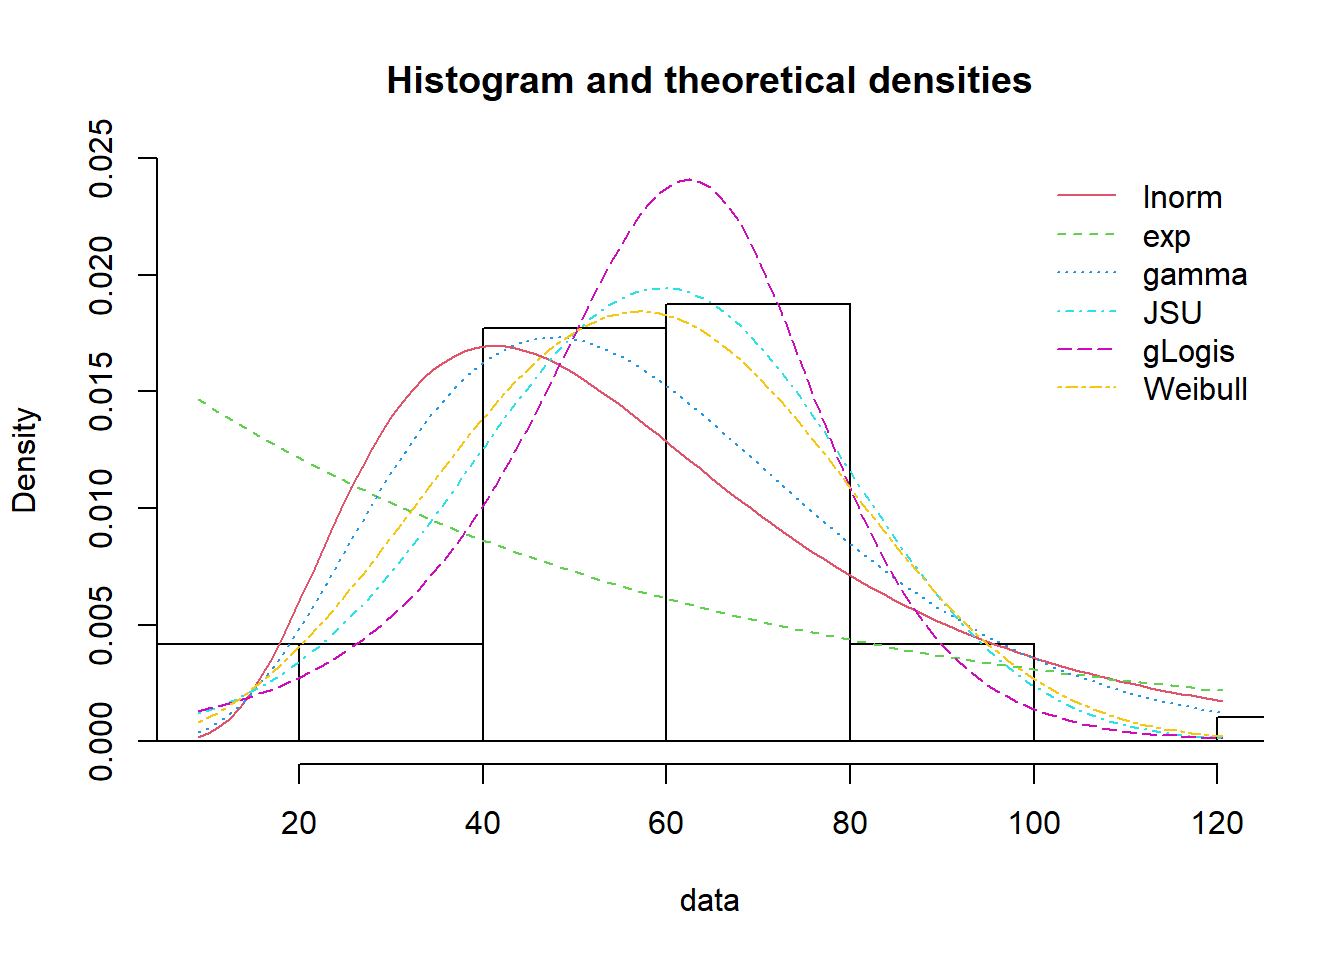
\includegraphics{./Bit3_files/figure-pdf/fig-denscompSeveridad-1.pdf}

}

\end{figure}

La Figura~\ref{fig-denscompSeveridad} muestra que la logística
generalizada, weibull y Johnson SU muestran la forma que acerca más al
histograma. Las otras distribuciones no se aproximan tan bien a los
datos.

\begin{figure}[H]

\caption{\label{fig-cdfcompSeveridad}Función cumulativa de las
distribuciones ajustadas con MLE}

{\centering 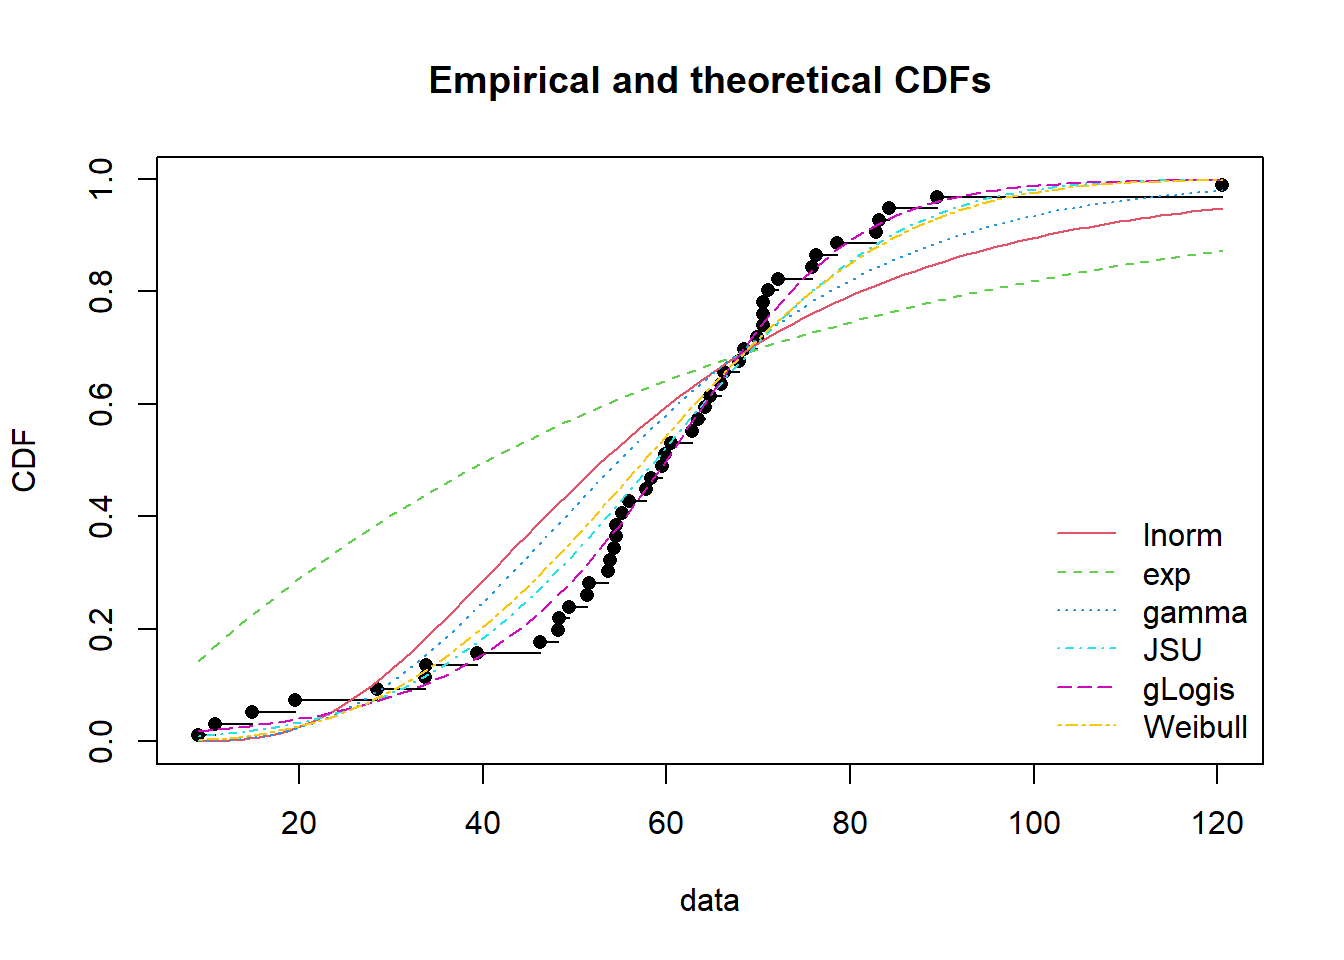
\includegraphics{./Bit3_files/figure-pdf/fig-cdfcompSeveridad-1.pdf}

}

\end{figure}

La Figura~\ref{fig-cdfcompSeveridad} se muestra la distribución
cumulativa, la cual muestra más claramente que las distribuciones
mencionadas anteriormentes se ajustan mejor. En la
Tabla~\ref{tbl-parametrosSeveridad} se muestran los parámetros ajustados
para cada modelo. Se observa que los modelos más adecuados, al menos
visualmente, son más complejos al tener tres y cuatro parámetros

\hypertarget{tbl-parametrosSeveridad}{}
\begin{table}
\caption{\label{tbl-parametrosSeveridad}Parámetros de los modelos ajustados para la severidad }\tabularnewline

\centering
\begin{tabular}{l|l}
\hline
\textbf{$\textbf{Distribución}$} & \textbf{$\textbf{Parámetros en } \texttt{R}$}\\
\hline
\cellcolor{gray!6}{Lognormal} & \cellcolor{gray!6}{$\texttt{ meanlog }$ = 3.972659 , $\texttt{ sdlog }$ = 0.502333}\\
\hline
Exponencial & $\texttt{ rate }$ = 0.017125\\
\hline
\cellcolor{gray!6}{Gamma} & \cellcolor{gray!6}{$\texttt{ shape }$ = 5.448032 , $\texttt{ rate }$ = 0.093297}\\
\hline
SU de Johnson & $\texttt{ mu }$ = 58.400803 , $\texttt{ sigma }$ = 20.541279 , $\texttt{ nu }$ = -31.417414 , $\texttt{ tau }$ = 24.031833\\
\hline
\cellcolor{gray!6}{Logística generalizada} & \cellcolor{gray!6}{$\texttt{ location }$ = 67.038277 , $\texttt{ scale }$ = 8.5276 , $\texttt{ shape }$ = 0.581247}\\
\hline
Weibull & $\texttt{ shape }$ = 3.061525 , $\texttt{ scale }$ = 64.909845\\
\hline
\end{tabular}
\end{table}

\hypertarget{tbl-metricasSeveridad}{}
\begin{table}
\caption{\label{tbl-metricasSeveridad}Métricas de bondad de ajuste de la severidad }\tabularnewline

\centering
\begin{tabular}[t]{l|r|r|r|r|r}
\hline
\textbf{Distribución} & \textbf{AIC} & \textbf{BIC} & \textbf{LogLik} & \textbf{Estad. AD} & \textbf{Estad. KS}\\
\hline
\cellcolor{gray!6}{log-normal} & \cellcolor{gray!6}{455.50} & \cellcolor{gray!6}{459.24} & \cellcolor{gray!6}{-225.75} & \cellcolor{gray!6}{3.57} & \cellcolor{gray!6}{0.24}\\
\hline
exponencial & 488.45 & 490.32 & -243.23 & 9.61 & 0.38\\
\hline
\cellcolor{gray!6}{gamma} & \cellcolor{gray!6}{443.14} & \cellcolor{gray!6}{446.88} & \cellcolor{gray!6}{-219.57} & \cellcolor{gray!6}{2.44} & \cellcolor{gray!6}{0.20}\\
\hline
Johnson SU & 434.30 & 441.79 & -213.15 & 0.78 & 0.12\\
\hline
\cellcolor{gray!6}{glogis} & \cellcolor{gray!6}{427.78} & \cellcolor{gray!6}{433.39} & \cellcolor{gray!6}{-210.89} & \cellcolor{gray!6}{0.28} & \cellcolor{gray!6}{0.07}\\
\hline
Weibull & 432.85 & 436.59 & -214.42 & 1.21 & 0.14\\
\hline
\end{tabular}
\end{table}

\newpage

\hypertarget{fichas-de-resultados}{%
\subsection{Fichas de resultados}\label{fichas-de-resultados}}

\begin{enumerate}
\def\labelenumi{\arabic{enumi}.}
\item
  \textbf{Nombre de Resultado}: Ajuste visual de la Severidad

  \textbf{Resumen en una oración}: En la
  Figura~\ref{fig-denscompSeveridad} y Figura~\ref{fig-cdfcompSeveridad}
  se observa uqe logística generalizada, Johnson SU y Weibull ajustan
  mejor a la severidad.

  \textbf{Principal característica}: Ovservando la
  Figura~\ref{fig-cdfcompSeveridad}, estas tres distribuciones se
  acercan más a la función de distribución empírica.

  \textbf{Problemas o posibles desafíos}: La logística generalizada y
  Johnson SU son distribuciones de 3 y 4 parámtetros respectivamente lo
  que puede afectar el principio de parsimonía.

  \textbf{Resumen en un párrafo}: En la
  Figura~\ref{fig-denscompSeveridad} se observa que la exponencial no
  presenta ningún tipo de simetría, la cual sí se aprecia en el
  histograma de la severidad. Por otro lado, la log-normal y la gamma no
  parecen coincidir en la centralidad, aparte de que presetan más peso
  en la cola derecha. La distirbuciones de logística generalizada,
  weibull y Johnson SU parecen ajustarse mejor al histograma y las tres
  presentan una forma similar. Al observar la
  Figura~\ref{fig-cdfcompSeveridad} se aprecia un comportamiento
  similar: la exponencial parece estar muy lejos mientras que las tres
  ya mencionados se acercan bastante a la distribución empírica, y la
  logística generalizada parece ser la que sigue más cercanamente.
\item
  \textbf{Nombre de Resultado}: Ajuste bajo la prueba de
  kolmogorov-Smirnov para la severidad.

  \textbf{Resumen en una oración}: Se confirma que la Johnson SU,
  logística generalizada y weibull proporcionan buen ajuste para la
  severidad.

  \textbf{Principal característica}: Se da un no rechazo de la hipótesis
  nula para las distribuciones mencionadas con un nivel de significancia
  de 0.05.

  \textbf{Problemas o posibles desafíos}: Ninguna adicional al ya
  discutido

  \textbf{Resumen en un párrafo}: Para una significancia de 0.05 se
  tiene un valor crítico de \(0.1962991\), por lo que se rechaza la
  hipótesis de bondad de ajuste para la gamma, la exponencial y la
  log-normal, y se no se rechaza para la Johnson SU, logística
  generalizada y weibull. Además, note que el estadístico más bajo
  obtenido es para la logística generalizada. Bajo una significancia de
  0.01 se obtiene un valor crítico de \(0.2352702\), por lo que se
  rechaza rotundamente la log-normal y la exponencial como
  distribuciones candidatas para la severidad bajo esta prueba.
\item
  \textbf{Nombre de Resultado}: Ajuste bajo la prueba de
  Anderson-Darling para la severidad

  \textbf{Resumen en una oración}: Se confirma que la Johnson SU,
  logística generalizada y weibull proporcionan buen ajuste para la
  severidad.

  \textbf{Principal característica}: Se da un no rechazo de la hipótesis
  nula para las distribuciones mencionadas con un nivel de significancia
  de 0.05.

  \textbf{Problemas o posibles desafíos}: Ninguna adicional al ya
  discutido

  \textbf{Resumen en un párrafo}: Para una significancia de 0.05 se
  tiene un valor crítico de \(2.492\), por lo que se rechaza la
  hipótesis de bondad de ajuste para la log-normal y exponencial, y se
  no se rechaza para la Johnson SU, logística generalizada, weibull y
  gamma. Además, note que el estadístico más bajo obtenido es para la
  logística generalizada. Bajo una significancia de 0.01 se obtiene un
  valor crítico de \(3.857\), por lo que se rechaza rotundamente la
  exponencial como distribuciones candidatas para la severidad bajo esta
  prueba.
\item
  \textbf{Nombre de Resultado}: AIC, BIC y versosimilitud para la
  severidad

  \textbf{Resumen en una oración}: La logística generalizada obtiene la
  menor verosimilitud, AIC y BIC lo que confirma que esta es la mejor
  candidata para la severidad.

  \textbf{Principal característica}: Bajo los criterios de AIC, BIC y
  verosimilitud se confirma que las mejores candidatas son la logística
  generalizada, Johnson SU y Weibull

  \textbf{Problemas o posibles desafíos}: Ninguna adicional al ya
  discutido

  \textbf{Resumen en un párrafo}: Entre las distribuciones ajustadas la
  logística generalizada presenta el menor valor para la verosimilitud,
  seguido por la Johnson SU y luego la Weibull. Este mismo
  comportamiento se repite con el caso del BIC. También se obtiene un
  menor valor de AIC para la logística, seguido por la Weibull y la
  Johnson SU . lo cual confirma lo que ya se había observado. Esto
  proporciona aún más evidencia de que la logística generalizada es la
  mejor candidata.
\item
  \textbf{Nombre de Resultado}: Ajuste visual de la distribuciones de
  clase \((a,b,0)\) para la frecuencia

  \textbf{Resumen en una oración}: Se grafican las CDF empíricas contra
  las teóricas y ningún ajuste es bueno.

  \textbf{Principal característica}: La distribución binomial negativa
  parece el mejor ajuste.

  \textbf{Problemas o posibles desafíos}: Ninguna de las distribuciones
  básicas de frecuencia logra emular la forma de la distribución
  empírica, por lo que deben buscarse otras distribuciones discretas que
  posean una mayor flexibilidad. Además, se presentaron muchas
  dificultades de índole numérica

  \textbf{Resumen en un párrafo}: En la Figura~\ref{fig-ajusteab0} se
  presentan los ajustes de las distribuciones de la clase \((a,b,0)\)
  para modelar la frecuencia de los reclamos. Ninguna parece emular
  suficientemente bien la forma de la distribución empírica, siendo la
  binomial negativa la que parece hacerlo mejor. Para esta distribución,
  se obtuvieron los parámetros \(n=8\) y \(p =265.49\) según la
  parametrización de \(\texttt{R}\). Los resultado para las demás
  distribuciones, se resumen en la Tabla~\ref{tbl-parametrosFrecuencia}.
\item
  \textbf{Nombre de Resultado}: Ajuste visual de la distribuciones de
  clase \((a,b,1)\) para la frecuencia

  \textbf{Resumen en una oración}: Se grafican las CDF empíricas contra
  las teóricas y ningún ajuste es bueno.

  \textbf{Principal característica}: La distribución binomial negativa
  parece el mejor ajuste, tanto en el caso truncado como en el
  modificado.

  \textbf{Problemas o posibles desafíos}: Ninguna de las distribuciones
  básicas de la familia \((a,b,1)\) logra emular la forma de la
  distribución empírica, de forma que debe explorarse alguna alternativa
  que permita una mayor flexibilidad.

  \textbf{Resumen en un párrafo}: En las figuras
  \ref{fig-ajusteab1trunc} y \ref{fig-ajusteab1mod} se presentan los
  ajustes de las distribuciones de la clase \((a,b,1)\) para modelar la
  frecuencia de los reclamos. Ninguna parece emular suficientemente bien
  la forma de la distribución empírica, siendo la binomial negativa la
  que parece hacerlo mejor en ambos casos. Además, de las figuras
  \ref{fig-ajustePoisson}, \ref{fig-ajustebinneg}, \ref{fig-ajustegeom},
  \ref{fig-ajustebinom} se ve aprecia que las distribuciones de la clase
  \((a,b,1)\) son prácticamente indiscernibles respecto de las
  distribuciones correspondientes de la clase \((a,b,0)\). Además, en la
  Tabla~\ref{tbl-parametrosFrecuencia} se ve que no hay mucha diferencia
  en los parámetros y en el caso de las distribuciones modificadas, la
  probabilidad en cero estimada por máxima verosimilitud se redondea
  precisamente a cero.
\item
  \textbf{Nombre de Resultado}: Prueba de bondad de ajuste de las
  distribuciones de frecuencia

  \textbf{Resumen en una oración}: Se conduce una prueba Chi-Cuadrado de
  bondad de ajuste sobre todas las doce distribuciones ajustadas y
  ninguna presenta resultados adecuados.

  \textbf{Principal característica}: Se obtienen valores \(p\) muy
  bajos, con lo que se rechaza la hipótesis de bondad de ajuste bajo los
  niveles de significancia usuales del \(10\%\), \(5\%\) y \(1\%\).

  \textbf{Problemas o posibles desafíos}: La eficacia del modelo
  agraegado va a estar fuertemente comprometido si el ajuste de de la
  frecuencia es inadecaudo. Se valora probar distribuciones, como la
  Poisson-Gaussiana inversa, o la Poisson-Geométrica en procura de una
  mayor flexibilidad.

  \textbf{Resumen en un párrafo}: En la
  Tabla~\ref{tbl-metricasFrecuencia} se presenta el valor \(p\)
  resultante de la prueba Chi-Cuadrado de bondad de ajuste. Se
  obtuvieron valores \(p\) muy bajos, con lo que se rechaza la hipótesis
  de bondad de ajuste bajo los niveles de significancia usuales del
  \(10\%\), \(5\%\) y \(1\%\), de modo que hay evidencia suficiente para
  rechazar la hipótesis de que la distribución de la frecuencia proviene
  de cualquiera de las propuestas. Sin embargo, para continuar con las
  instrucciones de la bitácora 3 y en ausencia de un modelo alternativo
  mejor, se toman las distribuciones con mayores valores \(p\), que son
  las binomiales negativas.
\item
  \textbf{Nombre de Resultado}: Medidas AIC y BIC para la frecuencia

  \textbf{Resumen en una oración}: Los modelos binomial negativos tienen
  los valores más bajos de AIC y BIC, de entre los cuáles el mejor bajo
  estas medidas es el binomial negativo truncado en cero.

  \textbf{Principal característica}: El modelo de menor AIC y BIC es el
  binomial negativo truncado en cero, pero por una difencia ínfima
  respecto al binomial negativo.

  \textbf{Problemas o posibles desafíos}: No hay mucha diferencia entre
  las medidas para decantarse por el binomial negativo o el binomial
  negativo modificado en cero, al punto de que hay que recurrir a la
  sexta cifra decimal para decidir.

  \textbf{Resumen en un párrafo}: En la
  Tabla~\ref{tbl-metricasFrecuencia} se presentan las medidas de AIC y
  BIC para cada modelo. Se ve que en general, los mejores modelos son
  los binomiales negativos, seguidos de los geométricos (que son casos
  especiales de los anteriores), Poisson y, por último, los binomiales.
  El modelo de menor AIC y BIC es el binomial negativo truncado en cero.
  Sin embargo, se observa que no hay mucha diferencia entre las medidas
  para decantarse por el binomial negativo o el binomial negativo
  modificado en cero, al punto de que hay que recurrir a la sexta cifra
  decimal para decidir.
\end{enumerate}

\hypertarget{tablas}{%
\subsection{Tablas}\label{tablas}}

\begin{longtable}[]{@{}
  >{\raggedright\arraybackslash}p{(\columnwidth - 2\tabcolsep) * \real{0.4861}}
  >{\raggedright\arraybackslash}p{(\columnwidth - 2\tabcolsep) * \real{0.4861}}@{}}
\caption{Elementos de reporte}\tabularnewline
\toprule()
\begin{minipage}[b]{\linewidth}\raggedright
Primarios
\end{minipage} & \begin{minipage}[b]{\linewidth}\raggedright
Secundario
\end{minipage} \\
\midrule()
\endfirsthead
\toprule()
\begin{minipage}[b]{\linewidth}\raggedright
Primarios
\end{minipage} & \begin{minipage}[b]{\linewidth}\raggedright
Secundario
\end{minipage} \\
\midrule()
\endhead
\begin{minipage}[t]{\linewidth}\raggedright
\begin{itemize}
\item
  Teoría A: Estimación paramétrica por máxima verosimilitud
\item
  Teoría B: Selección de modelos distribucionales con pruebas de bondad
  de ajuste
\item
  Teoría C: Selección de modelos con el criterio de información de
  Akaike (AIC) y el criterio de información bayesiano (BIC)
\item
  Resultado A: Ninguna de las distribuciones de las clases (a,b,0) o
  (a,b,1) son adecuadas para modelarla frecuencia de los reclamos.
\item
  Hipótesis A: La distribución logística generalizada es la más adecuada
  para modelar la severidad de los reclamos.
\end{itemize}
\end{minipage} & \begin{minipage}[t]{\linewidth}\raggedright
\begin{itemize}
\item
  Teoría D: Uso de distribuciones compuestas para el ajuste de la
  frecuencia
\item
  Hipótesis B: Distribuciones compuestas podrían dar un mejor ajuste de
  la frecuencia al ser más flexibles (se valoran por ejmplo las
  distribuciones compuestas Poisson-Poisson o Neyman tipo A;
  Poisson-Geométrica o Polya-Aeppli; y Poisson-Gaussiana inversa)
\item
  Resultado B: De las distribuciones de la clase (a,b,0) y (a,b,1), la
  binomial negativa es la que proporciona el mejor ajuste a los datos de
  frecuencia.
\end{itemize}
\end{minipage} \\
\bottomrule()
\end{longtable}

\begin{longtable}[]{@{}
  >{\centering\arraybackslash}p{(\columnwidth - 2\tabcolsep) * \real{0.2083}}
  >{\centering\arraybackslash}p{(\columnwidth - 2\tabcolsep) * \real{0.7639}}@{}}
\caption{Distribución de contenidos por sección.}\tabularnewline
\toprule()
\begin{minipage}[b]{\linewidth}\centering
Sección
\end{minipage} & \begin{minipage}[b]{\linewidth}\centering
Temas a tratar
\end{minipage} \\
\midrule()
\endfirsthead
\toprule()
\begin{minipage}[b]{\linewidth}\centering
Sección
\end{minipage} & \begin{minipage}[b]{\linewidth}\centering
Temas a tratar
\end{minipage} \\
\midrule()
\endhead
Introducción & \begin{minipage}[t]{\linewidth}\centering
\begin{enumerate}
\def\labelenumi{\arabic{enumi}.}
\tightlist
\item
  Introducción al modelado de pérdidas.(primario)
\item
  Contextualización de la problemática surgida por los daños a la
  propiedad y a las personas en aeropuertos de Estados Unidos.(primario)
\item
  Teoría de estimación paramétrica,pruebas de bondad de ajuste y
  pérdidas agregadas. (primario)
\item
  Teoría de distribuciones compuestas para el ajuste de
  frecuencia.(secundario)
\item
  Resultados de estudios afines. (secundario)
\end{enumerate}
\end{minipage} \\
Metodología & \begin{minipage}[t]{\linewidth}\centering
\begin{enumerate}
\def\labelenumi{\arabic{enumi}.}
\item
  Introducción de la base de datos y análisis descriptivo. (primario)
\item
  Método A: Estimación paramétrica vía máxima verosimilitud. (primario)
\item
  Método B: Uso de distribuciones compuestas para ajustar la frecuencia
  de reclamos.(secundarios)
\item
  Selección de modelos mediante pruebas de bondad de ajuste:
  Chi-Cuadrado, Kolmogorov-Smirnov y Anderson-Darling para modelos
  obtenidos por método A. (primario)
\item
  Selección de modelos mediante AIC y BIC. (primario).
\item
  Método de recursión (Fórmula de Panjer) para los modelos seleccionados
  según método B. (secundario)
\end{enumerate}
\end{minipage} \\
Resultados & \begin{minipage}[t]{\linewidth}\centering
\begin{enumerate}
\def\labelenumi{\arabic{enumi}.}
\item
  Resultado A: Ninguna de las distribuciones de las clases (a,b,0) o
  (a,b,1) son adecuadas para modelar la frecuencia de
  reclamos.(primario)
\item
  Resultado B: Entre las distribuciones de clases (a,b,0) y (a,b,1) la
  binomial negativa es la que proporciona el mejor ajuste a los datos de
  frecuencia.(secundario)
\item
  Resultado C: Entre las distribuciones de severidad utilizadas para el
  ajuste de severidad la logística generalizadas es la más adecuada para
  modelar la severidad de reclamos. (primario)
\end{enumerate}
\end{minipage} \\
& \\
\bottomrule()
\end{longtable}

\hypertarget{parte-de-escritura-1}{%
\section{Parte de escritura}\label{parte-de-escritura-1}}

En Flores (2022) se establece el procedimiento base para conseguir la
distribución agregada al igual que algunos hallazgos y metodologías que
son de alta utilidad. Primero la agregación de los datos se hace
mensualmente con suma para la severidad y por frecuencia para los
reclamos. El autor nota que hay un tendencia negativa de la frecuencia y
severidad con respecto al tiempo por lo que procede a eliminarla. Luego,
el autor determina la mejor distribución para cada variable utilizando
estimación de máxima verosimilitud (MLE).

Se encuentra que la binomial negativa se ajusta mejor a las frecuencias.
No obstante, es importante señalar que este autor obtiene muy malos
ajustes para las frecuencias de reclamos, ya que al hacer los ajustes
respectivos obtiene valores \(p\) de 0. Por lo que decide tomar la
binomial negativa, debido a que es la que posee menor valor en el
estadístico Chi-Cuadrado. Es por esta razón que el autor propone para el
modelado de la frecuencia mixturas discretas, dado el mal ajuste
obtenido.

En la Figura~\ref{fig-ajusteab0} se presentan los ajustes de las
distribuciones de la clase \((a,b,0)\) para modelar la frecuencia de los
reclamos de nuestro estudio. Ninguna parece emular suficientemente bien
la forma de la distribución empírica sucediendo algo similar a lo
observado en el estudio de Flores (2022), siendo la binomial negativa la
que parece hacerlo mejor. En las figuras \ref{fig-ajusteab1trunc} y
\ref{fig-ajusteab1mod} se presentan los ajustes de las distribuciones de
la clase \((a,b,1)\) para modelar la frecuencia de los reclamos. Ninguna
parece emular suficientemente bien la forma de la distribución empírica,
siendo la binomial negativa la que parece hacerlo mejor en ambos casos.
Además, de las figuras \ref{fig-ajustePoisson}, \ref{fig-ajustebinneg},
\ref{fig-ajustegeom}, \ref{fig-ajustebinom} se aprecia que las
distribuciones de la clase \((a,b,1)\) son prácticamente indiscernibles
respecto de las distribuciones correspondientes de la clase \((a,b,0)\).
Aunado a esto, se ve en la Tabla~\ref{tbl-parametrosFrecuencia} que no
hay mucha diferencia en los parámetros y en el caso de las
distribuciones modificadas, la probabilidad en cero estimada por máxima
verosimilitud se redondea precisamente a cero.

Ondieki et~al. (2018), en su estudio propone el modelado de la severidad
mediante distribuciones continuas (Exponencial, Gamma, Pareto, Lognormal
y Weibull) y discretas (Binomial, Geométrica, Binomial Negativa,
Poisson) para el caso de la frecuencia, donde los parámetros se estiman
vía máxima verosimilitud y los ajustes se miden con pruebas Chi-Cuadrado
(para la frecuencia) , Kolmogorov-Smirnov y Anderson-Darling (para la
severidad).

Una vez obtenidos los parámetros y realizadas las pruebas de ajuste, se
seleccionan los modelos de acuerdo a sus medidas del Criterio de
Información de Akaike (AIC) y el Criterio de Información Bayesiano
(BIC).

En nuestro estudio, se decide seguir esta línea de razonamiento y la
implementación de las pruebas de modelos realizadas por Ondieki et~al.
(2018).

Respecto a la severidad, de la Figura~\ref{fig-denscompSeveridad} se
observa que la distribución exponencial no presenta ningún tipo de
simetría, la cual sí se aprecia en el histograma de la severidad. Por
otro lado, la log-normal y la gamma no parecen coincidir en la
centralidad, aparte de que presentan más peso en la cola derecha. La
distribuciones de logística generalizada, Weibull y Johnson SU parecen
ajustarse mejor al histograma y las tres presentan una forma similar. Al
observar la Figura~\ref{fig-cdfcompSeveridad} se aprecia un
comportamiento similar: la exponencial parece estar muy lejos mientras
que las tres ya mencionados se acercan bastante a la distribución
empírica, y la logística generalizada parece ser la que sigue más
cercanamente.

En la Tabla~\ref{tbl-metricasFrecuencia} se presenta el valor \(p\)
resultante de la prueba Chi-Cuadrado de bondad de ajuste en el caso de
la frecuencia. Se obtuvieron valores \(p\) muy bajos, con lo que se
rechaza la hipótesis de bondad de ajuste bajo los niveles de
significancia usuales del \(10\%\), \(5\%\) y \(1\%\), de modo que hay
evidencia suficiente para rechazar la hipótesis de que la distribución
de la frecuencia proviene de cualquiera de las propuestas. Establecido
esto, en ausencia de un modelo alternativo mejor, se toman las
distribuciones con mayores valores \(p\), que son las binomiales
negativas. Obsérvese que este inconveniente coincide con el documentado
por Flores (2022).

A su vez, en la Tabla~\ref{tbl-metricasFrecuencia} se presentan las
medidas de AIC y BIC para cada modelo de frecuencia. Se ve que, en
general, los mejores modelos son los binomiales negativos, seguidos de
los geométricos (que son casos especiales de los anteriores), Poisson y,
por último, los binomiales. El modelo de menor AIC y BIC es el binomial
negativo truncado en cero. Sin embargo, se observa que no hay mucha
diferencia entre las medidas para decantarse por el binomial negativo o
el binomial negativo modificado en cero, al punto de que hay que
recurrir a la sexta cifra decimal para decidir por el primero.

Como se mencionó, Flores (2022) sugiere usar distribuciones compuestas
para la frecuencia, enfoque que se tratará de adoptar para conseguir un
mejor ajuste, bajo la forma específica de tres modelos: Poisson-Poisson
o Neyman tipo A; Poisson-Geométrica o Polya-Aeppli; y Poisson-Gaussiana
inversa. Además, como una idea tentativa, se encontró el uso de
versiones discretas de distribuciones continuas descritas, por ejemplo,
en Chakraborty (2015) y Vila et~al. (2019), que además se han aplicado
en seguros, tal como se retrata en Lyu \& Nadarajah (2022).

Por otro lado, para la severidad, según lo establece Flores (2022), la
Log-Laplace se ajusta mejor a los reclamos por daños a la propiedad y la
lognormal se ajusta mejor a los reclamos por pérdidas de los bienes, por
lo que se utilizan estas dos para modelar la severidad.

En un estudio similar, Pitt et~al. (2011) utilizan datos de costos de
reclamos hechos a una aseguradora española por accidentes ocurridos en
el año 2000 y recopilados en 2002, que incluye tanto los ligados a
costos por daños a la propiedad como por costos médicos. Al igual que el
estudio de Flores (2022), para estimar la densidad para cada uno de los
costos (daños a la propiedad y médicos) se utilizan métodos paramétricos
como las aproximaciones normales y log-normales. En general, de las
propuestas paramétricas, la log-normal tuvo un mejor desempeño en el
estudio de Pitt et~al. (2011), que es algo que concuerda con el de
Flores (2022).

Para una significancia de \(0.05\), en el presente estudio se tiene un
valor crítico de \(0.1962991\) según la prueba Kolmogorov-Smirnov, por
lo que se rechaza la hipótesis de bondad de ajuste para la gamma, la
exponencial y la log-normal, y no se rechaza para la Johnson SU,
logística generalizada y Weibull. Además, note que el estadístico más
bajo obtenido es para la logística generalizada. Bajo una significancia
de \(0.01\) se obtiene un valor crítico de \(0.2352702\), por lo que se
rechaza rotundamente la log-normal y la exponencial como distribución
candidata para la severidad bajo esta prueba.

En cuanto a la prueba de Anderson-Darling, con una significancia de
\(0.05\) se tiene un valor crítico de \(2.492\), por lo que se rechaza
la hipótesis de bondad de ajuste para la log-normal y exponencial, y no
se rechaza para la Johnson SU, logística generalizada, Weibull y gamma.
Además, note que el estadístico más bajo obtenido es para la logística
generalizada. Bajo una significancia de \(0.01\) se obtiene un valor
crítico de \(3.857\), por lo que se rechaza rotundamente la exponencial
como distribuciones candidatas para la severidad bajo esta prueba.

Entre las distribuciones ajustadas, la logística generalizada presenta
el menor valor para la verosimilitud, seguido por la Johnson SU y luego
la Weibull. Este mismo comportamiento se repite con el caso del BIC.
También se obtiene un menor valor de AIC para la logística, seguido por
la Weibull y la Johnson SU, lo cual confirma lo que ya se había
observado. Esto proporciona aún más evidencia de que la logística
generalizada es la mejor candidata.

\hypertarget{parte-de-reflexiuxf3n-1}{%
\section{Parte de reflexión}\label{parte-de-reflexiuxf3n-1}}

Luego de hacer la implementación del modelo escogido queda delimitado
completamente el alcance del proyecto: Las distribuciones candidatas
escogidas, las pruebas de bondad de ajuste: AIC, BIC,
Kolmogorov-Smirnov, Anderson-Darling y Chi-cuadrado. Se encuentran
resultados muy alentadores para la severidad y se logra ajustar
parcialmente la frecuencia. Con esto se logra responder parcialmente la
pregunta de investigación. A la UVE se le agrega las conclusiones
obtenidas y se adjunta a continuación

\begin{figure}[H]

\caption{\label{fig-UVE2}Actualización de de la UVE Heurística 3}

{\centering 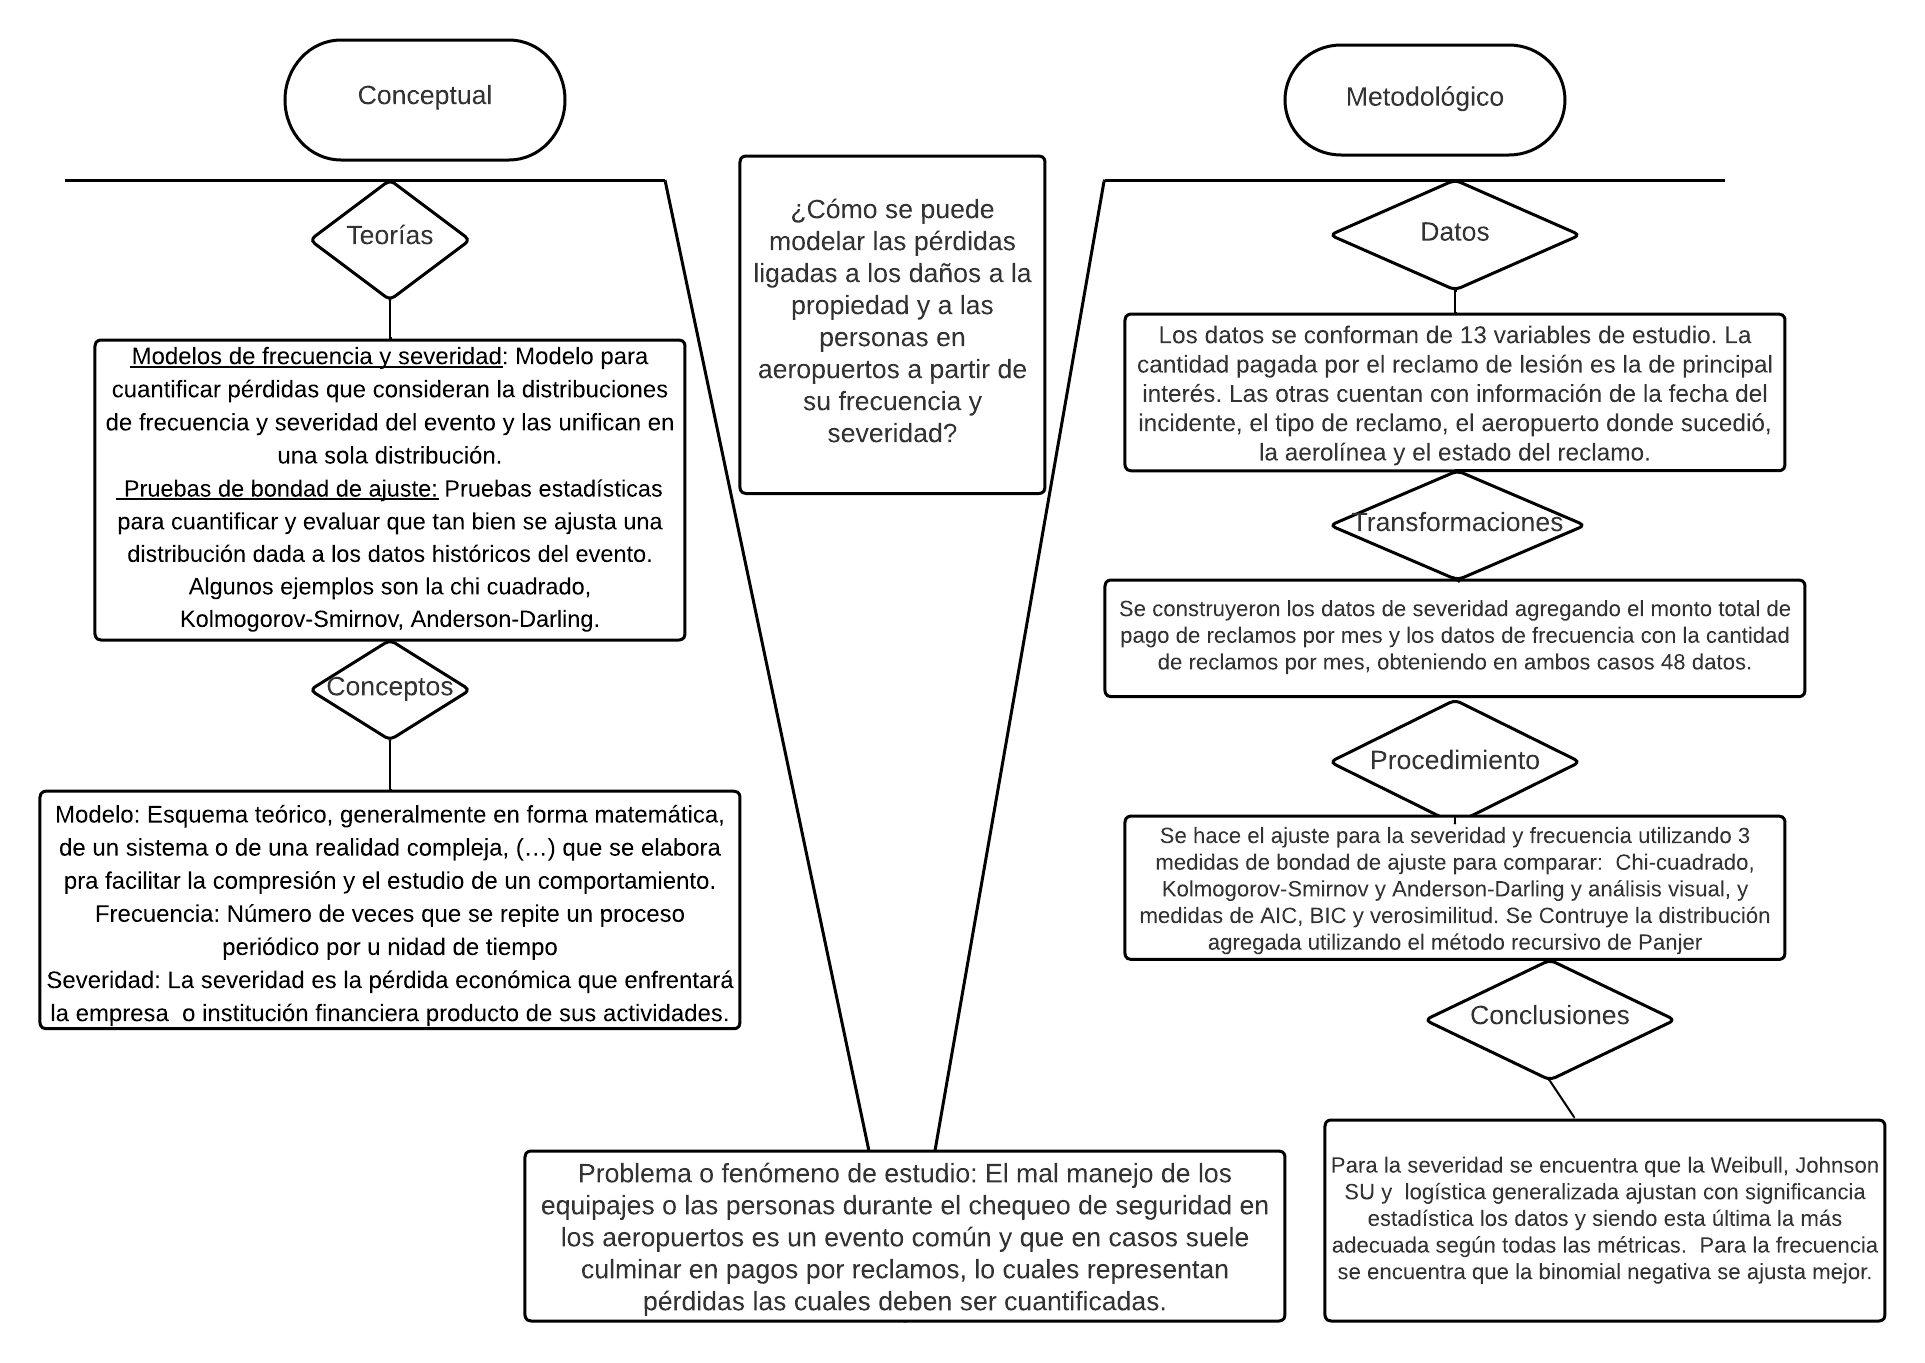
\includegraphics[width=6.25in,height=\textheight]{./Images/UVE Maik 3.png}

}

\end{figure}

\bookmarksetup{startatroot}

\hypertarget{bituxe1cora-4}{%
\chapter{Bitácora 4}\label{bituxe1cora-4}}

\hypertarget{parte-de-planificaciuxf3n-2}{%
\section{Parte de planificación}\label{parte-de-planificaciuxf3n-2}}

\hypertarget{variciones-en-el-ajuste-de-la-frecuencia}{%
\subsection{Variciones en el ajuste de la
frecuencia}\label{variciones-en-el-ajuste-de-la-frecuencia}}

En la bitácora anterior se comentó que se valoraba probar con
distribuciones compuestas para mejorar el ajuste de la frecuencia,
buscando con estas una mayor flexibilidad. En ese sentido se probó con
las composiciones Poisson-Gaussiana inversa, Poisson-Geométrica
(Distribución Polya-Aeppli) y Binomial negativa-Poisson (Delaporte).

En la Figura~\ref{fig-ajusteComp} se presenta la comparación de las
funciones de distribución ajustadas en comparación con la distribución
empírica. Se puede observar que el ajuste no es adecuado.

\begin{figure}[H]

\caption{\label{fig-ajusteComp}Ajustes de la frecuencia con
distribuciones compuestas}

{\centering 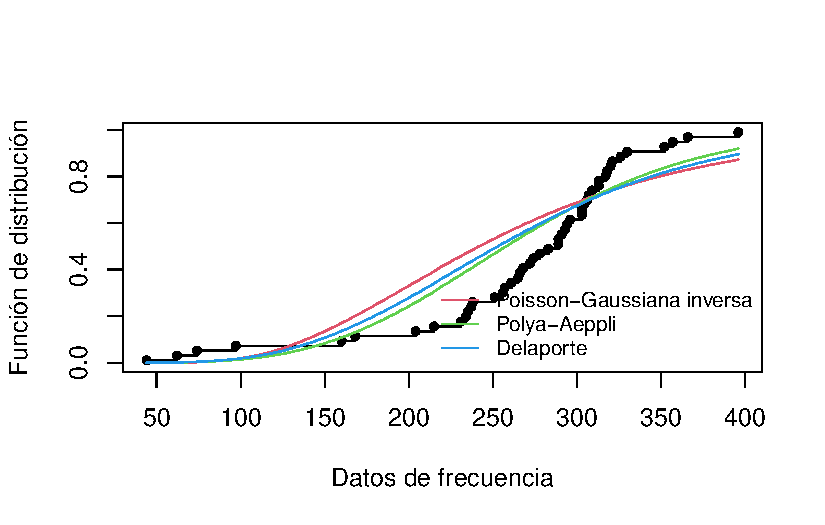
\includegraphics{./Bit4_files/figure-pdf/fig-ajusteComp-1.pdf}

}

\end{figure}

Además, se halló que versiones discretas de distribuciones continuas
podrían ser usadas para la modelización de la frecuencia. En este
análisis nos centramos en las variaciones disponibles en el paquete
\texttt{extraDistr} de \texttt{R}: la distribución Weibull discreta y la
Gamma discreta. En este contexto, la discretización corresponde a que es
la distribución de la parte entera de una variable aleatoria
absolutamente continua. La comparación de las distribuciones teóricas
ajustadas y la empírica se muestra en la figura
Figura~\ref{fig-ajusteVersionesDiscretas} y se nota que estos ajustes
son los mejores hasta el momento.

\begin{figure}[H]

\caption{\label{fig-ajusteVersionesDiscretas}Ajustes de la frecuencia
con distribuciones compuestas}

{\centering 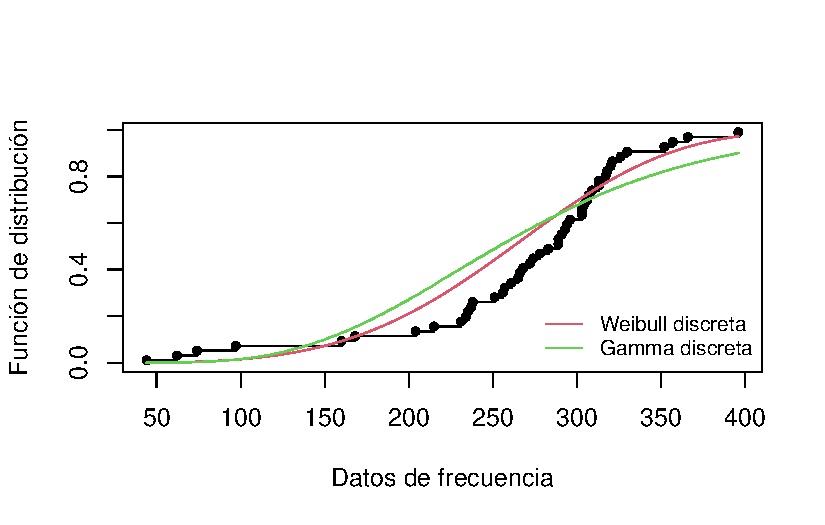
\includegraphics{./Bit4_files/figure-pdf/fig-ajusteVersionesDiscretas-1.pdf}

}

\end{figure}

Revisando el histograma en la Figura~\ref{fig-histograma_frecuencia}
surge la idea de probar con mezclas de distribuciones discretas, ya que
parece haber una porción hacia el inicio un poco desligada del resto.

\begin{figure}[H]

\caption{\label{fig-histograma_frecuencia}Histograma de frecuencia de
los reclamos por mes}

{\centering 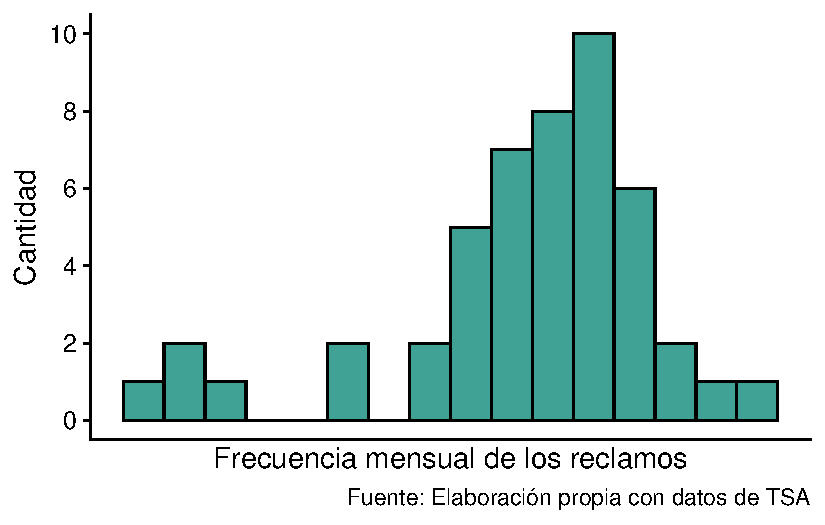
\includegraphics{./Bit4_files/figure-pdf/fig-histograma_frecuencia-1.pdf}

}

\end{figure}

Los ajustes con mezclas se limitaron a combinaciones de dos, tres,
cuatro y seis distribuciones de tipo Poisson. Debe señalarse un punto
muy importante respecto a estas mezclas: requieren estimar muchos
parámetros. Para explicar esta aseveración, téngase en cuenta que si
\(p(x;\lambda_{j})\) denota la función masa de probabilidad de una
distribución tipo Poisson con parámetro \(\lambda_{j}\), una mezcla de
\(d\) distribuciones tipo Poisson tiene función masa \[
p(x;\lambda_{1},\dots, \lambda_{d}, \alpha_{1},\dots, \alpha_{d})=\sum_{j=1}^{d}
\alpha_{j}\,p(x;\lambda_{j})
\] para algunos pesos \(\alpha_{j}\) que cumplen con ser positivos y
sumar la unidad. De este último hecho, se desprende que solamente es
necesario estimar \(d-1\) pesos, además de los \(d\) parámetros
\(\lambda_{j}\), sumando un total de \(2d-1\) parámetros a estimar. Es
decir, que con mezclas de dos, tres, cuatro y seis distribuciones tipo
Poisson, deben estimarse tres, cinco, siete y once parámetros
respectivamente. Como se mencionó en bitácoras anteriores, los datos de
frecuencia que se busca ajustar son un total de 48, de modo que estos
resultados deben tratarse con reserva, principalmente en los dos últimos
casos.

En las Figuras \ref{fig-ajusteMezclasPoisson23} y
\ref{fig-ajusteMezclasPoisson46} se presentan estos ajustes.
Visualmente, el ajuste en la Figura~\ref{fig-ajusteMezclasPoisson23} sin
duda mejora respecto a cualquier propuesta anterior y el de la
Figura~\ref{fig-ajusteMezclasPoisson46} es muy bueno. Sin embargo, sobre
todo este último ajuste debe manejarse con mucho cuidado ya que se
considera que ambos modelos exhiben sobreajuste.

\begin{figure}[H]

\caption{\label{fig-ajusteMezclasPoisson23}Ajustes de la frecuencia con
mezclas de dos y tres distribuciones tipo Poisson}

{\centering 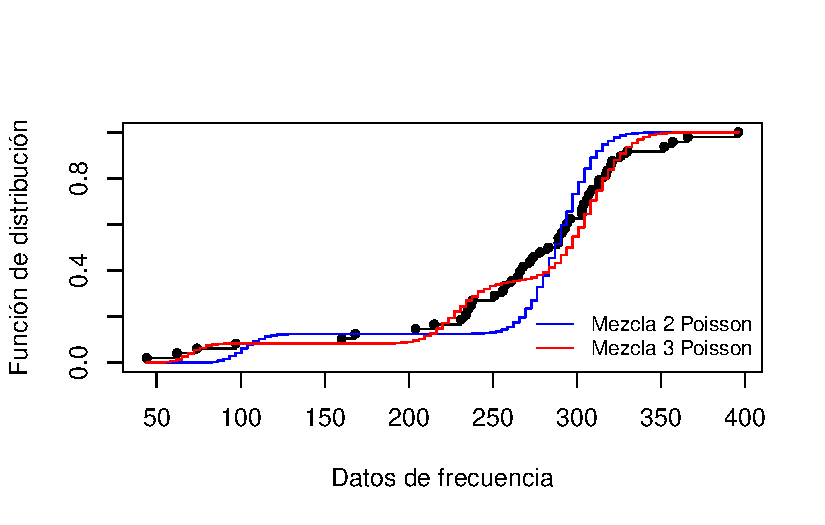
\includegraphics{./Bit4_files/figure-pdf/fig-ajusteMezclasPoisson23-1.pdf}

}

\end{figure}

\begin{figure}[H]

\caption{\label{fig-ajusteMezclasPoisson46}Ajustes de la frecuencia con
mezclas de cuatro y seis distribuciones tipo Poisson}

{\centering 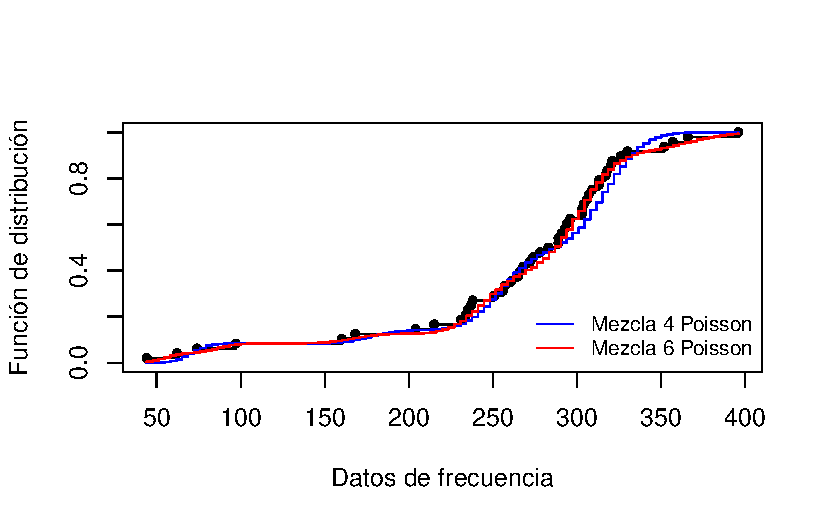
\includegraphics{./Bit4_files/figure-pdf/fig-ajusteMezclasPoisson46-1.pdf}

}

\end{figure}

\hypertarget{tbl-metricasNuevasFrecuencia}{}
\begin{table}
\caption{\label{tbl-metricasNuevasFrecuencia}Métricas de los modelos nuevos ajustados para la frecuencia }\tabularnewline

\centering
\begin{tabular}{l|l|l|l}
\hline
\textbf{Distribución} & \textbf{AIC} & \textbf{BIC} & \textbf{Valor $p$}\\
\hline
\cellcolor{gray!6}{Poisson-Gaussiana inversa} & \cellcolor{gray!6}{593.05} & \cellcolor{gray!6}{596.79} & \cellcolor{gray!6}{0}\\
\hline
Polya-Aeppli & 568.52 & 572.27 & 0.000042\\
\hline
\cellcolor{gray!6}{Delaporte} & \cellcolor{gray!6}{577.51} & \cellcolor{gray!6}{583.12} & \cellcolor{gray!6}{0}\\
\hline
Weibull discreta & 554.17 & 557.91 & 0.005499\\
\hline
\cellcolor{gray!6}{Gamma discreta} & \cellcolor{gray!6}{575.9} & \cellcolor{gray!6}{579.65} & \cellcolor{gray!6}{0.000002}\\
\hline
Mezcla 2 Poisson & 767.91 & 773.53 & 0\\
\hline
\cellcolor{gray!6}{Mezcla 3 Poisson} & \cellcolor{gray!6}{607.52} & \cellcolor{gray!6}{616.88} & \cellcolor{gray!6}{0.006487}\\
\hline
Mezcla 4 Poisson & 568.45 & 581.55 & \\
\hline
\cellcolor{gray!6}{Mezcla 6 Poisson} & \cellcolor{gray!6}{544.93} & \cellcolor{gray!6}{565.51} & \cellcolor{gray!6}{}\\
\hline
\end{tabular}
\end{table}

\hypertarget{ajuste-del-muxe1ximo}{%
\subsection{Ajuste del máximo}\label{ajuste-del-muxe1ximo}}

\begin{figure}[H]

{\centering 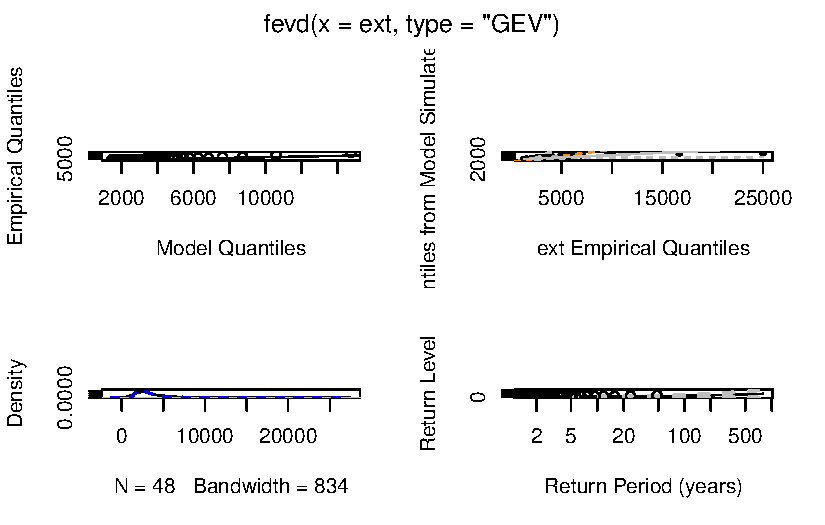
\includegraphics{./Bit4_files/figure-pdf/unnamed-chunk-11-1.pdf}

}

\end{figure}

\begin{figure}[H]

{\centering 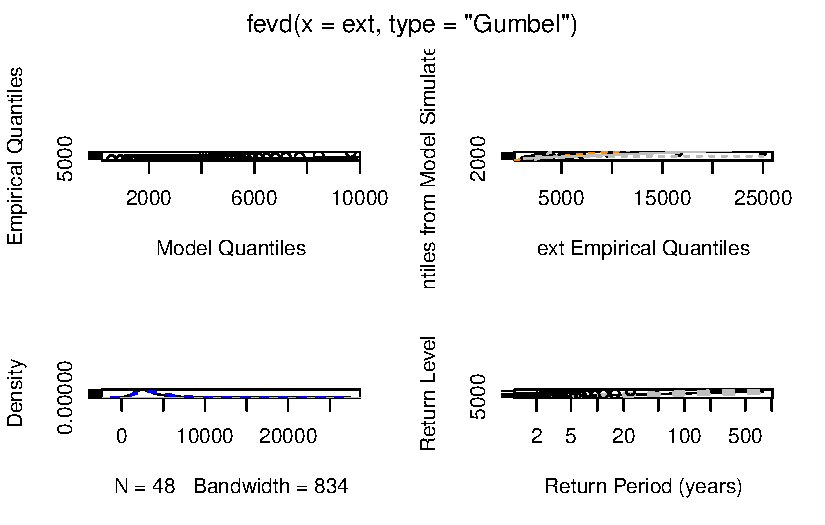
\includegraphics{./Bit4_files/figure-pdf/unnamed-chunk-12-1.pdf}

}

\end{figure}

\begin{figure}[H]

{\centering 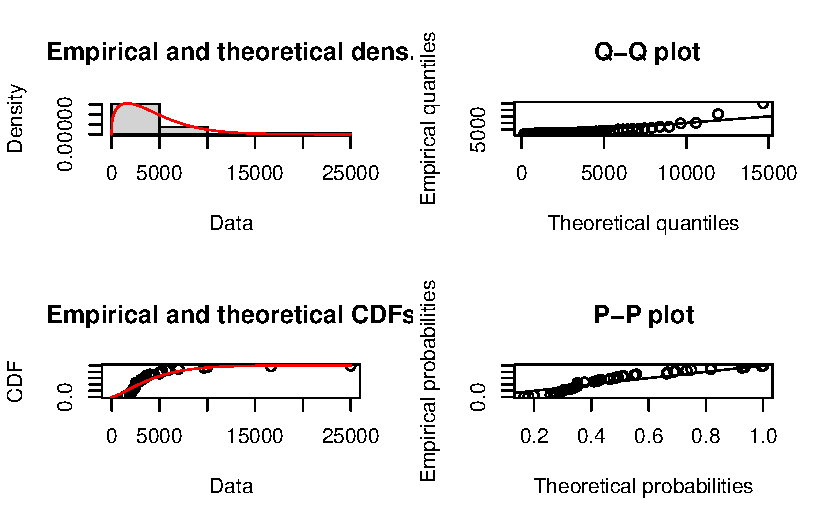
\includegraphics{./Bit4_files/figure-pdf/unnamed-chunk-13-1.pdf}

}

\end{figure}

AIC

\begin{verbatim}
[1] 860.7
\end{verbatim}

\begin{verbatim}
[1] 888
\end{verbatim}

\begin{verbatim}
[1] 894.4
\end{verbatim}

BIC

\begin{verbatim}
[1] 866.3
\end{verbatim}

\begin{verbatim}
[1] 891.7
\end{verbatim}

\begin{verbatim}
[1] 898.2
\end{verbatim}

\hypertarget{parte-de-escritura-2}{%
\section{Parte de escritura}\label{parte-de-escritura-2}}

\bookmarksetup{startatroot}

\hypertarget{referencias}{%
\chapter*{Referencias}\label{referencias}}
\addcontentsline{toc}{chapter}{Referencias}

\hypertarget{refs}{}
\begin{CSLReferences}{1}{0}
\leavevmode\vadjust pre{\hypertarget{ref-chakraborty2015generating}{}}%
Chakraborty, S. (2015). Generating discrete analogues of continuous
probability distributions-A survey of methods and constructions.
\emph{Journal of Statistical Distributions and Applications},
\emph{2}(1), 1-30.

\leavevmode\vadjust pre{\hypertarget{ref-chen2020aggregate}{}}%
Chen, S. (2020). \emph{Agrregate Loss Model with Poisson-Tweedie Loss
Frequency}.

\leavevmode\vadjust pre{\hypertarget{ref-soadefinitions}{}}%
Feldman, J., \& Brown, R. (2005). \emph{Risk and insurance}.

\leavevmode\vadjust pre{\hypertarget{ref-flores}{}}%
Flores, R. C. (2022). \emph{Modelling dependencies in airport passenger:
claim data using copulas} {[}Tesis doctoral{]}. Instituto Superior de
Economia e Gest{ã}o.

\leavevmode\vadjust pre{\hypertarget{ref-datos}{}}%
Homeland Security, D. of. (2015). \emph{TSA claims data}.
\url{https://www.dhs.gov/tsa-claims-data}

\leavevmode\vadjust pre{\hypertarget{ref-kelly2020data}{}}%
Kelly, M., \& Wang, Z. (2020). A data set for modeling claims
processes---tsa claims data. \emph{Risk Management and Insurance
Review}, \emph{23}(3), 269-276.

\leavevmode\vadjust pre{\hypertarget{ref-klugman2019loss}{}}%
Klugman, S., Panjer, H., \& Willmot, G. (2019). \emph{Loss Models From
Data ro Decisions, 5 th., vol. 6, no. 1. Hoboken}. New Jersey: John
Wiley \& Sons, Inc.

\leavevmode\vadjust pre{\hypertarget{ref-lyu2022discrete}{}}%
Lyu, J., \& Nadarajah, S. (2022). Discrete lognormal distributions with
application to insurance data. \emph{International Journal of System
Assurance Engineering and Management}, \emph{13}(3), 1268-1282.

\leavevmode\vadjust pre{\hypertarget{ref-cyprian}{}}%
Ondieki, C., Gathoni, S., \& Wairimu, J. (2018). \emph{Modeling the
Frequency and Severity of Auto Insurance Claims Using Statistical
Distributions}.

\leavevmode\vadjust pre{\hypertarget{ref-pitt2011estimation}{}}%
Pitt, D., Guillen, M., \& Bolancé, C. (2011). \emph{Estimation of
parametric and nonparametric models for univariate claim severity
distributions: an approach using R}.

\leavevmode\vadjust pre{\hypertarget{ref-vila2019theoretical}{}}%
Vila, R., Nakano, E. Y., \& Saulo, H. (2019). Theoretical results on the
discrete Weibull distribution of Nakagawa and Osaki. \emph{Statistics},
\emph{53}(2), 339-363.

\end{CSLReferences}



\end{document}
